% Options for packages loaded elsewhere
\PassOptionsToPackage{unicode}{hyperref}
\PassOptionsToPackage{hyphens}{url}
\PassOptionsToPackage{dvipsnames,svgnames,x11names}{xcolor}
%
\documentclass[
  letterpaper,
  DIV=11,
  numbers=noendperiod]{scrreprt}

\usepackage{amsmath,amssymb}
\usepackage{iftex}
\ifPDFTeX
  \usepackage[T1]{fontenc}
  \usepackage[utf8]{inputenc}
  \usepackage{textcomp} % provide euro and other symbols
\else % if luatex or xetex
  \usepackage{unicode-math}
  \defaultfontfeatures{Scale=MatchLowercase}
  \defaultfontfeatures[\rmfamily]{Ligatures=TeX,Scale=1}
\fi
\usepackage{lmodern}
\ifPDFTeX\else  
    % xetex/luatex font selection
\fi
% Use upquote if available, for straight quotes in verbatim environments
\IfFileExists{upquote.sty}{\usepackage{upquote}}{}
\IfFileExists{microtype.sty}{% use microtype if available
  \usepackage[]{microtype}
  \UseMicrotypeSet[protrusion]{basicmath} % disable protrusion for tt fonts
}{}
\makeatletter
\@ifundefined{KOMAClassName}{% if non-KOMA class
  \IfFileExists{parskip.sty}{%
    \usepackage{parskip}
  }{% else
    \setlength{\parindent}{0pt}
    \setlength{\parskip}{6pt plus 2pt minus 1pt}}
}{% if KOMA class
  \KOMAoptions{parskip=half}}
\makeatother
\usepackage{xcolor}
\setlength{\emergencystretch}{3em} % prevent overfull lines
\setcounter{secnumdepth}{5}
% Make \paragraph and \subparagraph free-standing
\ifx\paragraph\undefined\else
  \let\oldparagraph\paragraph
  \renewcommand{\paragraph}[1]{\oldparagraph{#1}\mbox{}}
\fi
\ifx\subparagraph\undefined\else
  \let\oldsubparagraph\subparagraph
  \renewcommand{\subparagraph}[1]{\oldsubparagraph{#1}\mbox{}}
\fi


\providecommand{\tightlist}{%
  \setlength{\itemsep}{0pt}\setlength{\parskip}{0pt}}\usepackage{longtable,booktabs,array}
\usepackage{calc} % for calculating minipage widths
% Correct order of tables after \paragraph or \subparagraph
\usepackage{etoolbox}
\makeatletter
\patchcmd\longtable{\par}{\if@noskipsec\mbox{}\fi\par}{}{}
\makeatother
% Allow footnotes in longtable head/foot
\IfFileExists{footnotehyper.sty}{\usepackage{footnotehyper}}{\usepackage{footnote}}
\makesavenoteenv{longtable}
\usepackage{graphicx}
\makeatletter
\def\maxwidth{\ifdim\Gin@nat@width>\linewidth\linewidth\else\Gin@nat@width\fi}
\def\maxheight{\ifdim\Gin@nat@height>\textheight\textheight\else\Gin@nat@height\fi}
\makeatother
% Scale images if necessary, so that they will not overflow the page
% margins by default, and it is still possible to overwrite the defaults
% using explicit options in \includegraphics[width, height, ...]{}
\setkeys{Gin}{width=\maxwidth,height=\maxheight,keepaspectratio}
% Set default figure placement to htbp
\makeatletter
\def\fps@figure{htbp}
\makeatother
\newlength{\cslhangindent}
\setlength{\cslhangindent}{1.5em}
\newlength{\csllabelwidth}
\setlength{\csllabelwidth}{3em}
\newlength{\cslentryspacingunit} % times entry-spacing
\setlength{\cslentryspacingunit}{\parskip}
\newenvironment{CSLReferences}[2] % #1 hanging-ident, #2 entry spacing
 {% don't indent paragraphs
  \setlength{\parindent}{0pt}
  % turn on hanging indent if param 1 is 1
  \ifodd #1
  \let\oldpar\par
  \def\par{\hangindent=\cslhangindent\oldpar}
  \fi
  % set entry spacing
  \setlength{\parskip}{#2\cslentryspacingunit}
 }%
 {}
\usepackage{calc}
\newcommand{\CSLBlock}[1]{#1\hfill\break}
\newcommand{\CSLLeftMargin}[1]{\parbox[t]{\csllabelwidth}{#1}}
\newcommand{\CSLRightInline}[1]{\parbox[t]{\linewidth - \csllabelwidth}{#1}\break}
\newcommand{\CSLIndent}[1]{\hspace{\cslhangindent}#1}

\KOMAoption{captions}{tableheading}
\makeatletter
\makeatother
\makeatletter
\@ifpackageloaded{bookmark}{}{\usepackage{bookmark}}
\makeatother
\makeatletter
\@ifpackageloaded{caption}{}{\usepackage{caption}}
\AtBeginDocument{%
\ifdefined\contentsname
  \renewcommand*\contentsname{Table of contents}
\else
  \newcommand\contentsname{Table of contents}
\fi
\ifdefined\listfigurename
  \renewcommand*\listfigurename{List of Figures}
\else
  \newcommand\listfigurename{List of Figures}
\fi
\ifdefined\listtablename
  \renewcommand*\listtablename{List of Tables}
\else
  \newcommand\listtablename{List of Tables}
\fi
\ifdefined\figurename
  \renewcommand*\figurename{Figure}
\else
  \newcommand\figurename{Figure}
\fi
\ifdefined\tablename
  \renewcommand*\tablename{Table}
\else
  \newcommand\tablename{Table}
\fi
}
\@ifpackageloaded{float}{}{\usepackage{float}}
\floatstyle{ruled}
\@ifundefined{c@chapter}{\newfloat{codelisting}{h}{lop}}{\newfloat{codelisting}{h}{lop}[chapter]}
\floatname{codelisting}{Listing}
\newcommand*\listoflistings{\listof{codelisting}{List of Listings}}
\makeatother
\makeatletter
\@ifpackageloaded{caption}{}{\usepackage{caption}}
\@ifpackageloaded{subcaption}{}{\usepackage{subcaption}}
\makeatother
\makeatletter
\@ifpackageloaded{tcolorbox}{}{\usepackage[skins,breakable]{tcolorbox}}
\makeatother
\makeatletter
\@ifundefined{shadecolor}{\definecolor{shadecolor}{rgb}{.97, .97, .97}}
\makeatother
\makeatletter
\makeatother
\makeatletter
\makeatother
\ifLuaTeX
  \usepackage{selnolig}  % disable illegal ligatures
\fi
\IfFileExists{bookmark.sty}{\usepackage{bookmark}}{\usepackage{hyperref}}
\IfFileExists{xurl.sty}{\usepackage{xurl}}{} % add URL line breaks if available
\urlstyle{same} % disable monospaced font for URLs
\hypersetup{
  pdftitle={Türkiye Kuşları},
  pdfauthor={Kerem Ali Boyla},
  colorlinks=true,
  linkcolor={blue},
  filecolor={Maroon},
  citecolor={Blue},
  urlcolor={Blue},
  pdfcreator={LaTeX via pandoc}}

\title{Türkiye Kuşları}
\author{Kerem Ali Boyla}
\date{2024-01-18}

\begin{document}
\maketitle
\ifdefined\Shaded\renewenvironment{Shaded}{\begin{tcolorbox}[boxrule=0pt, frame hidden, enhanced, sharp corners, breakable, borderline west={3pt}{0pt}{shadecolor}, interior hidden]}{\end{tcolorbox}}\fi

\renewcommand*\contentsname{Table of contents}
{
\hypersetup{linkcolor=}
\setcounter{tocdepth}{2}
\tableofcontents
}
\bookmarksetup{startatroot}

\hypertarget{kitap-hakkux131nda}{%
\chapter*{Kitap Hakkında}\label{kitap-hakkux131nda}}
\addcontentsline{toc}{chapter}{Kitap Hakkında}

\markboth{Kitap Hakkında}{Kitap Hakkında}

Türkiye farklı kıtalara yakınlığı, zengin coğrafyası ve ana göç yolları
üzerindeki konumu nedeniyle zengin bir kuş faunası barındırır. Bu kitap
Türkiye'de görülen kuşlar hakkındaki en güncel, kapsamlı ve güvenilir
referans kaynağı olmayı hedefler. Ülke listesindeki bütün türlerin
mevcut durumu, coğrafi yayılışı, göç hareketleri, üreme biyolojisi ve
taksonomik durumu verilmiştir. Bu kitapta en güncel gözlemler,
ornitolojik yayınlar ve raporlardan faydalanılmıştır. Bu kitabın hedef
kitlesi kuş gözlemcileri, doğa korumacıları ve bilim insanlarıdır.

Kuşları doğada gözlemek ve tanımlamak bu kitabın kapsamı dışındadır.
Saha rehberi olarak aşağıdaki kaynaklardan faydalanılabilir: Trakus --
Türkiye'nin Kuşları (2021), Türkiye ve Ortadoğu'nun Kuşları (2009), Kuş
Gözlemcisinin Cep Kitabı (2005) ve Türkiye ve Avrupa'nın Kuşları (2001).

\hypertarget{kitabux131n-iuxe7eriux11fi}{%
\section*{Kitabın İçeriği}\label{kitabux131n-iuxe7eriux11fi}}
\addcontentsline{toc}{section}{Kitabın İçeriği}

\markright{Kitabın İçeriği}

Kitabın içeriği hazırlandığı sürece yayına verilecektir. Kitabın tamamı
31 Aralık 2024 tarihine kadar tamamlanacaktır. Kitabın bölümleri:

\begin{itemize}
\tightlist
\item
  Ördekgiller (güncelleniyor)
\item
  Tavukgiller (güncelleniyor)
\item
  Balıkçıllar ve diğerleri (güncelleniyor)
\item
  Yırtıcılar
\item
  Bataklık ve Kır Kuşları
\item
  Cılıbıtgiller
\item
  Çullukgiller
\item
  Martılar
\item
  Kara Kuşları
\item
  Ötücü Öncesi Grup: Papağanlar, Ağaçkakanlar ve Doğanlar
\item
  Ötücüler - Kargamsılar
\item
  Ötücüler - Ötleğenimsiler: Toygarlar
\item
  Ötücüler - Ötleğenimsiler: Çıvgınler
\item
  Ötücüler - Ötleğenimsiler: Ötleğenler
\item
  Ötücüler - Tırmaşığımsılar
\item
  Ötücüler - Sinekkapanımsılar
\item
  Ötücüler - Serçemsiler: İncirkuşugiller, Dağbülbülleri ve Serçeler
\item
  Ötücüler - Serçemsiler: İspinozlar ve Çinteler
\end{itemize}

\hypertarget{neden-dijital-bir-kitap}{%
\section*{Neden Dijital Bir Kitap?}\label{neden-dijital-bir-kitap}}
\addcontentsline{toc}{section}{Neden Dijital Bir Kitap?}

\markright{Neden Dijital Bir Kitap?}

Bu kitap, 2008 yılında yayımlanan ``The Birds of Turkey'' kitabının
Türkçe'ye çevrilmesi düşüncesinden doğmuştur. İlk çeviri taslakları
oluşunca, dünyanın en zengin ornitoloji külliyatına sahip olan İngilizce
dilindeki metnin anlaşılır bir şekilde Türkçeye çevirmenin zor olacağı
tespit edildi. Dahası, metnin mevcut halinin okuyucu tarafından kolayca
anlaşılamayacağı ve hatta aşırı akademik bulunabileceği fark edildi.

Bunun üzerine metnin tamamen gözden geçirilmesi zorunlu hale geldi.
Türkiye sınırları dışındaki bilimsel içerik kapsam dışı bırakıldı. ``The
Birds of Turkey'' kitabının yayımlanmasından bu yana geçen 15 yıl
boyunca, Türkiye'deki kuş faunasındaki gelişmeler ve kuş gözlemciliğinin
yaygınlaşması sayesinde artan bilgilerle metin ve haritalar güncellendi.
Kitabın okunabilirliğini artırmak için mevcut durum paragrafı ve
vinyetler gibi okuyucu dostu unsurlar eklendi, haritalar renklendirildi
ve iyileştirildi, kaynakça için numaralandırılmış bir sistem getirildi.
Başlangıçta bir çeviri projesi olarak başlayan bu çalışma, özgün içeriğe
sahip yeni bir kitaba dönüştü.

Peki, neden dijital bir kitap? Bu yeni kitabın basılı bir yayın olarak
değil, açık kaynak dijital bir kitap formatında yayınlanmasının
nedenlerini şu şekilde sıralayabilirim:

\begin{itemize}
\item
  Kuşlar gibi dinamik bir konu hakkında yazılan her kitap, basıldığı gün
  güncelliğini kaybeder. Dijital bir kitabın sık sık güncellenmesi ise
  mümkün ve kolaydır.
\item
  Bu teknik kitabın içeriği, bir yazar ve bir editör arasında gidip
  gelen metinlerle sınırlı kalmamalıdır. Dijital formatta içerik
  hakkında bilgi sahibi olan geniş bir kitlenin katkısı alınabilir.
\item
  Açık kaynak olan dijital müsvedde (manuskript) herkesin erişimine
  ücretsiz olarak açıktır ve bu sayede kuş bilimi (ornitoloji), kuşların
  tanınması ve doğa koruma ile ilgilenen herkes faydalanabilir. Üstelik
  uzmanlar ve akademisyenler GitHUb üzerinden metni doğrudan
  düzenleyebilirler.
\item
  Kitaptaki kuş türleri veya kuşların yayılış haritaları, eBird gibi
  açık kaynak veri tabanlarından gelen verilerle hızlı, hatta anlık
  olarak güncellenebilir.
\item
  Bir kitaptaki sayfa sayısını ekonomik nedenler ve kullanışı
  zorlaştırmamak için yaklaşık 500 sayfa ile sınırlamak gerekebilir.
  Dijital bir kitapta teknik bir sınırlama yoktur.
\item
  Elbette bu çalışmanın kalıcı olması için bir kitap olarak basılması
  her yazarın hayalidir. Dijital format sayesinde yüzlerce hatta
  binlerce okuyucu tarafından revize edilmiş ve içeriği iyileştirilmiş
  bir metnin yayına hazırlanması daha kolaydır.
\item
  İçeriğini tamamının hazır olmadığı durumda, dijital kitabı fasiküller
  halinde yayımlamak mümkündür.
\end{itemize}

Kitabın internet formatındaki versiyonu
\href{https://quarto.org/}{Quarto publishing system} ile hazıranmıştır.

\hypertarget{duxfczeltme-uxf6nerileri}{%
\section*{Düzeltme Önerileri}\label{duxfczeltme-uxf6nerileri}}
\addcontentsline{toc}{section}{Düzeltme Önerileri}

\markright{Düzeltme Önerileri}

Metinde bulduğunuz yazım hatalarını, eksik bilgileri, kaynakları ve
diğer düzeltme önerilinizi bana gönderebilirsiniz: kerem.boyla@gmail.com

Ayrıca uzman ve akademisyenler GitHub üzerinden metinlere erişebilirler
ve düzeltmelerini gönderebilirler.

\hypertarget{telif-hakkux131}{%
\section*{Telif Hakkı}\label{telif-hakkux131}}
\addcontentsline{toc}{section}{Telif Hakkı}

\markright{Telif Hakkı}

Bu kitap \href{https://creativecommons.org/licenses/by/4.0/}{Creative
Commons Attribution 4.0 International License} ile lisanslanmıştır.
Kitabının tüm hakları yazarlarına aittir. Bu, kitabın kopyalanması,
dağıtılması, sergilenmesi, ve eserden türetilmiş çalışmaların
oluşturulması dahil olmak üzere birçok faaliyeti serbest bırakır, ancak
eser üzerindeki orijinal yazarları belirtmeniz şarttır.

Boyla, K.A. (2024) Türkiye Kuşları.
\url{https://keremaliboyla.github.io/turkiye-kuslari/}

\bookmarksetup{startatroot}

\hypertarget{uxf6rdekgiller}{%
\chapter{Ördekgiller}\label{uxf6rdekgiller}}

\hypertarget{boz-kaz}{%
\section{Boz Kaz}\label{boz-kaz}}

\emph{Anser anser}, Greylag Goose

\textbf{\emph{Lokal olarak az sayıda ürer. Kışın göç alır ve daha geniş
bir yayılış gösterir.}}

Üreme döneminde az sayıda Göller Bölgesi, İç Anadolu ve Doğu Anadolu'da
bataklık sulakalanlarda bulunur. Eskiden Sultansazlığı gibi birkaç
alanda yüksek sayıda üremiştir. Türkiye Kuş
Raporları\textsuperscript{1--11} üreyen popülasyonun son 50 yılda çok
ciddi bir düşüş yaşadığını gösterir. Eskiden ürediği sulakalanların çoğu
kurutulmuştur. Örneğin, Ereğli Sazlığı'nda Nisan 1970'te 120 yuva ve 300
birey varken, Temmuz 1996'da 160 birey sayılmış, bugün ise hiçbir üreyen
çift kalmamıştır.

Üreme sonrasında tüy dökümü sırasında kalabalık sürüler bazı
sulakalanlarda toplanır; Temmuz 1984'te Kulu Gölü'nde 800 birey,
bilinmeyen bir tarihte Sultansazlığı'nda 12.000 birey ve Eylül 2004'de
Kuyucuk Gölü'nde 10.000 birey kaydedilmiştir.

Geçiş sırasında tüm bölgelerde da görülen, ekimden itibaren mart sonuna
kadar kalan bir kış göçmenidir. Kışlayan sürüler genellikle kıyısal
bölgelerde yoğunlaşır. Son yıllarda görülen sürüler 300 bireyden azdır.
KOSKS verilerine göre eskiden daha bol bulunurdu, genellikle ortalama
5000 birey, en yüksek 1967'de 11.200 birey tespit edilmiştir. Alanlarda
yapılan sayımlarda Kızılırmak Deltası'nda 5000 birey, Meriç Deltası'nda
4500 birey ve Hotamış Sazlığı'nda 1500 birey tespit edilmiştir.

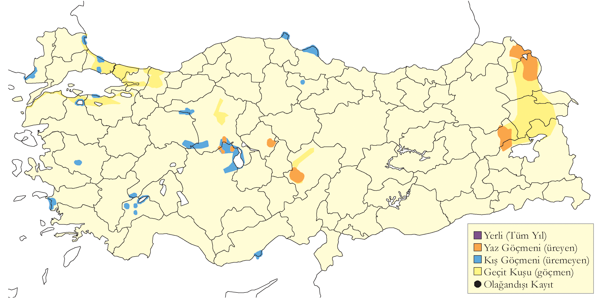
\includegraphics{images/harita_Page_002.png}

\hypertarget{uxfcreme}{%
\subsection{\texorpdfstring{\textbf{Üreme}}{Üreme}}\label{uxfcreme}}

\textbf{Yuvalama alanı:} Göllerdeki adalarda genellikle küçük gruplar
halinde ürer.\\
\textbf{Yuvası}: Kulu Gölü'nde gözlenen yuvası kuru toprağa kazılmış sığ
bir çukurdur ve çevredeki bitki örtüsü ve küçük tüylerle astarlanmıştır.
Ereğli Sazlığı'ndaki yuvası saz ve diğer sucul bitkilerden oluşan ve su
seviyesinin üstünde kalan bir yapının üzerine kurmuştur.\\
\textbf{Yumurta sayısı:} Türkiye'de yumurta sayısına ilişkin güvenilir
gözlem yoktur. Yuvadan ayrılmış beş kaz yavrusu, görülen en kalabalık
gruptur. Diğer ülkelerde genellikle 4-6 yumurta koyar.\\
\textbf{Üreme dönemi:} Mart sonunda yumurta koyar. En erken yavrular 23
Nisan 1988'de Kulu Gölü'nde, 27 Nisan 1988'de Sultansazlığı'nda, 30
Nisan 1968'de Mogan Gölü'nde ve 30 Nisan 1973'de Ereğli Sazlıkları'nda
gözlenmiştir. 20 Nisan 1996'da Marmara'da, 14 Mayıs 1969'ta
Karadeniz'de, 16 Mayıs 1970'da ve 24 Haziran 1983'te Doğu Anadolu'da
kaydedilen yavrular gecikmiş üremeyi gösterir.

\textbf{Alttürler ve Sınıflandırma}

Ülkemizde \emph{rubrirostris} alttürü bulunur. Bu alttür turuncu
gagasıyla Batı ve Orta Avrupa'da bulunan pembe gagalı \emph{anser}
alttüründen ayrılır.

\hypertarget{sakarca}{%
\section{Sakarca}\label{sakarca}}

\emph{Anser albifrons}, Greater White-fronted Goose

\textbf{\emph{Lokal olarak bulunan ve zaman zaman kalabalık sürüler
oluşturan bir kış konuğudur.}}

Ekim sonu ile nisan başı arasında lokal olarak görülen bir kış
konuğudur. Genellikle ocak ve şubat ayında daha yaygın ve yüksek sayıda
olur. Soğuk geçen kışlar Türkiye'de kışlayan nüfusu artar. En kalabalık
sürüler Meriç Nehri boyunda, Tuz Gölü çevresinde ve Konya Ovasında
yoğunlaşır. Büyük Menderes Deltası ve Doğu Akdeniz sulakalanlarında
önemli sayılarda toplanabilir. Son zamanlarda Güneydoğu Anadolu'daki
baraj göllerinde küçük sürüler halinde görülmeye başlamıştır. Nadiren
yazın sulakalanlarda az sayıda kalabilir.

Kış ortası su kuşu sayımlarında (KOSKS) ülke genelinde en yüksek sayıda
1968-69 kışında 98.600 birey sayılmıştır. 1987'de toplam 84.000 birey
kaydedilmiştir. Daha sonra kışlayan sayılar ciddi bir düşüş yaşamıştır.
1990'lı yıllarda genellikle 20.000-30.000, 1993'de
11.822\textsuperscript{12}, 1999'da 3956\textsuperscript{13} ve 2005'te
3891 birey\textsuperscript{14} tespit edilmiştir. Kışın soğuk geçtiği 11
Şubat 2006'de Büyükçekmece'de sayılan 15.000 birey son yıllardaki en
yükse sayımdır. Dolayısıyla, Türkiy'de kışlayan nüfusun 1970'lerde
100.000'ler seviyesinden 2010'larda 5000 seviyesine indiği tespit
edilmiştir.

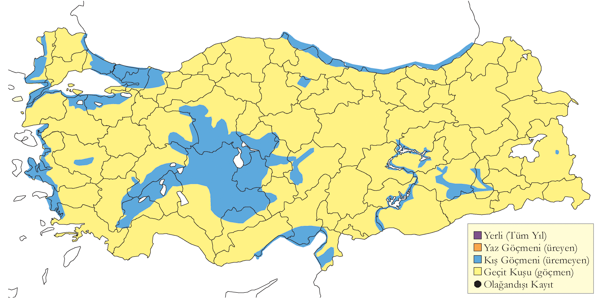
\includegraphics{images/harita_Page_003.png}

\hypertarget{uxfcreme-1}{%
\subsection{\texorpdfstring{\textbf{Üreme}}{Üreme}}\label{uxfcreme-1}}

Türkiye'de yuvalamaz. Avrasya ve Kuzey Amerika'nın tundra bölgelerinde
yuvalar.

\textbf{Alttürler ve Sınıflandırma}

Türkiye'de nominat alttürü bulunur.

\hypertarget{kuxfcuxe7uxfck-sakarca}{%
\section{Küçük Sakarca}\label{kuxfcuxe7uxfck-sakarca}}

\emph{Anser erythropus}, Lesser White-fronted Goose

\textbf{\emph{Az sayıda gelen düzenli kış konuğudur.}}

Her yıl çok az sayıda kaydedilen bir kış konuğudur. Hiçbir alanda
düzenli olarak bulunmadığı düşünülür. Sayıları genellikle 10'dan azdır.
Çoğunlukla diğer kaz türleri ile karışık olarak bulunur. Bugüne kadar,
Türkiye'ye gelen bireylerin İskandinavya'da üreyen ve Balkan ülkelerinde
kışlayan göçyolu (flyway) nüfusuna ait olduğu düşünüldü. Yunanistan'da
bir alanda kışlayan ve koruma çalışmaları nedeniyle sayıları artan
sürünün kış ortasında oradan kaybolması, Marmara ve Ege bölgelerinde bir
kışlama alanının ihtimalini doğurdu. Ancak yapılan aramalara rağmen
burada düzenli ziyaret edilen bir kışlama alanı bulunamadı.

Ülkenin diğer ucunda, 20 Kasım 2004'te Haçlı Gölünde uydudan izlenen bir
birey sinyal verince, doğuda bir kışlama alanın ihtimali
doğdu\textsuperscript{15}. Nitekim Van Gölü ve Erçek Gölü kıyılarında
sayıları 340'ı bulan kalabalık sürüler düzenli olarak tespit edildi.
Bugün ülkede kışlayan ana nüfusun Doğu Anadolu'da bulunduğu
söylenebilir\textsuperscript{16}.

2000 öncesindeki kayıtlara bakıldığında; 29 Aralık 1997'de Göksü
Deltası'nda bir birey\textsuperscript{6}, 23 Ocak 1993'te Göksu
Deltası'nda bir birey\textsuperscript{12}, 6 Nisan 1990'da Seyfe
Gölü'nde 12 birey\textsuperscript{9}, 24 Aralık 1986'da Bafa Gölü'nde
bir erişkin iki genç\textsuperscript{17} ve 16 Şubat 1967'da Kocabaş
Çayının ağzında (Çanakkale) iki birey\textsuperscript{1} kaydedilmiştir.
1945 ile 1965 ve ekim ile ocak arasında büyük çoğunluğu Büyükçekmece ve
Küçükçekmece göllerinden gelen 12 kaydı vardır. Ancak bu kayıtlar tür
tanımını destekleyecek belgeden yoksundur\textsuperscript{18}.

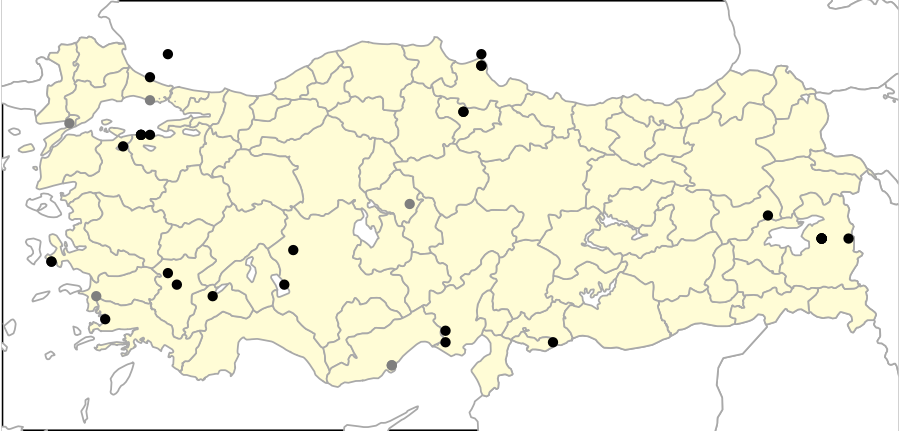
\includegraphics[width=6.25in,height=\textheight]{images/harita_Anser_erythropus.png}

\hypertarget{uxfcreme-2}{%
\subsection{\texorpdfstring{\textbf{Üreme}}{Üreme}}\label{uxfcreme-2}}

Türkiye'de yuvalamaz. Kuzey İskandinavya'dan Doğu Sibirya'ya uzanan
tundra kuşağında ürer.

\textbf{Alttürler ve Sınıflandırma}

Monotipik bir türdür.

\hypertarget{tundra-kazux131}{%
\section{Tundra Kazı}\label{tundra-kazux131}}

\emph{Anser serrirostris}, Tundra Bean Goose

\textbf{\emph{Nadiren gelen kış konuğudur.}}

2000 yılından sonra üç kere kaydedilmiştir. Birer birey 26 Şubat 2013'te
Yedikır Barajı'nda, 4-21 Şubat 2015'te Kızılırmak Deltası'nda ve Manyas
Gölü'nde 2 birey görülmüştür. Tür kış aylarında sakarca sürüleri
arasında bulunabilir.

Tundra Kazı, önceleri Tayga Kazı ile beraber tek bir tür altında Tarla
Kazı olarak sınıflandırılırdı. Dolayısıyla, taksonomik revizyonun
yapıldığı tarihin öncesindeki kayıtlarda Tarla Kazı olarak
tanımlanmıştır. 2000'den sonra çekilen fotoğraflarda özellikle gaga
renklenmesi incelenmiş, bu kuşların hepsi Tundra Kazı olarak
tanımlanmıştır. Fotoğrafı veya betimlemesi olmayan eski kayıtların hangi
türe ait olduğu belirsiz kalacaktır.

Tarla Kazı olarak tanımlanmış kuşlar Ege, Akdeniz ve İç Anadolu'daki
sulakalanlarda ara sıra yüksek sayılarda kaydedilmiştir. 1870'ler ve
1880'lerde Mersin'de toplanan bireyler\textsuperscript{19} ilk
kayıtlarıdır. 1966-2000 arasında çoğunlukla ocak ile mart arasında 15
kez kaydedilmiştir. 2 Mart 1965'te Ereğli ve Karapınar arasında 90
birey\textsuperscript{18}, 15-16 Ekim 1969'da Karamık Sazlıklarında 13
birey\textsuperscript{2}, 30 Nisan 1988'de Seyfe Gölü'nde, 30 Ocak
1992'de Marmara Gölü'nde 61 birey, 9 Ocak 1993'te Büyükçekmece Gölü'nde
64 birey\textsuperscript{12} ve 24 Ocak 1993'te Göksu Deltası'nda bir
birey\textsuperscript{12} kaydedilmiştir. Türkiye'deki kışlayan Sakarca
sayılarındaki sert düşüş muhtemelen Tarla Kazı olarak tanımlanmış kuşlar
için de geçerlidir.

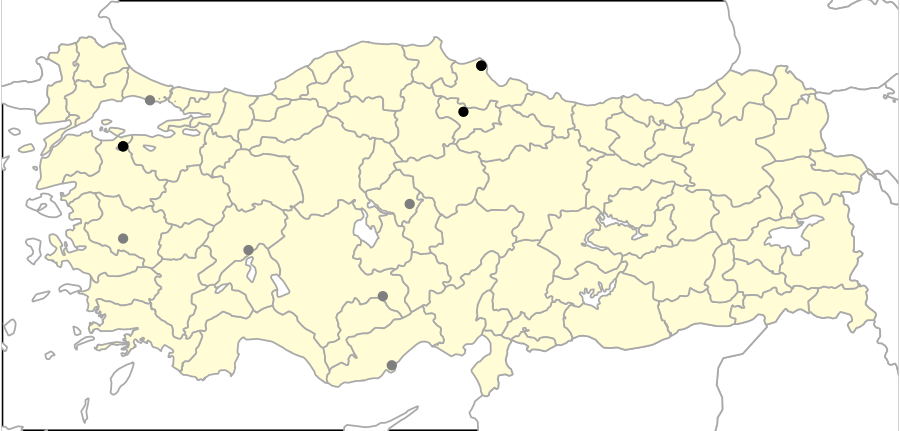
\includegraphics[width=6.25in,height=\textheight]{images/harita_Anser_serrirostris.png}

\hypertarget{uxfcreme-3}{%
\subsection{\texorpdfstring{\textbf{Üreme}}{Üreme}}\label{uxfcreme-3}}

Türkiye'de yuvalamaz. Üreme alanı Kuzey İskandinavya'dan Doğu Sibirya'ya
uzanan tundra kuşağındadır.

\textbf{Alttürler ve Sınıflandırma}

Tayga Kazı yeni bir türdür ve yakın zamana kadar Tarla Kazı olaran
bilinen bir türden ayrılmıştır. 5 alttürden oluşan Tarla Kazı
(\emph{Anser fabalis}) ikiye ayrılınca \emph{fabalis}, \emph{johanseni}
ve \emph{middendorffii} alttürleri Tayga Kazı (\emph{Anser fabalis}),
\emph{serrirostris} ve \emph{rossicus} alttürleri Tundra Kazı
(\emph{Anser serrirostris}) altında sınıflandırılmıştır.

\hypertarget{yosun-kazux131}{%
\section{Yosun Kazı}\label{yosun-kazux131}}

\emph{Branta bernicla}, Brant Goose

\textbf{\emph{Rastlantısal konuktur.}}

Batı Avrupa'da Atlantik kıyılarında kışlayan bir türdür. Türkiye ve
yakın coğrafyasında rastlantısal konuktur. 6 Nisan 1981'de Küçük
Menderes Deltası'nda iki birey\textsuperscript{5}, 3-4 Eylül 1973'te
Ardeşen açıklarında koyu karınlı \emph{bernicla} alttürüne ait iki birey
kaydedilmiştir\textsuperscript{3}. 1969 yılında Acıgöl'den gelen bir
iddia kabul edilmemiştir\textsuperscript{20}. 7 Şubat 1945'de
Büyükçekmece'de bir bireyi Prenses Zeyneb Halim vurmuştur, maalesef bu
kuşun gövdesi korunamamıştır\textsuperscript{18}. Kışın soğuk geçtiği
Ocak 1889'da düzenli olarak İstanbul Maltepe'de ve Şubat 1891'de büyük
sürüler halinde İstanbul Kadıköy'de görülmüştür\textsuperscript{21}.

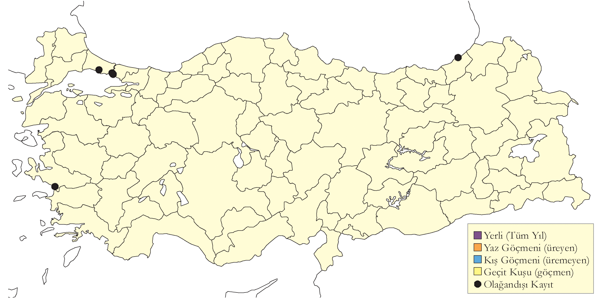
\includegraphics{images/harita_Page_005.png}

\hypertarget{uxfcreme-4}{%
\subsection{\texorpdfstring{\textbf{Üreme}}{Üreme}}\label{uxfcreme-4}}

Türkiye'de yuvalamaz. Orta ve Kuzey Sibirya'da Kuzey Kutup Denizi kıyı
şeridinde yuvalar.

\textbf{Alttürler ve Sınıflandırma}

Bir kayıtta \emph{bernicla} alttürü tanımlanmıştır. Kuzeybatı Avrupa'da
kışlayan \emph{bernicla} alttürünün Türkiye'de görülmesi makuldür.
Yunanistan'daki bir kaydı da bu alttüre aittir\textsuperscript{22}.

\hypertarget{ak-yanaklux131-kaz}{%
\section{Ak Yanaklı Kaz}\label{ak-yanaklux131-kaz}}

\emph{Branta leucopsis}, Barnacle Goose

\textbf{\emph{Rastlantısal konuktur.}}

5 Ocak 2003'te Büyükçekmece Gölü'nde bir birey gözlenmiş ve detaylı
olarak belgelenmiştir. 1946/47 kışında Sakarya Deltası'nda bir birey,
1961 sonbahar/kışında diğer bir birey vurulmuş, ikinci kuşun tahniti
Eylül 1964'de Ankara'ya bulunmuş, ancak sahibi satmayı
reddetmiştir\textsuperscript{23}. Bu iki kaydın dökümantasyonu
yetersizdir\textsuperscript{18}.

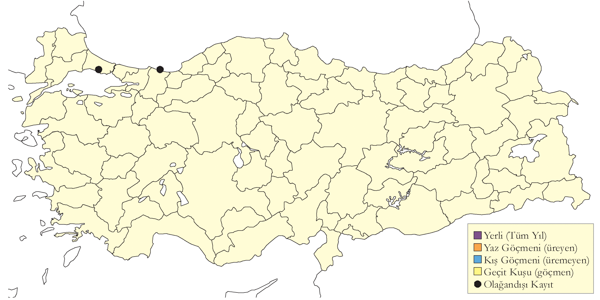
\includegraphics{images/harita_Page_006.png}

\hypertarget{uxfcreme-5}{%
\subsection{\texorpdfstring{\textbf{Üreme}}{Üreme}}\label{uxfcreme-5}}

Türkiye'de yuvalamaz. Grönland, İzlanda, Kuzey Batı Rusya ve Baltık
Denizi kıyılarında yuvalar.

\textbf{Alttürler ve Sınıflandırma}

Monotipik bir türdür.

\hypertarget{sibirya-kazux131}{%
\section{Sibirya Kazı}\label{sibirya-kazux131}}

\emph{Branta ruficollis}, Red-breasted Goose

\textbf{\emph{Az sayıda gelen düzensiz kış konuğudur.}}

Özellikle soğuk kışlarda bazı bireyler veya gruplar Türkiye'ye inerler
ve düzensiz olarak görülürler. Türkiye'de düzenli kışladığı bir alan
yoktur. Ana kışlama alanı Romanya ve Bulgaristan'ın Karadeniz kıyı
şerididir. 1964 ila 2008 arasında 64 kaydı bilinir. Bu kayıtların
Marmarada 15 kayıt, İç Anadolu'da 12 kayıt, Karadeniz'de 8 kayıt,
Akdeniz'de 6 kayıt ve Ege'de 4 kayıt alınmıştır. Kayıtların çoğu aralık
sonu ile şubat başı arasından gelir. Bu kayıtların çoğunda bir veya
birkaç kuş sayılmışi ancak 5 tanesinde 40 ila 100 bireylik kalabalık
sürüler de gözlenmiştir. 2001/2002 kışında ülke toplamında 192 birey
sayılmıştır.

Ülke genelinde yaygın olarak av mağazaları ve avcılık kulüplerinde
tahnitlerine rastlanması ve avcıların gözlem
beyanları\textsuperscript{24} kayıtların işaret ettiğinden çok yaygın
olduğunu gösterir. İç Anadolu'dan gelen eski kayıtlar, Kış Ortası Su Kuş
Sayımlarında kalabalık kaz sürülerinin sistematik incelenmesi ile ortaya
çıkmıştır. Sakarca sürülerinin içinde olabilecek bireylerin farkedilmeme
ihtimali yüksektir.

1946/47 kışında Küçükçekme'de Kosswig tarafından
gözlenmiştir\textsuperscript{23}. 1947 veya 1954 yılında kış boyunca (27
Kasım - 6 Mart) Büyükçekmece ve Meriç Nehri (?) arasında düzenli olarak
9 birey ve Beylik Mandra'da 2 birey kaydedilmiştir\textsuperscript{18}.
1959 yılında belirtilmemiş bir alanda sekiz İshakoğlu tarafından birey
gözlenmiş ve bir birey vurulmuştur\textsuperscript{25}. 12 Kasım 1964'de
Kuyucuk Gölü'nde 2 erişkin ve bir genç birey 400 boz kazın arasında
kaydedilmiştir\textsuperscript{26}. 17 Ocak 1965 tarihinde Çekmece'de E.
Hirzel tarafından üç birey görülmüştür.

Türkiye'den açıklamaya ihtiyaç duyulan bir yaz veya üreme kaydı vardır.
5 Ağustos 1982'de Erçek Gölü'nde 14 erişkin ve sekiz yavru
kaydedilmiştir\textsuperscript{27}. Bu kayıt ya hatalı bir kayıt olarak
unutulmalı, ya da avcılar tarafından yakalanmış ve evcilleştirilmiş
kuşların üretilmesinin bir sonucu olarak yorumlanmalıdır.

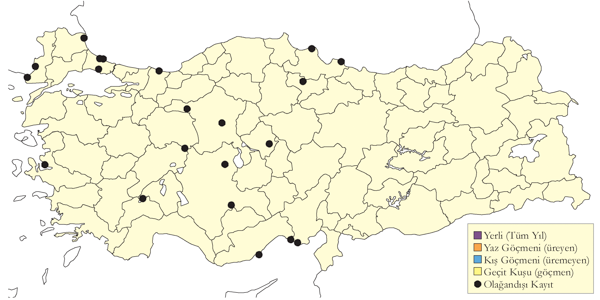
\includegraphics{images/harita_Page_007.png}

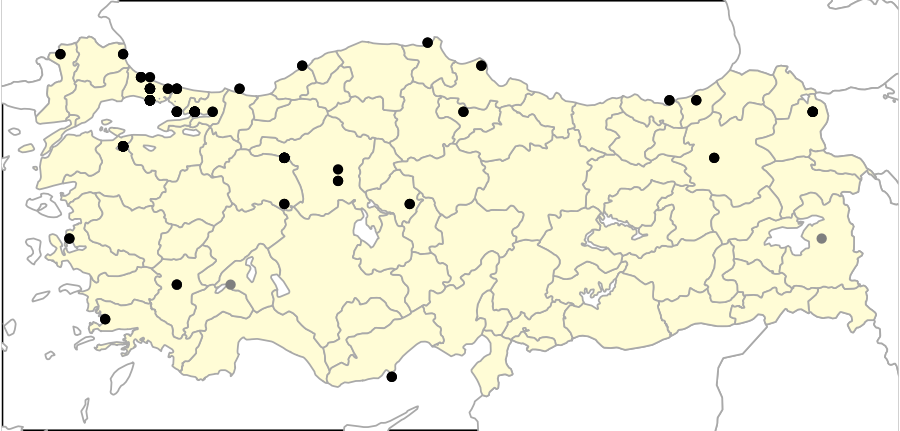
\includegraphics[width=6.25in,height=\textheight]{images/harita_Branta_ruficollis.png}

\hypertarget{uxfcreme-6}{%
\subsection{\texorpdfstring{\textbf{Üreme}}{Üreme}}\label{uxfcreme-6}}

Türkiye'de yuvalamaz. Doğu Sibirya'da tundra kuşağında yuvalar.

\textbf{Alttürler ve Sınıflandırma}

Monotipik bir türdür.

\hypertarget{sessiz-kuux11fu}{%
\section{Sessiz Kuğu}\label{sessiz-kuux11fu}}

\emph{Cygnus olor}, Mute Swan

\textbf{\emph{Lokal olarak az sayıda yuvalar. Yaygın olarak ve nispeten
çok sayıda bulunan bir kış konuğudur.}}

Üreme kayıtlarının çoğu 3 alandan gelir: Gala Gölü, Gediz Deltası ve
Kızılırmak Deltası. Ulusal üreme popülasyonu muhtemelen 20 çiftten daha
azdır. Kızılırmak Deltası'ndan ilk muhtemel üreme kaydı 1968 yılında
alınmıştır\textsuperscript{24}.

Geçmişte birkaç alanda üreyen yüzlerce çiftlik bir nüfus bulunuyordu.
Marmara Gölü'nde 50 çift, Akşehir Gölü'nde 100 çift
üremiştir\textsuperscript{28}. Ereğli Sazlığı en çok gözlem kaydının
alındığı alandır. Lenz burada 1968'de 11 yuva, 1969'da bir yuva ve
1970'de üç yuva bulmuştur. Buradaki sulakalanın yokolması ayrıntılı
olarak belgelendiği için\textsuperscript{29}, üreyen nüfusun azalışı da
gözlenmiştir. Eski üreme alanlarında yok olmasının ana nedeni
sulakalanların kurutulmasıdır.

Kışın Karadeniz ve Marmara ve Ege Bölgesinde yaygın olarak en yüksek
sayılarda gözlenir. Toplam kışlama popülasyonu 1000-10000 birey
arasındadır. Meriç Deltası ve Gala Gölü ülke nüfusunun çoğunun
toplandığı alandır, burada 1993'de 1244 birey\textsuperscript{12}
1999'da 8900 birey\textsuperscript{13} ve 2003'te 2000 birey
sayılmıştır. Kışın sert geçtiği yıllarda sayısı artar, 1999'da ülke
toplamında 9088 birey kaydedilmiştir.

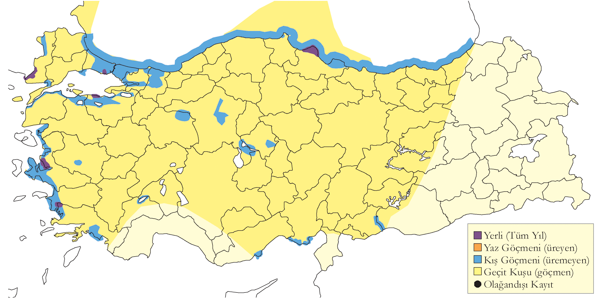
\includegraphics{images/harita_Page_008.png}

\hypertarget{uxfcreme-7}{%
\subsection{\texorpdfstring{\textbf{Üreme}}{Üreme}}\label{uxfcreme-7}}

\textbf{Yuvalama alanı:} Geniş sazlık alanlar ve göl açıklığı bulunan
büyük göller ve bataklıklardır.\\
\textbf{Yuvası:} Türkiye'deki bir yuvanın tarifi yapılmamıştır. Diğer
yerlerde yuva su kenarında zemin üzerinde, küçük bir adacıkta veya sığ
sudaki sazların üstüne kurulur. Yuva saz ve diğer sucul bitkilerden
oluşan büyük bir yığının ortasındaki çukura kurulur.\\
\textbf{Yumurta sayısı:} Türkiye'de yumurta gözlemi yoktur. Türkiye
dışında 5-7 yumurta koyduğu bilinir.\\
\textbf{Üreme dönemi:} Nisan başında yumurta koyar, mayıs ve temmuz
arasında yavrular gözükür. 13 Mayıs 1899'da İzmir'de saz yatağında
yuvalan bir çift kaydedilmiştir\textsuperscript{30}. 6 Temmuz 1976'da
Ereğli Sazlığında bir çift ve 4-5 genç yavru, 17 Temmuz 1982'de bir çift
ve dört genç ve 16 Mayıs 1987'de yumurtadan yeni çıkmış yavrular
gözlenmiştir.

\textbf{Alttürler ve Sınıflandırma}

Monotipik bir türdür.

\hypertarget{kuxfcuxe7uxfck-kuux11fu}{%
\section{Küçük Kuğu}\label{kuxfcuxe7uxfck-kuux11fu}}

\emph{Cygnus columbianus}, Tundra Swan

\textbf{\emph{Lokal olarak ve az sayıda bulunan bir kış konuğudur.}}

1993 yılına kadar nadir bir kış konuğu olduğu düşünülmüştür. Daha sonra
ilk önce Burdur Gölü ve Göller bölgesinde, ardından Meriç Deltası düzenl
bulunduğu tespit edilmiştir. Meriç Deltası'nda karışık ve kalabalık kuğu
sürüleri içinde sayıları 1000'e ulaşabilir. İç Anadolu, Göller
Bölgesi'nda küçük gruplar halinde bulunur. Ekseriyetle kasım ve nisan
arasında bulunur.

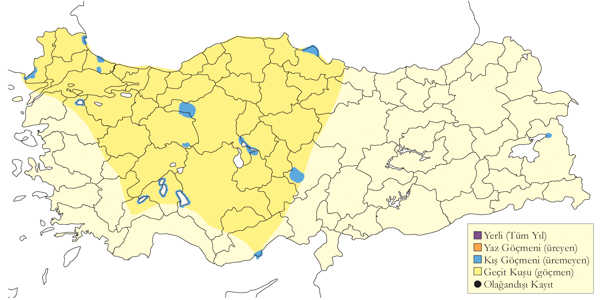
\includegraphics{images/harita_Page_009.png}

\hypertarget{uxfcreme-8}{%
\subsection{\texorpdfstring{\textbf{Üreme}}{Üreme}}\label{uxfcreme-8}}

Türkiye'de yuvalamaz. Türkiye'de kışlayan kuşların üreleme alanının ve
göç koridorları tespit edilmiştir\textsuperscript{31}. GPS ve GMS
vericileri ile 2015-2017 yılında yapılan çalışmada yuvalama alanlarının
Yamalo-Nenets özrek bölgesindeki Yamal olduğu, göçleri sırasında Ob
Koyu, Turgay Ovaları, Kuzey Hazar Kıyıları, Azov Denizi gibi durak
alanlar üzerinden göç ettikleri ortaya çıkmıştır.

\textbf{Alttürler ve Sınıflandırma}

Ülkemizde Eski Dünya'da yaşayan \emph{bewickii} alttürü bulunur ve gaga
kökü ve yüz derisi sarıdır. Amerika'da yaşayan \emph{columbianus}
alttürü siyah gaga ve siyah yüz derisi ile kolaylıkla ayırt edilebilir.

\hypertarget{uxf6tuxfccuxfc-kuux11fu}{%
\section{Ötücü Kuğu}\label{uxf6tuxfccuxfc-kuux11fu}}

\emph{Cygnus cygnus}, Whooper Swan

\textbf{\emph{Yaygın olarak ve az sayıda görülen bir kış konuğudur.}}

Ekim sonu ve nisan başı arasında yaygın olarak az sayıda görülen bir kış
konuğudur. Ocak ve şubat aylarında en yüksek sayıya ulaşır. Trakya'da
Meriç Deltası ana toplama bölgesi ve türün Balkanlar'daki en önemli
kışlama alanıdır. 25 Ocak 1998'de bulunan 1200 birey Türkiye'deki en
yüksek sayıdır.\textsuperscript{32} Türkiye'ye gelen kuşlar Ukrayna ve
Kırım ile Batı Karadeniz Bölgesi arasındaki deniz üzeri göç rotasını
kullanır\textsuperscript{33}. Doğuda 30 Ekim 1995'de Sodalı Gölü'nde 164
birey\textsuperscript{34}, 1992'de Diyarbakır Kabaklı Barajı'nda 133
birey\textsuperscript{35} kaydedilmiştir.

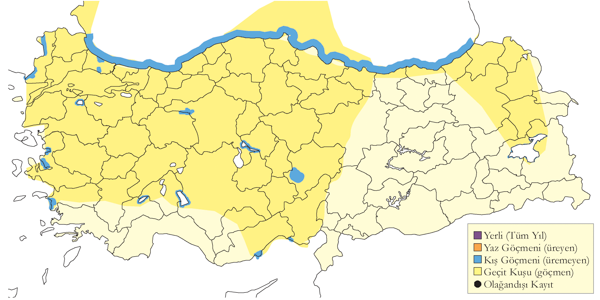
\includegraphics{images/harita_Page_010.png}

\hypertarget{uxfcreme-9}{%
\subsection{\texorpdfstring{\textbf{Üreme}}{Üreme}}\label{uxfcreme-9}}

Türkiye'de yuvalamaz. Avrasya'nın kuzeyinde yuvalar.

\textbf{Alttürler ve Sınıflandırma}

Monotipik bir türdür.

\hypertarget{nil-kazux131}{%
\section{Nil Kazı}\label{nil-kazux131}}

\emph{Alopochen aegyptiaca}, Egyptian Goose

\textbf{\emph{Durumu belirsizdir. Çoğunlukla egzotik tür kategorisinde
olsa da bazılarının rastlantısal konuk olma olasılığı vardır.}}

28 Nisan 1986'da Kulu Gölü'nde bir birey gözlenmiş, kuşun doğal ve
rastlantısal konuk olduğu düşünülmüştür. 11 Nisan 1911'de Urfa'nın
güneyinde iki birey gördüğünü söyleyen Weigold'un (1912-13) kaydı ise
kabul görmemiştir\textsuperscript{36}.

İstanbul ve Ankara'da gözlenen kuşların esaretten kaçtığı düşünülür.
6-13 Temmuz 2002'de Ankara'daki bir parkta bir çift fotoğraflanmış, 31
Mart 2012'de İstanbul Riva'da bir çift, 13 Mart 2012'de Ankara Hacettepe
Kampüsü'nde, 5-24 Kasım 2013'de Etimesgut'ta ve 25 Mayıs-13 Haziran
2014'da Eymir Gölü'nde birer birey gözlenmiştir.

1906 ve 1928 arasında Kıbrıs'ta nadir rastlanan bir kış göçmeni olarak
değerlendirilmiş, 1958, 1962 ve 1989 yıllarında bireyler gözlenmiştir.
Eskiden Suriye ve Filistin'de ürediğini düşünülmüş\textsuperscript{37},
sonrasında Suriye'de hiçbir güvenilir kaydı olmadığına karar
kılınmıştır\textsuperscript{38,39}.

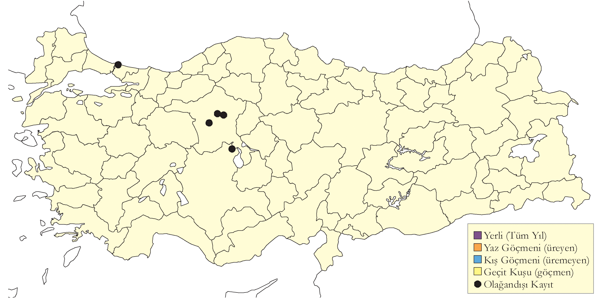
\includegraphics{images/harita_Page_011.png}

\hypertarget{uxfcreme-10}{%
\subsection{\texorpdfstring{\textbf{Üreme}}{Üreme}}\label{uxfcreme-10}}

Türkiye'de yuvalamaz. Afrika'da çoğunlukla Sahra Altında yuvalar.

\textbf{Alttürler ve Sınıflandırma}

Monotipik bir türdür.

\hypertarget{suna}{%
\section{Suna}\label{suna}}

\emph{Tadorna tadorna}, Common Shelduck

\textbf{\emph{Lokal olarak az sayıda ürer ve yaygın olarak çok sayıda
bulunan bir kış konuğudur.}}

Ege Bölgesi, Göller Bölgesi, İç ve Doğu Anadolu'da geniş ve tuzlu
sulakalanlarda ürer. Başlıca üreme alanları Gediz Deltası, Bolluk, Kulu
ve Tuz Gölleri ve Van Gölü çevresidir. Gediz Deltası'nda 1996 yılında
üreyen popülasyonun 8 çift olduğu tahmin edilmiş\textsuperscript{40}. 24
Haziran 1992'de Bolluk Gölü'ndeki bir adada 12 yuva bulunmuştur.

Üreme sonrası tüy değiştiren kuşlar ağustos-ekim arasında toplanırlar,
Erçek Gölü'nde 2500 birey, Kulu Gölü'nde 700 birey sayılmıştır.

Kışlayan toplam nüfus genellikle 1000-5000 bireydir, ana kışlama alanı
Yumurtalık Lagünü'nde 16 Şubat 2006'da 5390 birey sayılmıştır. Acıgöl'de
1969-70'de 3450 birey, 1968-69'da 4900 birey, 2004'te 1802 birey ve
2005'te 2928 birey sayılmıştır. Diğer alanlarda daha küçük topluluklar
oluşturur.

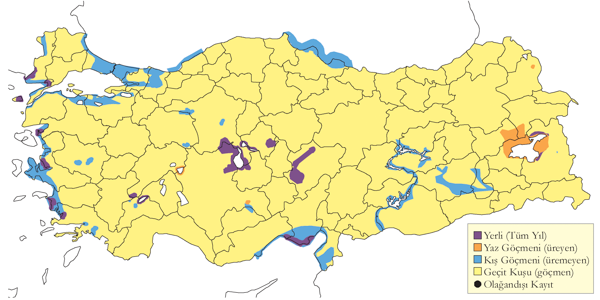
\includegraphics{images/harita_Page_012.png}

\hypertarget{uxfcreme-11}{%
\subsection{\texorpdfstring{\textbf{Üreme}}{Üreme}}\label{uxfcreme-11}}

\textbf{Yuvalama alanı:} Geniş, sığ ve tuzlu sulakalanlarda adalar,
sedde duvarları ve çalı altlarında yuvalar.\\
\textbf{Yuvası}: Avrupa'da yuvaların çoğu tavşan oyuklarında, tünelin
1-2 m içinde bulunur. Buna karşın Türkiye'deki yuvalar yerdedir. Bolluk
Gölü'ndeki yuvaların bazıları tamamen açıkta, bazıları kısmen ya da
tamamen çalı altında ve bir tanesi doğal bir oyuğun içinde
bulunmuştur.\\
\textbf{Yumurta sayısı:} 6-9 yumurta koyduğu gözlenmiştir. Bolluk
Gölü'ndeki yuvalarda gözlenen 10-18 yumurtanın birden çok dişi
tarafından konulmuş olması muhtemeldir.\\
\textbf{Üreme dönemi:} Gediz Deltasında haziran başında yavrular
görülmüştür\textsuperscript{40}. İç Anadolu'da nisan sonu ile haziran
başında yuvalar. Doğu Anadolu'da haziran ortasında yumurtladığı
düşünülmektedir.

\textbf{Alttürler ve Sınıflandırma}

Monotipik bir türdür.

\hypertarget{angux131t}{%
\section{Angıt}\label{angux131t}}

\emph{Tadorna ferruginea}, Ruddy Shelduck

\textbf{\emph{Yaygın ve çok sayıda bulunan yerli türdür. Kışın göç alır,
sayıları artar.}}

Üremek için Genellikle yüksek kesimlerdeki küçük gölcükler, baraj
gölleri, ıslak çayırlar ve dereleri seçer, birçok ördek ve kaz türünün
aksine büyük sulakalanlarda bulunmaz. İlk tahminde üreyen popülasyonun
4000 ile 8000 çift arasında olduğu öne sürmüştür\textsuperscript{41}.
Sonrasında kış ortası su kuşu sayımlarına dayanarak azaldığı
düşünülmüştür. Üreyen popülasyonun 1200-5100 çift olduğunu tahmin
etmiştir\textsuperscript{42}.

Temmuz eylül arasında tüy değişimi için bazı sulakalanlarda büyük
sürüler halinde toplanır. Erçek Gölü'nde 20.000 birey, Sultan
Sazlığı'nda 11.000 birey, Kulu Gölü'nde 10.000 birey, Eylül 1936'da
bugün kurutulmuş olan Emir Gölü'nde 10.000-15.000 birey sayılmıştır. Kış
öncesinde Kasım 2004'de Sarıyar Barajı'nda 8.000 birey ve Kuyucuk
Gölü'nde 6.000 birey kaydedilmiştir.

Kış aylarında daha yaygın olarak görülür. En yüksek kış sayımında ülke
toplamında 10.115 birey\textsuperscript{14}, genellikle 4000-4500 birey
sayılmıştır. Ocak-Şubat 1993'te sadece 711 birey, sadece Sarıyar
Barajı'nda 18 Ocak 2004'te 5636 birey ve 18 Şubat 2006'da 7641 birey
kaydedilmiştir. Bir yandan İç Anadolu'da üreme sonrası toplanan
sürülerde bir azalma görülmüş, diğer yandan baraj göllerinin sayısındaki
artış gözlenmiştir. Kış sayımı toplamlarının yaz sonu toplamlarından az
olması, dağınık şekilde kışladığına veya kış ayında güneye göç vermesine
bağlanabilir. Toplam kışlayan nüfusun 2600 ile 28.500 birey arasında
değiştiği düşünülmüştür\textsuperscript{42}.

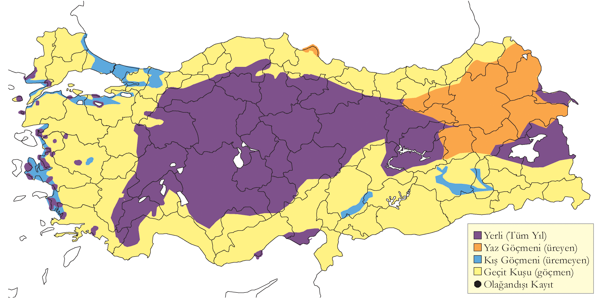
\includegraphics{images/harita_Page_013.png}

\hypertarget{uxfcreme-12}{%
\subsection{\texorpdfstring{\textbf{Üreme}}{Üreme}}\label{uxfcreme-12}}

\textbf{Yuvalama alanı:} Genellikle göl kenarlarındaki sarp kayalıklarda
ve tepelerde, yamaçlardaki çukur ve çatlaklarda olmak üzere açık
alanlarda ürer. Sıkça kayalıklarda yuvalar. Beyşehir Gölü'ndeki bir
adada kayaların ve harabelerin taşları arasında ürediği kaydedilmiştir.
22-24 Mayıs 1998'de Ereğli yakınlarındaki bir kayalıkta muhtemelen eski
bir Kızıl Şahin yuvasında kuluçkaya yatmış bir dişi gözlenmiştir.\\
\textbf{Yuvası}: Yuvası Türkiye'de tanımlanmamıştır, genellikle bitki
artıkları, hav tüyleri ve bazı diğer tüylerle kaplanmış bir oyuktur. 30
Nisan 2003'te Akköy yakınındaki dik bir yamaçtaki muhtemelen bir tavşan
yuvası olan oyuğa giren bir dişi gözlenmiş, ancak oyuğun derin olması
nedeniyle yuva incelenememiştir.\\
\textbf{Yumurta sayısı:} 8-12 yumurta koyduğu görülmüştür.\\
\textbf{Üreme dönemi:} Akdeniz ve Ege'de mart sonu yumurta koyar.
Kuluçka diğer bölgelerde nisan ve mayıs arasında başlar.

\textbf{Alttürler ve Sınıflandırma}

Monotipik bir türdür.

\hypertarget{boz-uxf6rdek}{%
\section{Boz Ördek}\label{boz-uxf6rdek}}

\emph{Mareca strepera}, Gadwall

\textbf{Lokal olarak birkaç alanda yuvalar. Yaygın olarak orta sayılarda
bulunan bir kış konuğudur.}

En önemli üreme alanı Kızılırmak Deltası'nda 200 çift ürer. Türkiye'de
toplam üreyen popülasyonun 500 ile 5000 çift arasında olduğu
düşünmüştür\textsuperscript{41}. Bugüne gelindiğinde sayılarının
azaldığı ortadadır.

İç Anadolu'daki ilkbahar geçişi marttan nisan başına kadar belirgindir.
Akdeniz'deki kıyısal sulakalanlarda nadiren 1000'den yüksek sayılarda
gözlenir. Kış ortası sayımlarda 1967'de Manyas Gölü'nde 5000 birey,
1969'da Akşehir Gölü'nde 7500 birey ve 1971'de Hotamış Sazlığı'nda 2490
birey sayılmıştır. 1967-73 arasında ülke genelinde çoğunlukla 3000'den
fazla kaydedilmiştir. 1986-2005 arasında toplam sayı 1000-1500
seviyesine düşmüş, son yıllarda tekrar artmış, 2020 kışında Kızılırmak
Deltası'nda 10.000 bireyden fazla sayılmıştır.

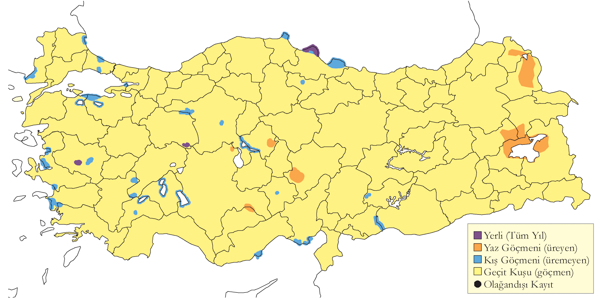
\includegraphics{images/harita_Page_014.png}

\hypertarget{uxfcreme-13}{%
\subsection{\texorpdfstring{\textbf{Üreme}}{Üreme}}\label{uxfcreme-13}}

\textbf{Yuvalama alanı:} Göl kıyılarında ve adalarındaki yoğun
vejetasyon içinde; sazlıklarda ve sık bitkilerle kaplı taşkın
alanlarında ürer. Kızılırmak Deltası, Karamık Gölü, Kulu Gölü, Bolluk
Gölü, Mogan Gölü, Ahlat Sazlıkları, Haçlı Gölü ve Van Gölü'nde
yuvalamıştır.\\
\textbf{Yuvası:} Yuva yerde bir çukura kurulur, bitkisel malzeme ve
dişinin tüyleriyle kaplanır. \textbf{\hfill\break
Yumurta sayısı:} Türkiye'deki yuvalarda yumurta sayısı 6-15 arasındadır.
İç Anadolu'da 7-15 yumurtalı yuvalar görülmüş, bu yumurtaların 1 ila 6
tanesi başka ördeklerin koymuş olduğu tespit edilmiştir. Kulu Gölü'ndeki
yuvalarda 6 Mayıs 1972'de 3-11 yumurta ve 14 Temmuz 1971'de 7 yumurta
sayılmıştır\textsuperscript{43}. 17 Mayıs 2004'te Bolluk Gölü'ndeki bir
yuvada 8 yumurta bulunmuştur.\\
\textbf{Üreme dönemi:} Kızılırmak Deltası'nda nisan başında yumurta
koyar\textsuperscript{44}. İç Anadolu'da nisan sonu ile temmuz arasında,
Doğu Anadolu'da haziran ile eylül arasında yavrulara rastlanmıştır.

\textbf{Alttürler ve Sınıflandırma}

Türkiye'de nominat alttürü bulunur. Eskiden \emph{Anas} cinsi altında
sınıflandırılırdı.

\hypertarget{fiyu}{%
\section{Fiyu}\label{fiyu}}

\emph{Mareca penelope}, Eurasian Wigeon

\textbf{\emph{Yaygın olarak çok sayıda bulunan kış konuğu ve geçit
türüdür.}}

Ege, Akdeniz ve İç Anadolu'nun sulakalanlarında kalabalık sürüler
halinde kışlar. 1960'lı ve 70'li yıllarda düzenli olarak ortalama
150.000 birey sayılmıştır. En yüksek sayıda 1968'de 208.600 birey,
1969'da 458.800 birey kaydedilmiştir. Bugünlere gelindiğinde ciddi bir
düşüş yaşamıştır. 1986 ile 2005 arasındaki düzenli sayımlarda sadece
dört yıl 40.000'dan fazla birey kaydedilmiştir. Çoğunlukla eylül sonunda
gelir, nisan sonuna kadar kalır.

İç Anadolu'da mart sonu ve nisan başı arasında yüksek sayıda geçer. Bazı
göçmenler mayıs sonuna kadar kalır. Nadiren Doğu Anadolu'da ve
muhtemelen İç Anadolu'da üremeden yazı geçirebilir.

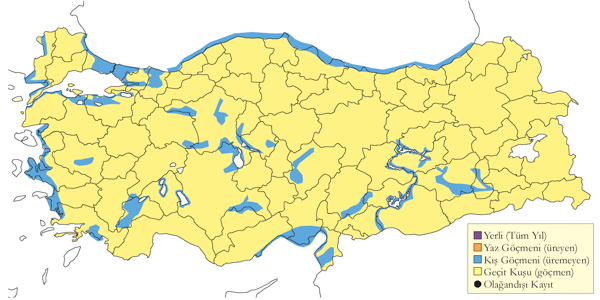
\includegraphics{images/harita_Page_015.png}

\hypertarget{uxfcreme-14}{%
\subsection{\texorpdfstring{\textbf{Üreme}}{Üreme}}\label{uxfcreme-14}}

Türkiye'de yuvalamaz. Kuzey Avrupa'da yuvalar.

\textbf{Alttürler ve Sınıflandırma}

Monotipik bir türdür. Eskiden \emph{Anas} cinsi altında
sınıflandırılırdı.

\hypertarget{yeux15filbaux15f}{%
\section{Yeşilbaş}\label{yeux15filbaux15f}}

\emph{Anas platyrhynchos}, Mallard

\textbf{\emph{Yaygın olarak üreyen yerli bir türdür. Kışın göç alır,
yüksek sayılara ulaşabilir.}}

Uygun yaşamalanının bulunduğu coğrafyalarda yaygın olarak az sayıda
yuvalar. En yaygın olarak İç Anadolu Bölgesi sulakalanlarında rastlanır,
diğer bölgelerde çok lokal olarak bulunabilir. En yüksek sayıda
yuvaladığı alan 400-600 çiftin kaydedildiği Kızılırmak Deltası
olmuştur\textsuperscript{44}.

Sonbaharda göç alır ves sayıları artar. Kışlayan gruplar nisan başına
kadar kalır. En yüksek sayılarda Karadeniz, Marmara ve Ege sahil
kuşağında kaydedilir. Akdeniz ve İç Anadolu'da nispeten az sayıda,
Güneydoğu Anadolu ve Doğu Anadolu'da az sayıda bulunur. 2000 ve 2020
arasında kışlayan nüfus ortalama 20.000 birey seviyesinde olsa da, kışın
soğuk geçtiği 2005 yılında ülke genelinde toplam 106.140 birey ve
Kızılırmak Deltası'nda 50.000 birey sayılmıştır.

1960 ve 70'li yıllarda kışlayan nüfusun 100.000'ler seviyesinde
olmuştur. 1967'de Kızılırmak Deltası ve Yeşilırmak Deltası'nda yaklaşık
52.000 ve Büyük Menderes Deltası'nda 42.000, 1968'de Manyas ve Uluabat
göllerinde 42.000, 1969'da Büyük Menderes Deltası'nda 80.000, Akyatan
Lagünü'nde 40.000 ve Amik Gölü'nde 30.000, 1970'de Meriç Deltası'nda
34.500 ve Sultansazlığı'nda 30.000 birey sayılmıştır.

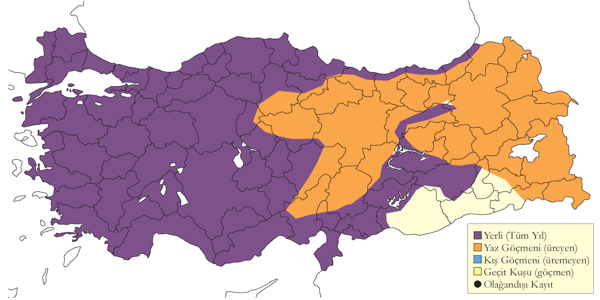
\includegraphics{images/harita_Page_016.png}

\hypertarget{uxfcreme-15}{%
\subsection{\texorpdfstring{\textbf{Üreme}}{Üreme}}\label{uxfcreme-15}}

\textbf{Yuvalama alanı}: Göl ve nehirlerdeki adacıklarda, sazlıklarda,
veya göl, sazlık veya subasar çayırların kıyılarındaki sık bitkilerin
içinde ürer.\\
\textbf{Yuvası}: Yuvasını genellikle bitki örtüsünün altına, topraktaki
bir oyuğa kurar. Başka bölgelerde ağaç kovuğuna yuvaladığı veya
ağaçtaki, örneğin karga gibi, bir kuş yuvasını kullandığı bilinir. Bu
tip yuvalara Türkiye'de henüz rastlanmamıştır.\\
\textbf{Yumurta sayısı}: Genellikle 5-9 yumurta koyar, ancak yumurta
sayısı 2-14 arasında olabilir. Bir yuvadaki yumurtaların 14'ten fazla
olması, birden fazla dişinin aynı yuvaya yumurtladığını gösterir.\\
\textbf{Üreme dönemi}: Kıyı bölgelerinde marttan itibaren, diğer
bölgelerde nisan veya mayısta yumurtlar. Yavrular mayıs başından temmuz
sonuna kadar görülebilir. \textbf{MAR.} 18 Nisan 1993'te Kocaçay
Deltası'nda yavrularıyla gözlenen bir dişi en erken üreme
kaydıdır\textsuperscript{45}. \textbf{KAR.} 19-20 Mayıs 1992'de Yeniçağa
Gölü'nde hem yuvadaki yumurtalar hem de yavrular gözlenmiştir. 5 Mayıs
1992'de Kızılırmak Deltası'nda ilk yavrular
gözlenmiştir\textsuperscript{44}. 16 Mayıs 1967'de Manyas Gölü'nde dokuz
yumurtalı bir yuva kaydedilmiştir. 20 Haziran 1973'te Trakya'da altı
yavrulu bir dişi gözlenmiştir. \textbf{İÇA.} 1971'de Yarma'daki birçok
yuvada diğer türlerin yumurtalarına rastlanmıştır, örneğin, bir yuvada
17 Yeşilbaş, üç Boz Ördek ve üç Macar Ördeği yumurtası tanınmıştır.
13-15 Temmuz 1971'de Kulu Gölü'nde sekiz yuva incelenmiş, yuvalarda 2-12
sayılmış\textsuperscript{43}, başka bir tarihte mayıs ve haziranda
yumurtalı yuvalar ve mayıs ortasından itibaren yavrular gözlenmiştir.
\textbf{DOA.} En erken kayıt 14 Haziran 1968'de Erçek Gölü'nde
kaydedilen yavrulardır. Aynı yerde, 28 Haziran 1968'de beş ve sekiz
yumurtalı iki yuva bulunmuş\textsuperscript{27} ve 9 Haziran 2001'de
Balık Gölü'nde yumurtalı iki yuva kaydedilmiştir.

\textbf{Alttürler ve Sınıflandırma}

Türkiye'de nominat alttürü bulunur.

\hypertarget{kaux15fux131kgaga}{%
\section{Kaşıkgaga}\label{kaux15fux131kgaga}}

\emph{Spatula clypeata}, Northern Shoveler

\textbf{\emph{Lokal olarak az sayıda yuvalar. Yaygın olarak çok sayıda
bulunan bir geçit türü ve kış konuğudur.}}

İç Anadolu ve Doğu Anadolu'daki birkaç büyük sulakalanda ve Kızılırmak
Deltası'nda yuvalar\textsuperscript{46}. 1970'lerde Kulu Gölü,
Kızılırmak Deltası bilinen üreme alanlarıdır.

Tüm bölgelerde yaygın ve bol olarak kaydedilen bir geçit türüdür. Göçmen
gruplar ilkbaharda mart başından nisan sonuna kadar ve sonbaharda eylül
ortasından kasım başına kadar zaman zaman yüksek sayılarda görülür.
Eylülde Kulu Gölü'nde 7000 birey, Sultansazlığı'nda 9000 birey, mart
sonunda Kızılırmak Deltası'nda 4500 birey sayılmıştır.

Ülkenin batı ve orta bölgelerinde kışlar. 2000 ile 2020 arasında toplam
kışlayan kuş sayısı çoğunlukla 5000 bireyden az olmuştur, kışın soğuk
geçtiği 2005'te 13.576 birey sayılmıştır. Eskiden daha yüksek sayılar
kışlardı, 1993'te toplam 7898 birey, 1999'da 13.114 birey
kaydedilmiştir. Geçmikteki yüksek sayımları şöyledir; 1967'de Büyük
Menderes Delta'sında 23.000 birey, Kızılırmak Deltası'nda 8000 birey,
1993'te aynı yerde 4564 birey ). 1967-73 yılları arasında İç
Anadolu'daki birçok alanda sayıları 3000'i bulan sürülerin kaydı
kaydedilmiştir.

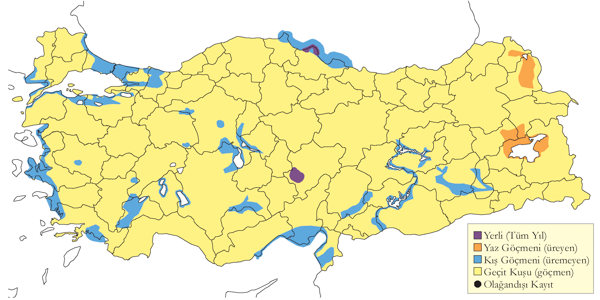
\includegraphics{images/harita_Page_017.png}

\hypertarget{uxfcreme-16}{%
\subsection{\texorpdfstring{\textbf{Üreme}}{Üreme}}\label{uxfcreme-16}}

\textbf{Yuvalama alanı}: Büyük sulakalanlarda yuvalar.\\
\textbf{Yuvası}: Kulu Gölünde bir adadaki cılız vejetasyonun içinde
yuvalamıştır. Çıplak zeminde sığ bir oyuğun içindeki yuva ot ve bitki
gövdeleri ile karışık olarak hav tüyleri ile kaplıdır.\\
\textbf{Yumurta sayısı}: 8-10 yumurta koyduğu kaydedilmiştir.\\
\textbf{Üreme dönemi}: Türkiye'de üremenin sezonu ile ilgili güvenle
yorum yapabilecek yeterli veri yoktur; diğer yerlerde üreme sezonunun
başlaması nisan başından mayıs sonuna kadar değişkenlik gösterebilir.
\textbf{KAR.} 6-7 Temmuz 1972'de Kızılırmak Deltası'nda dört ve beş
yavrulu iki dişi kaydedilmiş\textsuperscript{24}, 1992'de ürediği
kanıtlanamadığı için popülasyonun 0-1 çift olduğu tahmin
edilmiştir\textsuperscript{44}. 1971 Temmuz ortasına ait yumurtalı yuva
kayıtları başarısız bir üremenin ardından ikinci teşebbüs olarak
değerlendirilmelidir. \textbf{İÇA.} 14-15 Temmuz 1971'de Kulu Gölü'ndeki
bir adada sekiz ve on yumurtalı iki yuva bulunmuş, 5-6 Ağustos 1972'de
iki ve dört yavrulu iki yavru grubu görülmüştür\textsuperscript{43}. 31
Mayıs 1987'de Kulu Gölü'nde yavrular gözlenmiş ve 19 Haziran 1992'de
dokuz yumurtalı bir yuva bulunmuştur. Haziran 1977'de Eşmekaya'da beş
yavrusuyla birlikte bir dişi gözlenmiştir\textsuperscript{47}.
\textbf{DOA.} 29 Mayıs 1969'da Van Gölü'nde kur davranışı gözlenmiştir.

\textbf{Alttürler ve Sınıflandırma}

Monotipik bir türdür.

\hypertarget{kux131lkuyruk}{%
\section{Kılkuyruk}\label{kux131lkuyruk}}

\emph{Anas acuta}, Northern Pintail

\textbf{Nispeten yaygın olarak bulunan bir geçit türü ve kış konuğudur.
Nadiren yuvalar.}

Son yıllarda tek bir alanda yuvaladığı bilinir; 1998 ve 1999'da Girdev
Gölü'nde üremiştir. İlkbaharda ve yazın İç Anadolu'da birçok erişkin
kaydı olsa da, kanıtlanmış üreme kayıtları az sayıdadır. Üreyen
popülasyonun 500 ile 1000 çift olması iddiası tamamen
geçersizdir\textsuperscript{41}.

Genellikle eylül ortasından nisan başına kadar batı ve orta bölgelerinde
görülür. Geçit yapan kuşların görülme dönemleri ve sayıları hakkında bir
bilgi derlenmemiştir.

Ülke genelinde kışlayan nüfus 10.000 bireyden azdır. 1986'da toplam
25.700 birey, 1992'de 11.070 birey ve 1999'da 13.573 birey kışlamıştır.
Kışlama popülasyonunda çarpıcı bir azalma belgelenmiştir. 60'li yıllarda
düzenli olarak 100.000'in üzerindeki sayılarla kaydedilirdi. Örneğin,
1967'de Büyük Menderes Deltası'nda 60.000 birey, Emir Gölü'nde 70.000
birey, 1969'da Akyatan Gölü'nde 100.000 birey ve Gâvur Gölü'nde 50.000
birey kaydedilmiştir. Bilhassa ılıman geçen kışlarda daha yüksek
sayılarda kaydedilebilir. Eski tarihlerde bazı alanlardaki sayımların
sonuçlarının güvenilirliği sorgulanabilir, örneğin, 1970'de
Sultansazlığı'ndaki sayılan 160.000 birey muhtemelen abartılı bir
tahmindir. Bu ve diğer ördek türlerinin önemli sayılarda kışladığı
birkaç sulakalan kısmen ya da tamamen kurutulmuş durumdadır. Diğer
yandan son yıllarda oluşan baraj göllerinde kışlamaya başlamıştır.

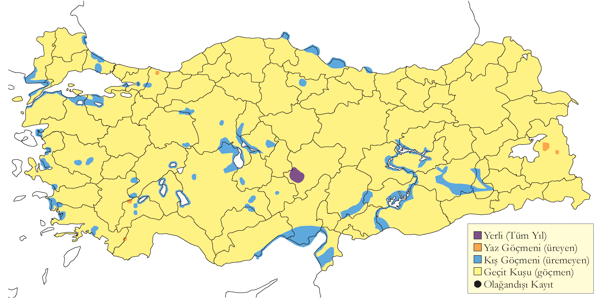
\includegraphics{images/harita_Page_018.png}

\hypertarget{uxfcreme-17}{%
\subsection{\texorpdfstring{\textbf{Üreme}}{Üreme}}\label{uxfcreme-17}}

\textbf{Yuvalama alanı}: Büyük göllerde ve sulakalanlarda yuvalar.\\
\textbf{Yuvası}: Kulu Gölü'ndeki büyük adanın kenarlarındaki
vejetasyonun içinde yuvalamıştır. Yerdeki bir delikte yaptığı yuvasını
bitkisel malzeme, hav tüyü ve biraz tüyle kaplar.\\
\textbf{Yumurta sayısı}: 6-10 yumurta koyduğu kaydedilmiştir.\\
\textbf{Üreme dönemi}: Görünüşe göre mayıs ayında yumurtlar.
\textbf{KAR.} Kızılırmak Deltası'nda üreme davranışları gözlense de
ürediği kesin olarak kanıtlanamamıştır\textsuperscript{44}.
\textbf{AKD.} Hem Haziran 1998 ve Haziran 1999'da Girdev Gölü'nde
yavrular gözlenmiştir. \textbf{İÇA.} 22 Mayıs 1992'de Kulu Gölü'nde yedi
ve on yumurtalı iki yuva, 19 Haziran 1992'de 6 ila 9 yumurtalı beş yuva
bulunmuştur. 24 Haziran 1992'de Bolluk Gölü'ndeki bir çalının altına
gizlenen yuvada 11 yumurta sayılmıştır.

\textbf{Alttürler ve Sınıflandırma}

Türkiye'de nominat alttürü bulunur.

\hypertarget{uxe7ux131krux131kuxe7ux131n}{%
\section{Çıkrıkçın}\label{uxe7ux131krux131kuxe7ux131n}}

\emph{Spatula querquedula}, Garganey

\textbf{Yaygın olarak az sayıda üreyen bir yaz göçmenidir. Göç döneminde
daha yaygın ve çok sayıdadır. Nadiren kışlar.}

Ördeklerin arasında esasen yaz göçmen olan tek türdür. Şubat ortasından
itibaren görülmeye başlar, ekim sonuna kadar kalır. Leylekle beraber en
erken gelen yaz göçmenlerindendir. Sazlık sulakalanları tercih eder, en
yoğun ürediği alanlar İç ve Doğu Anadolu'da bulunur. Güneydoğu
Anadolu'da potansiyel olarak iki üreme alanı tanımlanmıştır.

Göçmen sürülerin geçişi şubat sonundan mayıs sonuna kadar devam eder.
Hem ilkbaharda hem de sonbaharda tüm bölgelerde yüzlerce, hatta binlerce
bireylik sürüler halinde görülebilir. Ağustos sonu ve eylül başı
arasında Karadeniz kıyıları boyunca göçmen sürülere rastlanır.

Nadiren Marmara, Ege ve Akdeniz'de az sayıda kışlar. Olağandışı yumuşak
geçen 1968-69 kışında Göksu Deltası'nda 3000 birey ve Gâvur Gölü'nde
5000 birey sayılmıştır. Güncel tarihlerde; Ocak 2002'de Güllük
Deltası'nda 65 birey, Şubat 2002'de Bafa Gölü'nde 58 birey, Aralık
2002'de Çukurova'da 89 birey, 4 Aralık 2010'de Karkamış Barajı'nda iki
birey kışlamıştır.

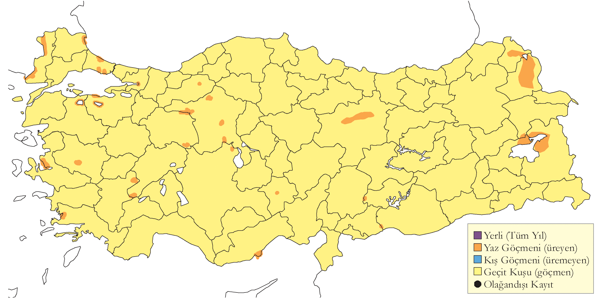
\includegraphics{images/harita_Page_019.png}

\hypertarget{uxfcreme-18}{%
\subsection{\texorpdfstring{\textbf{Üreme}}{Üreme}}\label{uxfcreme-18}}

\textbf{Yuvalama alanı}: Sazlık sulakalanlarda yuvalar.\\
\textbf{Yuvası}: Göl kenarlarındaki ıslak çayırlar, bataklıklar ve
sazlıklarda, ikisinin bir arada olduğu alanlarda ve göl kenarındaki
vejetasyonun içinde ürer.\\
\textbf{Yumurta sayısı}: Türkiye'den veri yoktur, diğer yerlerde olağan
yumurta sayısı 8-11'dir.\\
\textbf{Üreme dönemi}: Nisan ortasından itibaren ürer. Yavrular temmuza
kadar görülebilir. \textbf{KAR.} 19 Mayıs 1992'de Yeniçağa Gölü'nde yeni
bozulmuş ancak yumurtaların taze olduğu açıkça anlaşılan iki yuva, 6
Mayıs 1993'te yakınlardaki ıslak bir çayırlıkta bir yuva bulunmuştur. 13
Mayıs 1986'da Abant Gölü'nde 17 yavru ve bir dişi gözlenmiş, yumurtlama
tarihinin nisan ortası civarında olduğunu hesaplanmıştır. 2 Ağustos
1971'de Kızılırmak Deltası'nda bir çift ve yedi yavru kaydedilmiştir.
\textbf{İÇA.} 10-15 Mayıs 1991'de Hotamış Sazlığı'nda yavrulu birkaç
çift gözlenmiş\textsuperscript{48}, 27 Temmuz 1971'de Kulu Gölü'nde
büyük yavruları olan altı çift kaydedilmiş, Haziran ve Temmuz 1968'de
Mogan Gölü'nde 1-2 kuluçka gözlenmiş, 27 Temmuz 1971'de Yarma'da büyük
yavruları olan en az dört çift tespit edilmiştir.

\textbf{Alttürler ve Sınıflandırma}

Monotipik bir türdür.

\hypertarget{uxe7amurcun}{%
\section{Çamurcun}\label{uxe7amurcun}}

\emph{Anas crecca}, Eurasian Teal

\textbf{\emph{Lokal olarak az sayıda ürer. Yaygın olarak ve çok sayıda
bulunan kış konuğudur.}}

İç Anadolu, Doğu Anadolu bölgeleri ve Kızılırmak Deltası'nda yuvalar.
Delta'da 1992'de 15-20 çift üremiştir\textsuperscript{44}, Doğu
Anadolu'dan teyit edilmiş üreme kaydı çok azdır.

Geçiş sırasında eylül başından nisan başına kadar ülkenin batı ve orta
bölgelerinde yaygın olarak çok sayıda görülebilir. Marmara ve Karadeniz
bölgelerinde ara sıra yüksek sayılarda kaydedilebilir.

Kışın hem iç bölgelerde hem de kıyısal sulakalanlarda yüksek sayıda
bulunur. Ülke çapında kışlayan nüfus 100.000 birey seviyesindedir. Son
yıllarda kışlayan nüfusta düşüşler yaşanmış, örneğin 1988'de 21.000
birey ve 1989'da 13.400 birey sayılmıştır. Bu düşüş aslında diğer yüzey
ördeklerinde olduğu gibi 60'li yıllardan beri süre gelmektedir.
1968-69'da toplam 270.400 birey ve 1969-70'de 326.700 birey sayılmıştır.
Son sayımda sadece Sultansazlığında 200.000 birey gözlenmiştir. Alanda
sayılan ancak türü tespit edilemeyen 400.000 ördeğin de çamurcun
olabileceği düşünülürse alandaki kışlayan çamurcun sayısı 600.000 birey
olabilir.

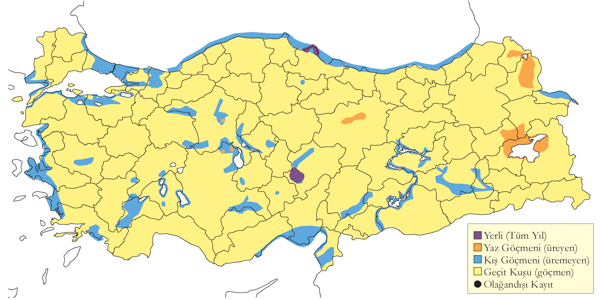
\includegraphics{images/harita_Page_020.png}

\hypertarget{uxfcreme-19}{%
\subsection{\texorpdfstring{\textbf{Üreme}}{Üreme}}\label{uxfcreme-19}}

\textbf{Yuvalama alanı}: Göllerde ve sazlıklarda ürer.\\
\textbf{Yuvası}: Yuva ve yumurta sayısı Türkiye'de tanımlanmamıştır.
Diğer yerlerde yerdeki bir oyuğa yaptığı yuvasını genellikle yapraklar,
bitkisel malzemeler, hav ve kontur tüyleriyle kaplar. Sulakalanlarda
yüksek otların üzerine yuvalar. Nadiren sudan uzağa yuva yapabilir.\\
\textbf{Yumurta sayısı}: Türkiye'den veri yoktur, diğer yerlerde olağan
yumurta sayısı 8-12'dir.\\
\textbf{Üreme dönemi}: Nisan ortasından itibaren ürer. Yavrular temmuza
kadar görülebilir. \textbf{KAR.} 29 Mayıs 1979'da Kızılırmak Deltası'nda
içinde yumurta olan bir yuva bulunmuş, 28 Temmuz 1971'de dokuz yavrulu
bir dişi, 6 Ağustos 1971'de beş yavrulu bir dişi
gözlenmiştir\textsuperscript{24}. 1992'de popülasyonun 15-20 çift olduğu
belirlenmiş, 5 Mayıs'ta dikkati farklı yere çekme davranışı gözlenmiş
ancak hiçbir yuva bulunamamıştır\textsuperscript{44}. \textbf{İÇA.} 14
Mayıs 1991'de Hotamış Sazlığı'nda yavrularıyla birlikte birkaç erişkin
gözlenmiş, buna göre yumurtaların en geç nisan ortasında koyulduğu
hesaplanmıştır\textsuperscript{48}. 5-6 Ağustos 1972'de Kulu Gölü'nde
iki dişinin 7 ve 10 yavrusu gözlenmiştir\textsuperscript{43}.
\textbf{DOA.} 24 Haziran 1983'te Haçlı Gölü'nde tek yavrulu bir dişi
kaydedilmiştir.

\textbf{Alttürler ve Sınıflandırma}

Türkiye'de nominat alttürü bulunur.

\hypertarget{yaz-uxf6rdeux11fi}{%
\section{Yaz Ördeği}\label{yaz-uxf6rdeux11fi}}

\emph{Marmaronetta angustirostris}, Marbled Duck

\textbf{\emph{Nadir yaz konuğudur.}}

Göksu Deltası'nda üreyen popülasyonun 2013 yılından sonra yokolmasıyla,
üreyen tür olarak soyunun tükendiği söylenebilir. Nadiren Güneydoğu
Anadolu'da görülebilir, Marmara, Ege ve Karadeniz bölgelerinde eski
tarihli kayıtları vardır. En yakın üreme alanı Irak'ta Mezopotamya
Bataklıkları'dır.

Mart başından ekim başına kadar kaydedilen bir yaz konuğu idi. Göksu
Deltası'nda üreyen popülasyon 1989 ile 2013 arasındaki adım adım
azalmıştır. 1989 ve 1991'de yaklaşık 50 çift tespit edilmiş, 2000'li
yıllarda 10 çifte düşmüş, 2010 ve 2013 arasında sadece 1 ila 2 çift
kalmış, 2014 yılından itibaren alanda görülmemeye başlamıştır. Bu
nedenle Türkiye'de üreyen nüfusunun yok olduğu kabul
edilmiş\textsuperscript{46} ve Yaz Ördeği Yılanboyun'dan sonra
Türkiye'de soyu tükendiği belgelenen kuş ilk türü olmuştur.

1987 yılında Çukurova'da bugün yok edilmiş olan Dipsiz Gölü'nde 32 çift
tespit edilmiştir. İç Anadolu'da Ereğli Sazlığı'nda muhtemelen 1-4 çift,
Hotamış Sazlığı'nda 10-15 çift, Sultansazlığı 1-4 çift üremiştir. Van
Gölü havzasında; Erciş Gölü ve Van Sazlığı'nda az sayıda ürediği teyit
edilmiş, bunun yanında Ağrı çevresi, Ahlat Sazlıkları, Bendimahi Deltası
ve Kuyucuk Gölü'nde üreme döneminde görülmüştür. 1987 yılında ülke
nüfusunun da 50-100 çiftin olduğu düşünülmüştür. Üreme sonrasında
Çukurova ve Göksu Deltasında 100-200 bireyin toplandığı bilinir. Nadiren
az sayıda kışlamıştır. En son sayımlarda 1993'te Çukurova'da dört,
1997'de aynı alanda 35 birey sayılmıştır.

Amik Gölü'nün kurutulmasında önce muhtemelen önemli sayılarda
bulunuyordu\textsuperscript{49}. Konya havzasında bulunan Yarma
Sazlıkları, Gönenç Gölü ve Karapınar Ovası'nda\textsuperscript{50}
muhtemelen üremiştir. Mogan Gölü ve Eber Gölü gibi diğer birkaç alanda
da muhtemelen üremiştir. Bu alanlar ekolojik özelliklerini kaybettikleri
ve türe uygun üreme habitatları barındırmadıkları için artık üremeye
elverişli değildirler. Üreme sonrası toplanan bireyler o yıllarda toplam
ülke nüfusu konusunda fikir verebilir. Ağustos 1967'de Çukurova'da 2000
birey ve Göksu Deltası'nda 450 birey sayılmıştır.

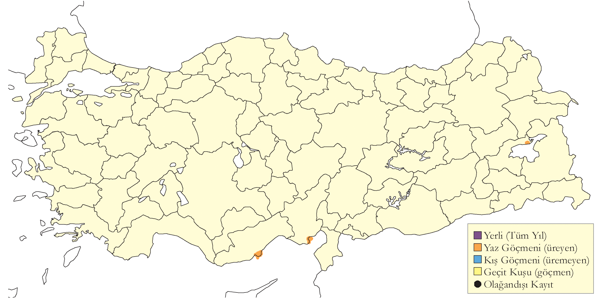
\includegraphics{images/harita_Page_021.png}

\hypertarget{uxfcreme-20}{%
\subsection{\texorpdfstring{\textbf{Üreme}}{Üreme}}\label{uxfcreme-20}}

\textbf{Yuvalama alanı}: Çukurova ve Göksu Deltası'nda sığ ve ötrofik
göllerde bulunmuştur. Genellikle sazlık adaların, bitişik havuzlar ve
sazlıkların bulunduğu yoğun sualtı vejetasyonuna sahip sığ göllerin
çevresinde ürer ve geniş sulakalanları tercih eder. Sanılanın aksine acı
veya tuzlu sularda değil, tatlı suları tercih eder.\\
\textbf{Yuvası}: 9 Haziran 1993'te Göksu'da, kofanın (\emph{Juncus})
baskın olduğu ve yakınlarda sazların (\emph{Phragmites}) da bulunduğu
bataklık bölgede sığ gölcüklerin olduğu bir alanda, yaklaşık 1 m.
çapındaki bir \emph{Juncus} kümesinin içinde, sudan yaklaşık 0,7 m
yüksekte iyice gizlenmiş bir şekilde yumurtaların henüz tamamlanmadığı
iki yumurtalı bir yuva bulunmuştur. Çok daha fazla yumurta için
yapıldığı açıkça belli olan, sazlardan ve bitki gövdelerinden yapılmış
dayanıklı ve derin bir kâse şeklindeki yuva daha ince bitkisel
malzemeyle kaplanmış, hiç hav tüyü kullanılmamıştır.\\
\textbf{Yumurta sayısı}: 2-12 arasında değişir, ortalama yumurta sayısı
6,5 olarak hesaplanmıştır\textsuperscript{51}. Başka yerlerdeki tipik
yumurta sayısı 9-13'tür (5-18).\\
\textbf{Üreme dönemi}: 22 Mayıs 1971'de Çukurova'da kaydedilen altı
yavru en erken kayıttır ve yumurtlamanın nisanın ikinci yarısında
başladığını gösterir. Ana yumurtlama dönemi mayısın ikinci yarısıyla
haziran başı arasındadır. Yavrular en erken 7 Haziran'da ortaya çıkarlar
ve temmuz sonuna kadar küçük yavrular görülebilir. Tamamen palazlanmış
yavrular temmuz başında kaydedilmiştir. \textbf{AKD.} 1991'de Göksu
Deltası'nda yaklaşık 50 çiftin en az 31'İ yavru çıkarabilmiştir. 1991'de
Göksu Deltasında 11 yuvada 8-13 yavru, 5 yuvada 4-6 yavru ve bir yuvada
15 yavru sayılmıştır. 15 yavrunun iki dişinin yumurtalarının bir araya
gelerek oluşturmuştur. Benzer şekilde 15-18 Temmuz 1992'de bir dişi 32
yavruyla görülmüştür\textsuperscript{51}. 10 Temmuz 1967'de kaydedilen
hem büyük hem de küçük yavrular az sayıda haziran ve daha çok temmuzda
gözlenmiştir\textsuperscript{52}. \textbf{İÇA.} 4-5 Haziran 1971'de
Yarma Sazlığı'nda 6 ve 13 yumurtalı iki yuva bulunmuş, bir yuvada bir
Yeşilbaş yumurtasına rastlanmıştır. 12 Haziran 1998'de Kulu Gölü'nde tek
yavrulu bir erişkin kaydedilmiş ve temmuzda üç farklı alanda yavrular
gözlenmiştir. \textbf{DOA.} 22 Temmuz 1987'de Van Sazlığı'nda küçük
yavruları olan iki çift gözlenmiş, bu gözleme göre yumurtlamanın haziran
ortasında olduğunu tahmin edilmiştir. Aynı alanda temmuz sonunda ve
ağustos başında genç bireyler kaydedilmiştir.

\textbf{Alttürler ve Sınıflandırma}

Monotipik bir türdür.

\hypertarget{macar-uxf6rdeux11fi}{%
\section{Macar Ördeği}\label{macar-uxf6rdeux11fi}}

Netta rufina, Red-crested Pochard

\textbf{\emph{Lokal olarak nispeten çok sayıda ürer. Kışın daha
yaygındır ve bazı alanlarda yüksek sayılarda toplanır.}}

İç Anadolu'daki geniş sodalı ya da tatlı sazlık sulakalanlarda çok
sayıda ürer. Sultansazlığı'nda yüksek sayıda bulunur. 1990'larıda Ereğli
Sazlığı'nda 500 çift, 1998'de sadece 20 çift üremiş, sonra alanın
kurutulmasıyla alandan yok olmuştur. Kızılırmak Deltası'nda 1992'de
50-75 çift üremiştir\textsuperscript{44}. Diğer alanlarda nispeten
yüksek sayılarda yuvalayanlar yerli veya yarı göçmendir. Çukurova
sulakalanları ve Göksu Deltası'nda üreyen nüfus 1990'dan sonra
azalmıştır. Türkiye'de üreyen popülasyon 1000-5000 çift olarak tahmin
edilmiştir\textsuperscript{41}. Son yıllarda İç Anadolu'da üreyen
kuşların sayılarında yaşanan azalma, güncel ulusal nüfusun çok daha az
olduğuna işaret eder. \footnote{Kerem Okudu 15 Haziran}

Ülke genelinde geçiş sırasında doğu bölgeleri dışında daha yaygındır.
Çoğu zaman yüzeyi donmaya daha az eğilimli olan baraj göllerini tercih
eder. Ocak 1967'de 12.000 birey sayılmış olup, bunun 7000 tanesi bugün
kurutulmuş Amik Gölü'ndendir. Türkiye genelinde 1992'de 5249, 1996'da
6522 ve 1999'da 6228 birey sayılmıştır. 2000'lı yıllarda toplam sayıda
artma görülmüş, sadece Beyşehir Gölü'nde Şubat 2003'te 10.000 birey ve
Ocak 2005'te 20.000 birey sayılmış, son sayımda hem toplam hem de alan
rekoru kırılmıştır.

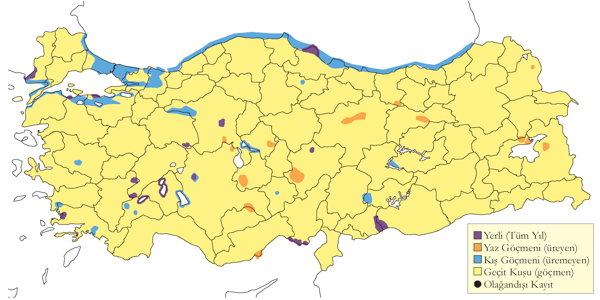
\includegraphics{images/harita_Page_022.png}

\hypertarget{uxfcreme-21}{%
\subsection{\texorpdfstring{\textbf{Üreme}}{Üreme}}\label{uxfcreme-21}}

\textbf{Yuvalama alanı}: Yoğun sazlıkların ve su kenarı bitkilerinin
bulunduğu tatlı ya da sodalı göllerde ve su aynalarına sahip sazlıklarda
ürer.\\
\textbf{Yuvası}: Yerdeki bir oyuğa yaptığı yuvasını bitkisel malzeme,
hav tüyleri ve tüylerle kaplar. Çoğunlukla yoğun vejetasyonun içine,
nadiren açıkta (örneğin adalarda) ya da nemli alanlarda su seviyesinin
üzerindeki saz öbeklerinin ya da diğer sucul bitkilerin içine genellikle
iyice gizlenmiş bir yuva yapar.\\
\textbf{Yumurta sayısı}: Türkiye'de gözlenen yumurta sayısı 4-12 olup,
ortalama 8,3'tür (18 yuvada). Bir yuvada bulunan 24 yumurta muhtemelen
birden fazla dişiye aittir. Yavru sayısı 2-12 arasında değişir, 16
yuvada ortalama 6,2'dir. Sadece 2-4 yavru çıkarabilmiş 6 dişi ortalamayı
düşürmüştür.\\
\textbf{Üreme dönemi}: Nisan sonu ile temmuz başı arasında yumurtlar.
Yavrular temmuz sonuna kadar görülebilir. \textbf{MAR.} 1 Mayıs 1993'te
Kocaçay Deltası'nda yumurtalı bir yuva bulunmuştur\textsuperscript{45}.
\textbf{KAR.} Kızılırmak Deltası'nda 27 Mayıs 1992'de beş yumurtalı bir
yuva bulunmuş, 4 Haziran 1992'de yaklaşık bir haftalık ilk tüylü yavru
kaydedilmiş\textsuperscript{44} ve 27 Mayıs 1979'da sekiz yavrulu bir
aile gözlenmiştir\textsuperscript{24}. \textbf{AKD.} 18 Temmuz 1992'de
Karamık Gölü'nde küçük yavrulardan oluşan bir aile gözlenmiştir.
\textbf{İÇA.} Çoğu mayısta olmak üzere 25 Nisan'da yumurta kayıtları
vardır. En geç kayıt 19 Haziran 1992'de 12 yumurtalı bir yuvadır. Biri
11 Mayıs'ta, çoğu haziranda olan birçok yavru kaydı vardır, en geç 8
Temmuz 1967'de\textsuperscript{52} ve 5 Ağustos 1972'de küçük yavrular
gözlenmiştir. \textbf{DOA.} 21-22 Temmuz 1986'da Van Gölü'nde 7-8
yavrulu üç yavrulu bir aile kaydedilmiştir.

\textbf{Alttürler ve Sınıflandırma}

Monotipik bir türdür.

\hypertarget{elmabaux15f-patka}{%
\section{Elmabaş Patka}\label{elmabaux15f-patka}}

\emph{Aythya ferina}, Common Pochard

\textbf{Nispeten yaygın ve çok sayıda bulunan yerli ve yarı göçmen,
yaygın ve çok sayıda bulunan kış konuğudur.}

İç ve Doğu Anadolu'daki sulakalanlarda orta sayılarda üreyen yerli ve
yarı göçmendir. 1992'de Kızılırmak Deltası'nda 300-350 çiftin ürediği
tahmin edilmiştir\textsuperscript{44}. Uygun habitatların azlığı
nedeniyle Karadeniz, Güneydoğu Anadolu ve belki de diğer bölgelerde
lokaldir. Muhtemelen gerçek üreme durumunu çarpıtacak şekilde hatırı
sayılır sayıda üremeyen birey özellikle İç ve Doğu Anadolu'da yazı
geçirir.

Kışın ve geçiş sırasında ülke genelinde yaygın ve boldur. Son yıllarda
ortalama 67.000 bireyden fazla sayılmaktadır. 1996 yılında Beyşehir
Gölü'nde 47.000, Uluabat Gölü'nde 42.000 ve ülke toplamında sayılan
250.000 birey en yüksek sayımlardır. 1999'da Eğirdir Gölü'nde 40.000,
ülke toplamında 137.000 kuş sayılmıştır. 18 yıllık Kış Ortası Su kuşu
sayımlarının ortalaması 93.000 kuştur. İstisna olarak 1968-69 kışında
355.000 bireyin kışladığı tahmin edilmiştir. Ekim ortasından itibaren
yüksek sayılar gelir; Göksu Deltası'nda Ekim 1978'de 40.000, Ekim
2002'de Sodalıgöl'de 100-130.000, Kulu Gölü'nde Kasım 1970'de 45.000, ve
Kasım 1971'de 28.000 birey kaydedilmiştir.

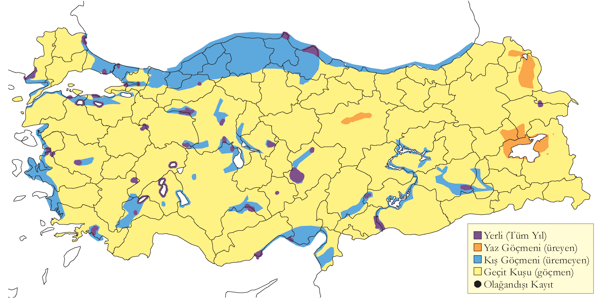
\includegraphics{images/harita_Page_023.png}

\hypertarget{uxfcreme-22}{%
\subsection{\texorpdfstring{\textbf{Üreme}}{Üreme}}\label{uxfcreme-22}}

\textbf{Yuvalama alanı}: Sazlıkların olduğu göllerde ve su aynalarının
bulunduğu geniş sazlıklarda ürer.\\
\textbf{Yuvası}: 19 Haziran 1984'te Erçek Gölü yakınlarındaki küçük bir
gölde sık bir örtü içindeki sazların dibine tutturulmuş sakarmeke
yuvasına benzer şekilde sudan yükseğe yapılmış bir yuva bulunmuştur; ölü
saz gövdeleri ve diğer bitkisel malzemelerin derin, düzgün bir kâse
şeklinde iç içe örülmesi ile oluşmuş dayanıklı bir yapı olan yuva bol
miktarda hav tüyü ve biraz da diğer tüylerle kaplanmıştır. Diğer
yerlerde, yuvalar genellikle benzer alanlardadır, nadiren su kıyısındaki
yoğun bitki örtüsünün içinde kuru zeminde de olabilir.\\
\textbf{Yumurta sayısı}: Türkiye'de yumurta sayısı kaydedilmemiştir,
gözlenen yavru sayısından 8-11 yumurta koyabileceği düşünülür. Diğer
yerlerde genellikle 6-9 yumurtadır. Gözlenen yavru sayısı ortalama
6,6'dır.\\
\textbf{Üreme dönemi}: Nisan başı ile haziran ortasına kadar yumurta
koyar. Yavrular temmuzda gözlenebilir. \textbf{KAR.} Kızılırmak
Deltası'nda, 11 Mayıs 1992'de hav tüyleriyle gözlenen birkaç günlük
yavru en erken kayıt\textsuperscript{44} yumurtlamanın nisanın ilk
haftasında olduğunu gösterir. 14 Haziran 1984'te yaklaşık 5 günlük bir
yavrulardan oluşan bir kuluçka ve yaklaşık üç haftalık yavrulardan
oluşan iki kuluçka gözlenmiştir\textsuperscript{24}. \textbf{İÇA.}
Haziran başlarında iki yumurtalı (tamamlanmamış) bir yuva bulunmuş ve
Haziran 1971 başlarında boz ördek yuvalarına iki, dört ve beş yumurta
bıraktığı tespit edilmiştir; 13 Mayıs 1991'de Hotamış'ta yumurtalı bir
yuva bulunmuştur\textsuperscript{48}. 1970 Mayıs sonlarında Eşmekaya'da
küçük yavrulardan oluşan beş yavru, 1 Haziran 1969'da Sultansazlığı'nda
altı yavru ve haziran-temmuzda diğer alanlarda da yavrular gözlenmiştir.
\textbf{DOA.} 19 Haziran 1983'te Van Sazlığı'nda yavrularıyla birlikte
sekiz dişi kaydedilmiştir.

\textbf{Alttürler ve Sınıflandırma}

Monotipik bir türdür.

\hypertarget{pasbaux15f-patka}{%
\section{Pasbaş Patka}\label{pasbaux15f-patka}}

Aythya nyroca

Ferruginous Duck

\textbf{Lokal olarak az sayıda üreyen yaz konuğu, yaygın ve nispeten çok
sayıda bulunan geçit türü, yaygın ancak az sayıda kış konuğudur.}

Tüm bölgelerdeki sulakalanlarda oldukça lokal bir yaz konuğudur. En
yüksek sayılarda İç ve Doğu Anadolu bölgelerinde bulunur. Kızılırmak
Deltası (1992'de tahminen 150-200 çift\textsuperscript{44}), Kocaçay
Deltası (1993'te tahminen 70 çift\textsuperscript{45}), Uluabat Gölü
(1988'de tahminen 32 çift\textsuperscript{53}) ve Göksu Deltası
(yaklaşık 30 çift) önemli sayılarda ürediği alanlardır. Son yıllarda
gerçekleştirilen çalışmalarda Güneydoğu Anadolu'da üç yeni üreme alanı
belirlenmiştir. Yaz göçmenleri mart ortasından eylül sonuna kadar
gözlenir.

Türkiye popülasyonu muhtemelen dünyadaki en önemlilerinden biridir ve
1000 ile 3000 çift arasında olduğunu düşünülmüş\textsuperscript{41},
sonra bu tahmin 500-600 çift olarak güncellenmiştir\textsuperscript{54}.
Avrupa'da yayılış alanının bir kısmında yaşanan sert düşüş dikkate
alındığında, Türkiye popülasyonun izlenmesine acil ihtiyaç
duyulmaktadır. 1990'ların sonlarında İç Anadolu'daki birkaç alanda da
azalma görülmüştür.

Geçiş sırasında az ve orta sayılarda bulunur ve ülke genelinde biraz
daha yaygındır. Az sayıda kışlar, 1992 yılında 105 birey, diğer yıllarda
50 bireyden az sayılmıştır. 1990'ların ortalarından itibaren kış
kayıtlarında bir artış gözlenmiş, bu durum muhtemelen gözlemci sayısının
artmasına bağlanmıştır. Eskiden batı ve orta bölgelerde daha çok sayıda
kışlamış, 1968-74 yıllarında 50 ile 450 birey arasında kaydedilmiştir.
Marmara Gölü'nde kaydedilen 860 birey en yüksek kayıttır. Doğu ve
Güneydoğu Anadolu'daki 2005 yılında sayılan 44 birey bahsedilmeye
değerdir.

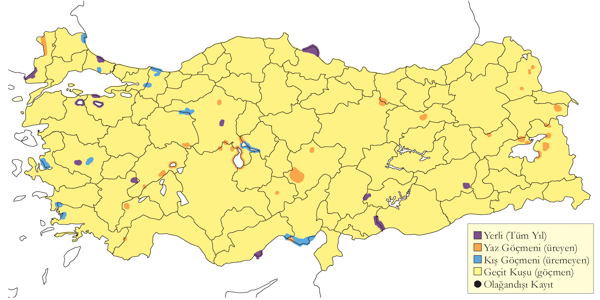
\includegraphics{images/harita_Page_024.png}

\hypertarget{uxfcreme-23}{%
\subsection{\texorpdfstring{\textbf{Üreme}}{Üreme}}\label{uxfcreme-23}}

\textbf{Yuvalama alanı}: Çevresinde sazlıkların ve yoğun su üstü
vejetasyonunun ve çoğunlukla daha geniş sazlıkların ve bataklığın
bulunduğu tatlı su göllerinde ürer.\\
\textbf{Yuvası}: Su kenarındaki yoğun vejetasyonun içine yuva yapar:
Kulu Gölü'ndeki bir adada, alçak çalıların arasında çıplak zeminde hafif
bir çukurun içine yapılan yuvanın ot ve hav tüyleriyle kaplandığı
gözlenmiştir (\textsuperscript{55}; A. Limbrunner, kişisel görüşme).\\
\textbf{Yumurta sayısı}: Türkiye'de gözlenen yumurta sayısı 6-8
arasındadır.\\
\textbf{Üreme dönemi}: Nisan ile Haziran başı arasında yumurta koyar.
Yavrular ağustosa kadar gözlenebilir. \textbf{MAR.} 19 Haziran 1999'da
Uluabat Gölü'nde bazıları küçük yavrulardan oluşan birkaç yavru grubu
gözlenmiş, 1966'da Manyas Gölü'nde yavru kaydedilmiştir. \textbf{KAR.}
Kızılırmak Deltası'nda çiftlerin çoğu sazlık alanlarda gözlenmiştir; 5
Mayıs 1992'de altı yumurtalı bir yuva bulunmuş ve 1 Haziran 1992'de
yumurtlamanın nisan sonlarından daha geç olmadığını gösteren üç ve dört
yavrulu iki grup\textsuperscript{44} kaydedilmiştir. 6 Ağustos 1971'de
yedi yavrulu bir grup gözlenmiştir. \textbf{AKD.} 15 Mayıs 1962'de
Çukurova'da sekiz yumurtalı bir yuva\textsuperscript{54}; 8 Mayıs
1953'te Amik Gölü'nde yumurtalı bir yuva\textsuperscript{54}; ve 27
Mayıs 1933'te yumurta kanalında yumurta bulunan bir dişi
vurulmuştur\textsuperscript{56}; Göksu Deltası'nda en erken 17
Haziran'da olmak üzere yedi savunma alanında yavrular gözlenmiştir.
\textbf{İÇA.} 28 Nisan 1982'de Sultansazlığı'nda yumurtalı bir yuva
bulunmuştur\textsuperscript{54}, Mayıs 1973'te Kulu Gölü'nde altı
yumurtalı bir yuva bulunmuştur; en erken 20 Haziran'da Eber Gölü'nde
olmak üzere Çöl Gölü, Gönenç Gölü, Sultansazlığı, Mogan Gölü ve Kulu
Gölü'nde yavrular gözlenmiştir. \textbf{DOA.} Yumurtlamanın mayıs
sonunda olduğunu gösterecek şekilde 1985 ve 1987 Haziran sonunda Van
Gölü'nde ve 29 Haziran 1987'de Edremit Sazlığı'nda yavrular
gözlenmiştir\textsuperscript{54}.

\textbf{Alttürler ve Sınıflandırma}

Monotipik bir türdür.

\hypertarget{tepeli-patka}{%
\section{Tepeli Patka}\label{tepeli-patka}}

\emph{Aythya fuligula}, Tufted Duck

\textbf{\emph{Lokal ve az sayıda üreyen yaz konuğu, nispeten yaygın ve
çok sayıda bulunan kış konuğudur.}}

Çok nadir ve lokal olarak üremiştir. Kızılırmak Deltası'nda, 1967 ve
1981'de Çalı Gölü'nde (Kars) ürediği kanıtlanmış ve son alanda 20
çiftlik bir popülasyon tespit edilmiştir. Başka bölgelerde düzenli
olarak yazı geçirir. Uluabat Gölü ve Uyuz Gölü gibi bazı alanlardaki
uygun habitatlarda çiftler gözlenmiştir. Üreme sonrasında Temmuz 1982'de
Kulu Gölü'nde tüy değişimi için toplandıkları düşünülen 700
birey\textsuperscript{43}, Eylül 1967'de Sodalı Gölü'nde çoğu erkek olan
1200 birey sayılmıştır.

Ülkenin batı ve orta bölgelerinde eylül başından nisanın başına kadar
kaydedilen yaygın ve bol olan bir geçiş türü ve kış konuğudur.
Karadeniz'de denizde kışlar. Kış ortası sayımlarında; 1968-69 kışında
20.800 birey, 1996 yılında en yüksek sayı olan 58.271 birey, 1992'de
yaklaşık 13.000 birey, 1993'te 16.965 birey (sadece Eğirdir Gölü'nde
10.478 birey) ve 1999'da 18.512 birey kaydedilmiştir. Son yıllarda ise
ülke toplamı genellikle 5000-10.000 birey arasındadır. En önemli kışlama
alanı Sapanca Gölü ve Eğirdir Gölü'dür.

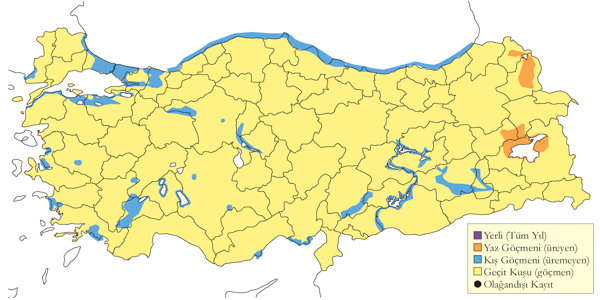
\includegraphics{images/harita_Page_025.png}

\hypertarget{uxfcreme-24}{%
\subsection{\texorpdfstring{\textbf{Üreme}}{Üreme}}\label{uxfcreme-24}}

\textbf{Yuvalama alanı}: Su üstü vejetasyonuna sahip olan tatlı su
göllerinde ürer.\\
\textbf{Yuvası}: Yuvasını bir bitki öbeğinin altına kurar.\\
\textbf{Yumurta sayısı}: Türkiye'de 8 yumurtalı bir yuva bulunmuştur.\\
\textbf{Üreme dönemi}: Mayıs ayında yumurta koyar, temmuz sonuna kadar
yavrular görülebilir. \textbf{KAR.} Kızılırmak Deltası'nda, 5 Mayıs
1992'de sazlıkta bir \emph{Juncus acutus} öbeğinin dibinde sekiz
yumurtalı bir yuva bulunmuş\textsuperscript{44} ve 28 Mayıs 1968'de de
ürediği kanıtlanmıştır\textsuperscript{24}. \textbf{DOA.} Çalı Gölü'nde
19 Temmuz 1992'de yavrularıyla birlikte iki dişi
gözlenmiştir\textsuperscript{57}.

\textbf{Alttürler ve Sınıflandırma}

Monotipik bir türdür.

\hypertarget{karabaux15f-patka}{%
\section{Karabaş Patka}\label{karabaux15f-patka}}

\emph{Aythya marila}, Greater Scaup

\textbf{\emph{Az sayıda ve düzenli olarak görülen kış konuğudur.}}

Karadeniz ve Marmara Bölgesi'nde hemen hemen her yıl az sayılarda
görülmektedir. Modern kuş tayinin başlaması sonrasında gelen kayıtlar
şöyledir\textsuperscript{1--4}: Ocak-Şubat 1969'da Sakarya Deltası'nda
yedi birey, Manyas ya da Uluabat Gölü'nde dört birey görülmüştür.
Kızılırmak Deltası'ndaki Liman Gölü'nde 1990'ların başlarında kışlayan
38 birey, 1970'lerde aynı alandan bildirilen şüpheli
kayıtların\textsuperscript{24}geçerli olabileceğini düşündürür.

Çoğu İstanbul civarından olan geçmiş veriler şöyledir: Şubat 1893'te,
Çekmece'de daha çok dişi ve gençlerden oluşan bir grup gözlemiş ve şu
anda Sofya Doğa Tarihi Müzesi'nde bulunan erkek örnek
toplanmıştır\textsuperscript{58}. İstanbul Robert Kolej'de bulunan dişi
örnek\textsuperscript{21}, 1998'deki bir ziyarette
bulunamamıştır\textsuperscript{59}. 1946-47 ve 1947-48 kışlarında
Çatalağzı açıklarında (Zonguldak) belirsiz sayıda
gözlenmiş\textsuperscript{60}, 15 Ocak 1950'de bilinmeyen bir yerden
altı örnek alınmıştır\textsuperscript{18}. Büyükçekmece'de Ocak 1963'te
bir erkek ve Şubat 1964'te bir dişi kaydedilmiştir\textsuperscript{18}.

Türün ilk yaz kaydı 30 Mayıs 1992'de Sodalı Gölü'nde kaydedilen iki
erkektir\textsuperscript{9}. Öte yandan, 19 Nisan 1981'de Kulu Gölü'nde
gözlenen iki birey, 12 Nisan 1990'da Göksu Deltası'nda gözlenen yaklaşık
20 birey\textsuperscript{10} olağandışı geç kayıtlardır.

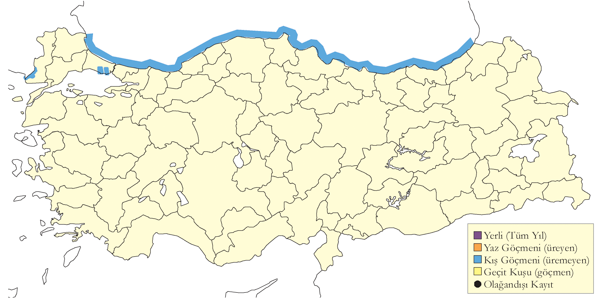
\includegraphics{images/harita_Page_026.png}

\hypertarget{uxfcreme-25}{%
\subsection{\texorpdfstring{\textbf{Üreme}}{Üreme}}\label{uxfcreme-25}}

Türkiye'de yuvalamaz. Avrasya ve Kuzey Amerika'nın kuzeyinde yuvalar.

\textbf{Alttürler ve Sınıflandırma}

Türkiye'de nominat alttürü bulunur.

\hypertarget{pufla}{%
\section{Pufla}\label{pufla}}

\emph{Somateria mollissima}, Common Eider

\textbf{\emph{Lokal ve az sayıda yerlidir. Türkiye'de üremez, en yakın
üreme kolonisi Ukrayna kıyılarındadır.}}

İlk üç kayıt şu şekildedir: 20 Eylül 1983'te Çernek Gölü'nde (Kızılırmak
Deltası) bir erkek\textsuperscript{24}, 3 Ocak 1984'te Göksu Deltası'nda
ölü bir dişi\textsuperscript{61}, 1 Şubat 1997'de, Sakarya Nehri
deltasının batısında Kefken açıklarında iyi tanımlanmış ilk kışında bir
erkek ve iki dişi\textsuperscript{62}bulunmuştur. Bundan sonra Riva,
Terkos Gölü kıyıları, İğneada, Kızılırmak Deltası, İzmit Körfezi ve
Sakarya Karasu'da 20'den fazla kayıtta 1-3 birey tespit edilmiştir.

Şubat 1929'un ilk yarısında Tarabya ile Beykoz arasında (İstanbul
Boğazı) gözlenen bir erişkin erkek\textsuperscript{18} tanım olmadığı
için burada kabul edilmemiştir. Güvenilir kayıtların tümü 1975 yılında
Ukrayna'nın Karadeniz kıyısında bir üreme alanının keşfedilmesinden
sonra olmuştur. Bu popülasyon 1990'ların ortasına kadar 1000 çifte
ulaşmıştır ve günümüze kadar artmaya devam etmektedir.

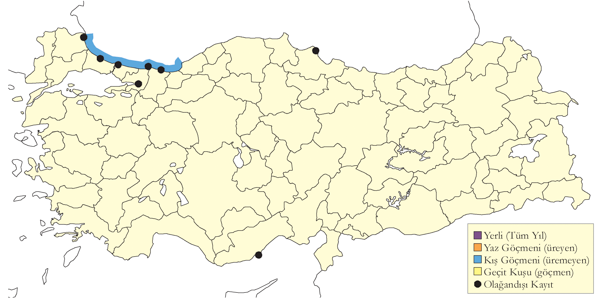
\includegraphics{images/harita_Page_027.png}

\hypertarget{uxfcreme-26}{%
\subsection{\texorpdfstring{\textbf{Üreme}}{Üreme}}\label{uxfcreme-26}}

Türkiye'de yuvalamaz. Ukrayna'daki koloni insan eli ile geliştirilmiş ve
bugün doğallaşmıştır. Doğal yuvalama alanı Kuzey Atlantik, Kuzey Buz
Denizi ve Bering Boğazı'dır.

\textbf{Alttürler ve Sınıflandırma}

Ülkede gözlenen ırk nominat \emph{mollissima} (Kuzeybatı Avrupa)
alttürüdür.

\hypertarget{kadife-uxf6rdek}{%
\section{Kadife Ördek}\label{kadife-uxf6rdek}}

\emph{Melanitta fusca}, Velvet Scoter

\textbf{\emph{Türkiye'de üreyen nüfus yok olmuştur, Gürcistan'da
yuvalamaya devam eden bireyler, Karadeniz kıyılarına az sayıda kışlar.}}

Doğu Anadolu'da az sayılarda kaydedilen çok lokal bir yaz konuğu idi. Az
sayıda yüksek irtifa göllerinde 3000 m'nin üstünde üremiş olduğu
düşünülür. Aktaş Gölü (Ardahan) kesin olarak ürediği tek alandır. 3 Ekim
1980'de 100 birey\textsuperscript{63} ve 14-15 Temmuz 1994'te aralarında
gençlerin de bulunduğu 725 birey\textsuperscript{64} kaydedilmiştir.

Geçmişte Nemrut Dağı'ndaki (Tatvan) krater Gölü'nde 20 çifte ürediği
düşünülmüştür. Ağrı Balık Gölü geçmişte ürediği sanılmış, ancak görünüşe
göre Haziran 2001'de (artık) üremediğine karar kılınmıştır. Çıldır
Gölü'nde ürediği güçlü şekilde şüphelenilmiş, ancak teyit edilmemiştir.
Kars Aygır Gölü ve Muş Nazik Gölü'nde azami 32 birey yazı geçirmiştir.
Doğu Karadeniz kıyılarında kışlayan bireylerin yaz aylarında da kaldığı
gözlenmiştir.

Orta ve Doğu Karadeniz boyunca az sayıda kışlar. 1995 Aralık sonunda
Yeşilırmak Deltası'nda 870 birey en yüksek kayıttır. Nadir olarak Batı
Karadeniz, Marmara'da ve güneyde Akdeniz kıyısında kışlamıştır. Ocak
1970'de Burdur Gölü'nde 27 birey, Şubat 1966'da Mogan Gölü'nde ve Ocak
2005'te Hazar Gölü'nde kaydedilmiştir. Son yıllarda kaydedilen 50 birey

4 Şubat 1917'de İstanbul Zeytinburnu açıklarında gözlenen iki birey ülke
için ilk kayıttır.

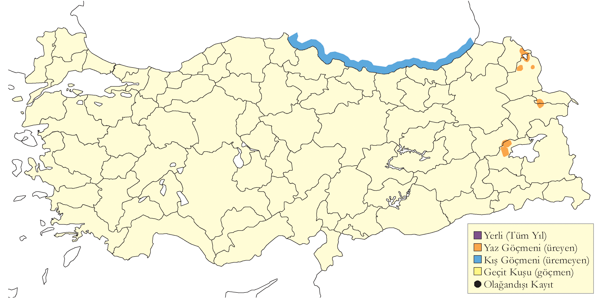
\includegraphics{images/harita_Page_028.png}

\hypertarget{uxfcreme-27}{%
\subsection{\texorpdfstring{\textbf{Üreme}}{Üreme}}\label{uxfcreme-27}}

\textbf{Yuvalama alanı}: Doğu Anadolu'daki iki ya da üç yüksek irtifa
gölünde üremiştir. Tüm çabalara rağmen Türkiye'de yuvası bulunamamıştır.
Şu anda Kafkasya popülasyonu sadece Gürcistan'da bir gölde
yuvalamaktadır.\\
\textbf{Yuvası}: Türkiye'de yuva bulunmamıştır ancak diğer yerlerde
yoğun bitki örtüsünün içine gizlenmiş şekilde yerde ve genellikle
göllerdeki adalarda yuva yapar.\\
\textbf{Yumurta sayısı}: Olağan yumurta sayısı 7-10'dur.\\
\textbf{Üreme dönemi}: Eski gözlemlere göre temmuz ve ağustos ayında
yuvalamıştır. \textbf{DOA.} 10 Temmuz 1967'de Nemrut Dağı'ndaki krater
Gölü'nde iki, yedi ve dokuz hav tüylü küçük yavru birlikte üç dişi ve 20
Ağustos 1967'de Balık Gölü'nde dört, beş ve altı yavrulu üç dişi
kaydedilmiştir\textsuperscript{52}. Küçük ördeklerin sadece yaklaşık bir
haftalık olduğu varsayılırsa yumurtlamanın haziranın ilk günlerinde
olduğu anlaşılmaktadır. 23 Ağustos 1972'de Nemrut Dağı'nda gözlenen
hemen hemen yarı gelişmiş yedi yavrulu bir dişi yumurtlamanın haziranın
son haftası olduğunu göstermektedir. 9 Temmuz 1985'te Nemrut Dağı'nda
beş çift ve iki genç birey gözlenmiştir. Son zamanlara ait bir üreme
kaydı yoktur ve 9 Haziran 2001'de Balık Gölü'ndeki adada yapılan
kapsamlı araştırmada ne yuva bulunmuş ne de erişkin görülmüştür.

\textbf{Alttürler ve Sınıflandırma}

Monotipik bir türdür. Eskiden Amerika ve Doğu Sibirya'da yaşayan
\textbf{Ak Kanatlı Kadife Ördek} \emph{Melanitta deglandi} ile aynı tür
olarak kabul ediliyordu.

\hypertarget{kara-uxf6rdek}{%
\section{Kara Ördek}\label{kara-uxf6rdek}}

\emph{Melanitta nigra,} Common Scoter

\textbf{\emph{Nadir kış konuğudur.}}

Karadeniz'de çoğunlukla eylül ve mart arasında çok az sayıda kaydedilen
kış göçmenidir. Düzenli olarak sadece Kızılırmak ve Yeşilırmak
Deltalarının açıklarında 20 birey kışlamaktadır. Karadeniz kıyısında
toplam 20'den fazla kaydı vardır. Marmara ve Ege'de çok nadirdir,
Akdeniz'de sadece bir kere kaydedilmiştir.

9 Nisan 1967'de Kocaçay Deltası'nda kaydedilen bir birey ülke için kabul
edilebilir ilk kayıttır\textsuperscript{1}. Öncesinde Ege'de nadir bir
kış göçmeni olduğunundan\textsuperscript{65} ve İstanbul Boğazı ve
Ceyhan Deltası'ndaki şüpheli kayıtlardan\textsuperscript{28}
bahsedilmiştir.

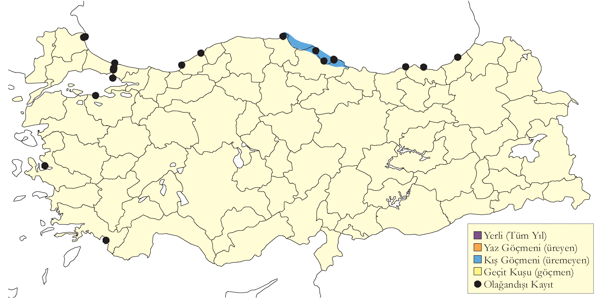
\includegraphics{images/harita_Page_029.png}

\hypertarget{uxfcreme-28}{%
\subsection{\texorpdfstring{\textbf{Üreme}}{Üreme}}\label{uxfcreme-28}}

Türkiye'de yuvalamaz. Avrasya'nın kuzeyinde yuvalar.

\textbf{Alttürler ve Sınıflandırma}

Monotipik bir türdür.

\hypertarget{telkuyruk}{%
\section{Telkuyruk}\label{telkuyruk}}

\emph{Clangula hyemalis}, Long-tailed Duck

\textbf{\emph{Nadir kış konuğudur.}}

Şubat 1893'te İstanbul (Büyük?) Çekmece'de, Alléon tarafından toplanan
genç bir dişi ülke için ilk kayıttır ve bu örnek Sofya Doğa Tarihi
Müzesi'nde görülebilir. Ardından, 13 Kasım 1968'de İzmit'te genç bir
birey kaydedilmiştir\textsuperscript{3}. Göksu Deltası Paradeniz
Gölü'nde 1-2 Ocak 1986'da bir birey ve 5 Ocak 1989'da bir
dişi\textsuperscript{61} görülmüştür. Sakarya Nehri ağzında 18 Şubat
2004'te\textsuperscript{66}; 26 Şubat 2006'da Fırtına Nehri'nin ağzında
birer birey fotoğraflanmıştır. En güncel kayıtlara göre; 7-19 Ocak
2008'de İğneada'da erişkin bir dişi, 13 Şubat 2008'de Kıyıköy'de bir
erkek, 10 Aralık 2008'de İğneada'da bir birey (onüçüncü kaydı) ve 28
Mart 2009'da Enez'de bir birey (on dördüncü kaydı)
görülmüştür\textsuperscript{8}.

İstisnai olarak, Van Gölü'nden 1977 ile 1987 arasında mayıs ve haziran
aylarında yaz kayıtları mevcuttur. 10 Haziran 1977'de Gevaş'ın batısında
Horkum'da iki birey ve Tatvan'la Ahlat arasında üç
birey\textsuperscript{5}, 22 Mayıs 1985'te Van'ın güneybatısında bir
erkek\textsuperscript{11}, 9 Haziran 1987'de Van Sazlığı'nda bir erkek
ve 22 Haziran 1987'de Van'ın 10 km. güneyinde bir
birey\textsuperscript{9} kaydedilmiştir.

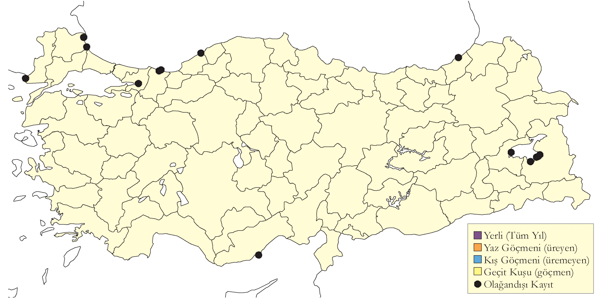
\includegraphics{images/harita_Page_030.png}

\hypertarget{uxfcreme-29}{%
\subsection{\texorpdfstring{\textbf{Üreme}}{Üreme}}\label{uxfcreme-29}}

Türkiye'de yuvalamaz. Kuzey İskandinavya dağlarında ve Rusya ve Kuzey
Amerika'nın tundra kuşağında yuvalar.

\textbf{Alttürler ve Sınıflandırma}

Monotipik bir türdür.

\hypertarget{altux131nguxf6z}{%
\section{Altıngöz}\label{altux131nguxf6z}}

\emph{Bucephala clangula,} Common Goldeneye

\textbf{\emph{Nispeten yaygın ve az sayıda kış konuğudur.}}

Karadeniz, Marmara ve Ege'nin kıyı bölgelerinde ve daha nadir olarak iç
bölgelerdeki sulakalanlarda ekim sonu ve nisan sonu arasında nadir bir
kış konuğudur. En düzenli olarak Marmara ve Karadeniz bölgelerinde
görülür. Kışın ülke çapında görülen kuş sayısı nadiren 100 bireyi geçer.
3 Şubat 1992'de Kızılırmak Deltası'nın açıklarında gözlenen 200 birey
kaydedilen en yüksek sayıdır. 2005-06 kışında Gediz Deltası'nda 72
birey, 3 Şubat 2002'de Gala Gölü'nde 60 birey
sayılmıştır\textsuperscript{67}. Son yıllarda ilkbahar sonunda Doğu
Karadeniz'de kaydedilmiştir.

1977 ile 1993 yılları arasında, Doğu Anadolu'da çoğunluğu Van Gölü'nde
bir dizi yaz kaydı vardır ve bunların bazılarında birden fazla birey
kaydedilmiştir. Bu kayıtlar yakınlarda üreyen bir popülasyonun
ihtimalini düşündürmüştür\textsuperscript{36}.

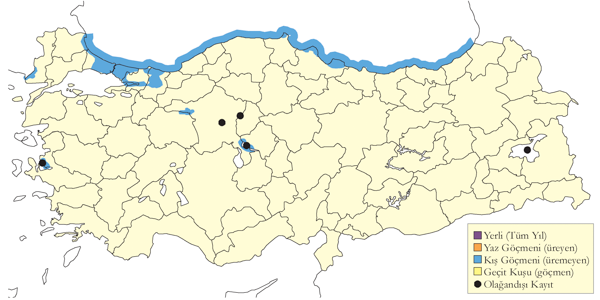
\includegraphics{images/harita_Page_031.png}

\hypertarget{uxfcreme-30}{%
\subsection{\texorpdfstring{\textbf{Üreme}}{Üreme}}\label{uxfcreme-30}}

Türkiye'de yuvalamaz. Avrasya ve Kuzey Amerika'nın kuzeyinde yuvalar.

\textbf{Alttürler ve Sınıflandırma}

Türkiye'de nominat alttürü bulunur.

\hypertarget{suxfctlabi}{%
\section{Sütlabi}\label{suxfctlabi}}

\emph{Mergellus albellus,} Smew

\textbf{\emph{Kuzey bölgelerine az sayıda gelen bir kış konuğudur.}}

Kasımdan nisan ortasına kadar ülkenin batı ve orta bölgelerindeki
sulakalanlarda ve kıyılarda tipik olarak nadir ve muhtemelen düzensiz
bir kış konuğudur. En çok Marmara'da, Karadeniz'de ve İç Anadolu'da
kaydedilir. Her kış genellikle 100 bireyden daha azdır. Uluabat Gölü'nde
1967'de 300, 1969-70'de 1300, 1973'te 555, 1989'da 111 ve 1995'de 248
birey kaydedilmiştir. 1992'de Manyas Gölü'nde 102 ve 1993'te
Büyükçekmece'de 79 birey kışlamıştır.

Nisan 1987 sonunda Diyarbakır'da kaydedilmiştir. Doğu ve Güneydoğu
Anadolu'da oluşturulan büyük baraj göllerinde gözlenmesi beklenebilir.
Ocak 1979'da Irak Razzaza Gölü'nde gözlenen 1000'den fazla
birey\textsuperscript{68} daha güneyde yüksek sayılarda
kaydedilebileceğini göstermektedir.

Ancak ne tuhaftır ki, türün ilk keşfi Strickland tarafından İzmir'den
alınan iki örnek ile yapılmıştır. Cambridge Üniversitesi Zooloji
Müzesi'ndeki koleksiyonda bulunan bu örnekler 6 Ocak 1836'da alınan bir
erkek ve aynı yıl şubat ayında alınan bir dişiye aittir. 1946-48
yıllarında Çatalağzı açıklarında (Zonguldak) oldukça bol olduğu
gözlenmiştir\textsuperscript{60}.

11 Haziran 1969'da Eymir Gölü'nde (Ankara) bir erkek\textsuperscript{2},
27 Haziran 1987'de Göründü'de (Van) bir dişi\textsuperscript{9} ve 27
Mayıs 1995'te Uluabat Gölü'nde bir erkek ve iki dişi\textsuperscript{10}
olmak üzere yazın üç defa kaydedilmiştir.

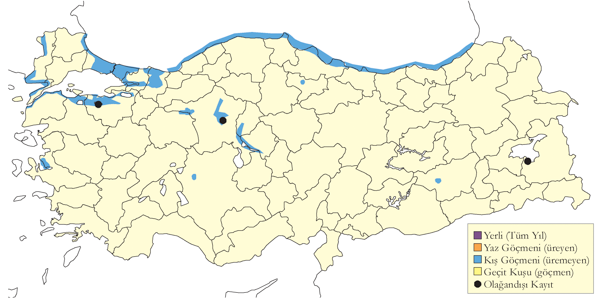
\includegraphics{images/harita_Page_032.png}

\hypertarget{uxfcreme-31}{%
\subsection{\texorpdfstring{\textbf{Üreme}}{Üreme}}\label{uxfcreme-31}}

Türkiye'de yuvalamaz. Avrasya'nın kuzeyinde yuvalar.

\textbf{Alttürler ve Sınıflandırma}

Monotipik bir türdür. Türkiye'de tanımlanmıştır.

\hypertarget{buxfcyuxfck-tarakdiux15f}{%
\section{Büyük Tarakdiş}\label{buxfcyuxfck-tarakdiux15f}}

\emph{Mergus merganser,} Common Merganser

\textbf{\emph{Nadir kış konuğudur.}}

Özellikle Marmara ve Karadeniz bölgelerinde az sayıda kaydedilen nadir
bir kış konuğudur. 1997-2007 arasında artan gözlemci aktivitesine karşın
sadece 10 kere kaydedilmiştir\textsuperscript{6}. Genellikle kıyısal
sulakalanlarda görülür, en düzenli olarak Kızılırmak ve Yeşilırmak
deltalarında kaydedilir. Kızılırmak Deltası'nda görüldüğü en geç tarih
20 Mayıs'tır.

Doğu Anadolu'da şubat ve martta iki defa, yazın üç kere gözlenmiştir; 11
Haziran 1970'de Pasinler ile Horasan arasında Aras Nehri üzerinde bir
çift, 7 Haziran 1986'da Van Gölü'nde bir birey ve 29 Haziran 1988'de
Bendimahi Delta'sında bir dişi ya da genç birey kaydedilmiştir.
Kurutulmadan önce Sevan Gölü (Ermenistan) havzasında üreyen bir tür
olduğu düşünülmüş, ancak ürediğine dair bir kanıt elde
edilmemiştir\textsuperscript{69}.

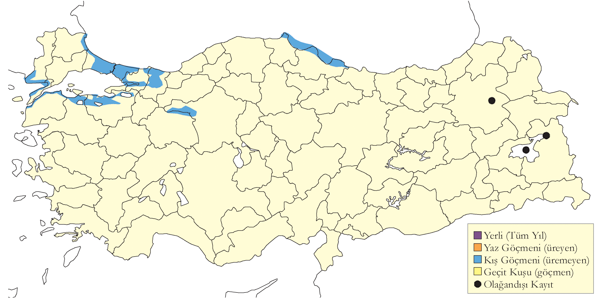
\includegraphics{images/harita_Page_033.png}

\hypertarget{uxfcreme-32}{%
\subsection{\texorpdfstring{\textbf{Üreme}}{Üreme}}\label{uxfcreme-32}}

Türkiye'de yuvalamaz. Avrasya ve Kuzey Amerika'nın kuzeyinde yuvalar.

\textbf{Alttürler ve Sınıflandırma}

Türkiye'de nominat alttürü bulunur.

\hypertarget{tarakdiux15f}{%
\section{Tarakdiş}\label{tarakdiux15f}}

\emph{Mergus serrator}, Red-breasted Merganser

\textbf{\emph{Nispeten lokal olarak ve orta sayılarda görülen bir kış
konuğudur.}}

Kıyısal alanlarda ekim sonu ve nisan sonu arasında kaydedilen kış
göçmenidir. En çok sayıda Doğu Karadeniz, Marmara ve Ege'de kaydedilir.
Gediz Deltası'nda düzenli olarak yaklaşık 100 birey konaklar, Şubat
1996'da 397 birey sayılmıştır. Büyük Menderes Deltası'nda Şubat 1993'te
67 birey ve Yumurtalık'ta 44 birey kaydedilmiştir. Ege ve Doğu
Akdeniz'deki alanlarda düzenli olarak önemi sayılarda
kışlar\textsuperscript{70}. Akdeniz kıyılarında seyrek olsa da Kıbrıs'ta
oldukça düzenli bir türdür.

20-21 Mayıs 1994'te Göksu Deltası'nda geç kalmış bir birey
kaydedilmiştir (Birdquest Newsletter 23: 59). Tek yaz kaydı 11 Haziran
1964'te Amik Gölü'nde (Antakya) kaydedilen yedi veya sekiz
bireydir\textsuperscript{71}.

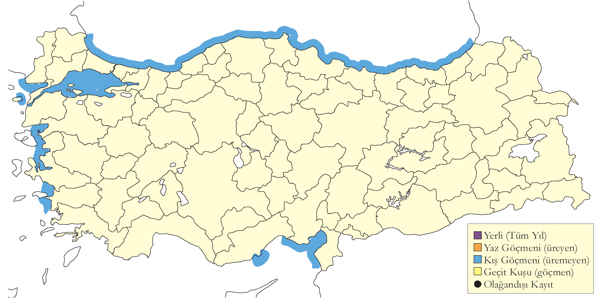
\includegraphics{images/harita_Page_034.png}

\hypertarget{uxfcreme-33}{%
\subsection{\texorpdfstring{\textbf{Üreme}}{Üreme}}\label{uxfcreme-33}}

Türkiye'de yuvalamaz. Avrasya ve Kuzey Amerika'nın kuzeyinde yuvalar.

\textbf{Alttürler ve Sınıflandırma}

Monotipik bir türdür.

\hypertarget{sec-dikkuyruk}{%
\section{Dikkuyruk}\label{sec-dikkuyruk}}

\emph{Oxyura leucocephala,} White-headed Duck

\textbf{\emph{Lokal olarak az sayıda üreyen yaz konuğu, nispeten yaygın
ve yüksek sayıda bulunabilen geçit türü ve kış konuğudur.}}

İç Anadolu ve Doğu Anadolu'da tatlı veya acı (sodalı), sığ ve ötrofik
göllerdeki yoğun sazlık sulakalanlarda az ila orta sayıda yuvalar. Van
Gölü çevresinde ve Kars'taki küçük sulakalanlarda ürediği teyit
edilmiştir. Doğu Anadolu'daki diğer alanlardaki üreme durumu
belirsizdir. Niğde Akkaya Barajı'nda üremiştir\textsuperscript{72}.
Üreme döneminde kaydedildiği Karadeniz Bölgesindeki bazı alanlarda
yuvalayabilir. Doğu Akdeniz sulakalanlarında yaz kayıtları üremeyen
bireylere aittir.

1980'lerin sonu ve 1990'ların başı arasında dört kilit alanda (Ereğli
Sazlığı, Hotamış Gölü, Sultansazlığı ve Kulu Gölü) üreyen İç Anadolu
popülasyonu muhtemelen 150 çiftin üzerindeydi. Ancak 1990'ların
ortasında Ereğli Sazlığı ve Hotamış Gölünün kurumasıyla sayıları
azalmış, Kulu Gölünde üremez olmuş\textsuperscript{73}. Kozanlı Gökgöl
ve Uyuz Gölü'nde az sayıda üremeye devam etmektedir.

Mart ile mayıs başı arasında birçok alanda geçiş sırasında gözlenir. 23
Mart 1992'de Kızılırmak Deltası'nda 1246 birey ve Mart 1990'da Ereğli
Sazlığı'nda 508 birey toplanmıştır. Mayıs ve haziran arasında toplanan
sürüler muhtemelen üreme alanlarına dağılacak kuşlardan oluşur. Temmuz
ve eylül arasında toplanan sürüler ise üreme sonrası dağılmaya ve göç
almaya işaret eder. Temmuzda Kulu Gölü'nde 500 birey ve ağustosta Sodalı
Gölü'nde 600-1000 birey kaydedilmiştir.

Kışın Akdeniz'deki birkaç sulakalanda yüksek sayıda, İç Anadolu'da
genellikle daha az sayıda kaydedilir. Batı ve orta bölgelerindeki diğer
yerlerde ise daha nadiren, özellikle sert hava koşullarında kaydedilir.
Karadeniz Bölgesi'nde düzensiz olarak yüksek sayılarda kışlar. Bir dönem
dünya popülasyonunun \%50'sinden fazlasının Burdur Gölü'nde kışladığı
düşünülmüştür; buradaki sayımlarda 1987'de 6400, 1988'de 9230, 1989'da
6700, 1991'de 10.927 birey\textsuperscript{74} kaydedilmiştir. Ancak
1992 sonrasında sayılarda azalma görülmüş; 1992'de 3264, 1993'de 3010 ve
1994'de 3337 birey sayılmıştır. Bu sayımlar son derece hassas olup, eş
zamanlı üç ekip tarafından ideal hava koşullarında gerçekleştirilmiştir.
Burdur Gölü'nde 1993'te 1991'e göre daha az genç bireyin sayılması, daha
düşük üreme başarısını gösterebilir. Bir ihtimal, Kazakistan ve çevre
ülkelerdeki üreyen nüfustaki azalış, Türkiye'deki kışlama nüfusunun
azalmasını açıklayabilir. Bu azalmada şüphesiz kaçak avcılığın da payı
vardır; 1992-93 kışında Burdur Gölü'nde muhtemelen 1000'den fazla
vurulmuştur. Ayrıca son yıllarda Burdur Gölü'nün kuruma sürecinin
başlaması ve tuzluluğun artması da bir etken olabilir.

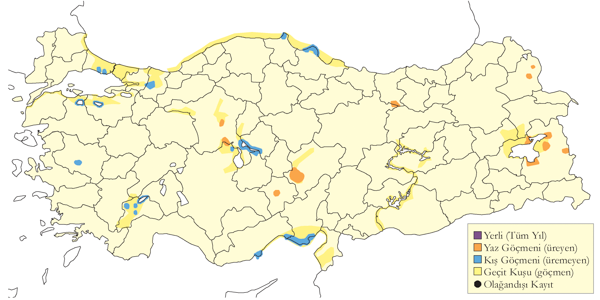
\includegraphics{images/harita_Page_035.png}

\hypertarget{uxfcreme-34}{%
\subsection{\texorpdfstring{\textbf{Üreme}}{Üreme}}\label{uxfcreme-34}}

\textbf{Yuvalama alanı}: Çoğunlukla büyük sulakalanların yakınlarında
genellikle 10 hektardan küçük ve 2 metreden sığ, sualtı vejetasyonu bol
ve su aynalarının bulunduğu geniş sazlıklara sahip olan tatlı su
göllerinde ya da sodalı göllerde ürer\textsuperscript{75}. Aynı alanda
birkaç çift üreyebilir.\\
\textbf{Yuvası}: Yuva, ölü saz gövdeleri ile diğer sucul bitkilerin
düzgün bir kâse oluşturacak şekilde örülmesi ile oluşturulmuş, birkaç
tutam açık gri tüyü ile astarlanmış dayanıklı bir yapıdır.\\
\textbf{Yumurta sayısı}: Bir yuvada en fazla 10 yumurta kaydedilmiştir.
19 Haziran 2004'te aynı gölde diz boyu derinliğindeki suda yoğun bir
sazlığın içinde iyice gizlenmiş bir şekilde suyun üzerinde dikey
sazların dibine tutturularak yapılmış bir yuvada on yumurtalı
tamamlanmış bir kuluçka bulunmuştur. Diğer yerlerde olağan yumurta
sayısı 5-12'dir. Dikkuyruk vücut ölçülerine göre son derece büyük ve
ağır yumurtalar koyar, yuva bu ağırlık nedeniyle suya batabilir.\\
\textbf{Üreme dönemi}: Mayıs başı ve temmuz başı arasında yumurta koyar.
Eylül sonuna kadar yavrular görülebilir. \textbf{İÇA.} 13 Temmuz
1987'de, Kulu Gölü'ndeki sazlıkların içindeki yuvada yedi yumurta
gözlenmiştir; muhtemelen dişinin kuluçkaya ara vermesi nedeniyle yuva ve
yumurtalar kısmen su altında kalmıştır\textsuperscript{75}. Üreme
kayıtlarının çoğu 3-10 yavrulardan oluşan gruplardır: İç Anadolu'daki en
erken kayıt 5 Haziran 1975'te Kulu Gölü'nde gözlenen üç büyük ve üç hav
tüylü yavru olup, yumurtlamanın mayıs başında olduğunu gösterir. 6
Ağustos 1972'de (kurutulmuş) Gönenç Gölü'nde 20 günlük beşer
yavrularıyla iki dişi ve dört günlük altı yavrulu bir dişi gözlenmiştir;
bu kayıtlar yumurtlamanın haziran ortası ile temmuz başında olduğunu
göstermektedir. İç Anadolu'da, temmuz ve ağustosta birçok yavrulu aile
kaydedilmiştir. \textbf{DOA.} Haziran-eylül ayları arasında Van Gölü'nde
9 Haziran 1987 ve 14 Haziran 1990'da gözlenen genç bireyler
yumurtlamanın mayıs ortasında olduğunu göstermektedir. Temmuz-ağustos
arasındaki diğer kayıtlar yumurtlamanın haziran ortasında başladığını
düşündürmektedir. Erçek Gölü yakınlarındaki küçük bir gölün ortasında
dikey sazlardan oluşan bir adada bir yuva bulunmuştur; sucul bitkiler
kullanılarak sazların dibine yapılmış olan yuvada 11 Haziran 2001'de iki
yumurta olduğu, kuluçkanın henüz tamamlanmadığı gözlenmiştir; alanda
sekiz erkek ve yedi dişi birey kaydedilmiştir ancak oldukça esaslı bir
araştırma yapılmasına rağmen başka bir yuva bulunmaması üremenin henüz
tam anlamıyla başlamadığını göstermektedir.

\textbf{Alttürler ve Sınıflandırma}

Monotipik bir türdür.

\bookmarksetup{startatroot}

\hypertarget{tavuksular}{%
\chapter{Tavuksular}\label{tavuksular}}

\hypertarget{orman-horozu}{%
\section{Orman Horozu}\label{orman-horozu}}

\emph{Lyrurus tetrix}, Black Grouse

\textbf{\emph{Türkiye'de soyu tükenmiştir. Eskiden lokal olarak az
sayıda bulunan yerli türdü.}}

Relikt bir popülasyonu 19. yüzyılın sonuna kadar İstanbul çevresinde
devam etmiş\textsuperscript{61}, ancak anlaşıldığı kadarıyla avlanma
sonucunda soyu tükenmiştir. İlk kez\textsuperscript{76},
sonrasında\textsuperscript{77} tarafından bahsedilmiştir. Son olarak
İstanbul Alemdağ çevresinde bulunduğu düşünülmüş\textsuperscript{78} ve
şehirde satılan ve nereden geldiği bilinmeyen ölü erkek bireyler tespit
edilmiştir\textsuperscript{21}. Aynı dönemde Bulgaristan popülasyonun da
ciddi oranda azaldığını kaydedilmiş\textsuperscript{79}, bu muhtemelen
avcılığa bağlanmıştır. Tür burada da uzun süreden beri tükenmiş
durumdadır. Genel olarak türün küresel yayılış alanı kuzey ve batıya
doğru daralmıştır\textsuperscript{22,80,81} Yunanistan'da 1935 yılından
bu yana Selanik ve Rodop Dağları çevresinden dört kayıt vardır.

\hypertarget{uxfcreme-35}{%
\subsection{\texorpdfstring{\textbf{Üreme}}{Üreme}}\label{uxfcreme-35}}

Türkiye'de yuvalamaz.

\textbf{Alttürler ve Sınıflandırma}

Türkiye'de yaşamış popülasyon muhtemelen nominat tetrix alttürüne
aittir. Literatürde \emph{Tetrao} cinsi altında da sınıflandırılmıştır.

\hypertarget{daux11f-horozu}{%
\section{Dağ Horozu}\label{daux11f-horozu}}

\emph{Lyrurus mlokosiewiczi}, Caucasian Grouse

\textbf{\emph{Lokal olarak az sayıda bulunan yerli türdür.}}

Doğu Karadeniz Dağlarının kuzey yamaçlarında sıklıkla karşılaşılmıştır.
3000 metre üzerinden gelen kayıtlar\textsuperscript{82} doğrulama
gerektirmektedir; ancak, neredeyse yerleşim yerlerine yakın (muhtemelen
15 kilometreye kadar) ve sonbahar ve kış mevsimlerinde düşük
yüksekliklerde bir miktar ağaç sınırının altında ve muhtemelen özellikle
şiddetli soğuklarda daha da düşük yüksekliklerde bulunurlar. Yayılış
bodur ormangülü Rhododendron ile alpin çayır kuşağının altındaki huş
Betula içeren yamaçlar üzerine yoğunlaşmıştır\textsuperscript{83}.

Artvin'in güneydoğusundan Gürcistan sınırı üzerinde Posof'a kadar
Yalnızçam Dağları'nda dar bir alanda bulunurlar. Yerel halktan alınan
bilgiler ışığında Gümüşhane'nın batısında ve Giresun çevresinde ve
muhtemelen Bingöl'e kadar güneyde, Cilo Dağları'nda bulunması olasıdır.

Türün lokal olarak nadir ya da doğu Karadeniz kıyı şeridi boyunca yaygın
yerli olduğu gösterilene kadar, geçtiğimiz yıllar içerisindeki
kayıtlarda görülen aşırı düzeydeki yetersizlik ile özellikle 1980 öncesi
kayıtlardaki eksiklikler türün Türkiye'de çok az bilinmesine neden
olmuştur. G. Neuhäuser Eylül 1943 tarihinde yüksek olasılıkla Türkiye
için ilk kayıt olan bir çift huş tavuğunu Rize ve Erzurum arasındaki
dağlardan toplamıştır\textsuperscript{28}.

Türkiye popülasyonunun muhtemelen \%90'nın görüldüğü Kaçkar Dağları'nda,
özellikle Sivrikaya çevresinde, 1993 yılında geçekleştirilen gözlem
çalışmalarında kur yapma amacıyla bir araya toplanan (lek poligini) 134
erkek gözlenmiştir. O tarihlerde yapılan tümevarımla toplam popülasyonun
2000 bireyden fazla olduğu tahmin edilmiştir\textsuperscript{57}.
Türkiye popülasyon büyüklüğü son zamanlardaki çalışmalara göre 1508-2675
birey arasında ölçülmüş ve tür 45 coğrafi yerde
kaydedilmiştir\textsuperscript{84}. Bu coğrafi yerlerin 29 tanesi yakın
bir zaman dilimi içerisinde keşfedilmiştir. Bunlardan 4 tanesi nispeten
ayrık popülasyonlardır. Türün yayılış sınırlarını ve popülasyon
büyüklüğünü tam olarak belirlemek için bilgisayar modellemesi
kullanılmıştır\textsuperscript{85}. Ancak, modellemenin sonuçları
bilinen ve yayılış haritasında gösterilen alanını genişletilememiştir.
Bununla birlikte 4900 bireylik popülasyon tahmini önceki en iyimser
tahminlerden bile çok yüksek olmuştur.

Türkiye popülasyonu yaylaların tatil konutlarına dönüşmesi sonucunda
artan yol inşaatları nedeniyle yaşam alanlarının terkedilmesi ile
parçalanmasından etkilenmekte ve nesli tehlike altına girmektedir. daha
az ölçüde avlanma baskısından (özellikle sonbahar döneminde görülen bir
problem) ve Tür için bir tehdit kaynağı olarak listelenen aşırı otlatma
bugün kaydedeğer ölçekte değildir, ancak bu durumun izlenmesi
gereklidir. Türün popülasyonlarının dengede ya da azalmakta olup
olmadığını ortaya koymak için türün popülasyonu ve yayılışı ile ilgili
tarihsel bilgiler yetersiz düzeydedir; ancak, popülasyonların
azalmasından şüphelenir.

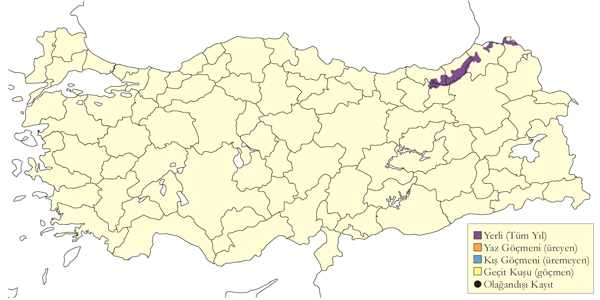
\includegraphics{images/harita_Page_037.png}

\hypertarget{uxfcreme-36}{%
\subsection{\texorpdfstring{\textbf{Üreme}}{Üreme}}\label{uxfcreme-36}}

Erkekler özellikle şafak ve gün batımında, eşeylerin çiftleşme amaçlı
karşılaştığı alanlarda biraraya gelerek bir arada kur gösterileri
(nümayiş) yaparlar. Türkiye'de sadece iki yuva türün en iyi bilindiği
lokalite, Sivrikaya'da (Rize) bulunmuştur. İlk yuva 2800-3000 metrede,
bodur Rhododendron çalılarının bulunduğu 3 hektarlık bir alanda
bulunmuştur. Yuva yoğun, kısa (1 metre) ve çok dallı çallılarda iyice
gizlenmiş olup, kökten çıkan dalların arasında, zeminde sığ bir çanak
şeklinde yapılmış, kuru dallar ve birkaç kuru Rhododendron yapraklarıyla
astarlanmıştır. Bu yuvada 6 Temmuz 1991 tarihinde 5 yumurta
kaydedilmiştir\textsuperscript{86}. Diğer kayıtlarda dişinin uçarak
uzaklaştığı bir yuvada 12 Temmuz 1993 tarihinde 4 yumurta görülmüş ve
bir yumurta kabuğu 11 Haziran 1997 tarihinde bulunmuştur. Bir erişkin
dişi ile tam gelişmemiş iki genç 12 Haziran 2003 tarihinde Ardahan,
Posof'da gözlenmiş ve yumurtlama zamanının mayıs başında başladığını
göstermiştir. Başka yerlerde, yaygın kuluçka küme büyüklüğü 5-6 (2-10)
adettir. Ermenistan'da, 30 Mayıs 1984'de bulunan bir yuva 8 yumurta
içermiş, bu yuvada ilk yumurtanın 21-23 Mayıs 1984 tarihinde bırakıldığı
belirlenmiştir. Bir diğer yuva 20 Mayıs 1985 tarihinde yumurta
içermektedir (ilk yumurta 13-16 Mayıs 1985 tarihinde bırakılmıştır) ve
bir diğeri 31 Temmuz 1994 tarihinde yumurta içermektedir. Bir dişi üç
genç bireyle (ergin büyüklüğünün \%25'ine ulaşmış) birlikte 5 Haziran
1980 tarihinde ve bir diğeri 26 Temmuz 1980 tarihinde tamamiyle büyümüş
5 genç içermektedir (Adamian ve Klem 1999). Ermenistan'dan üreme
döneminin daha erken gösteren kayıtlar Türkiye kayıtlarının normal üreme
dönemini yansıtıp yansıtmadığı hakkında bazı şüpheleri ortaya koymuştur.

\textbf{Alttürler ve Sınıflandırma}

Monotipik bir türdür. Rusca literatürde sıkça görüldüğü gibi, bazen
Lyrurus cinsi altında da sınıflandırılmıştır (farklı uygulamaların özeti
için bkz)\textsuperscript{87}.

\hypertarget{urkeklik}{%
\section{Urkeklik}\label{urkeklik}}

\emph{Tetraogallus caspius}, Caspian Snowcock

\textbf{\emph{Yüksek dağlarda lokal ve seyrek yerlidir.}}

Dağlık alanlarının yerlisidir. Üç önemli popülasyon Doğu Karadeniz
Bölgesi, Yüksekova ile Hakkari'ye ve İran sınırına kadar uzanan Doğu
Anadolu'nun dağlık kısımları ve yukarıda bahsedilen ve en batı sınırını
oluşturan Toroslar olarak belirtilebilir. En batıda Toros silsilesinde
Bolkar ve Melendiz dağlarında kaydedilmiştir. Yaz aylarında genellikle
2400 metrenin üzerinde kaydedilir. Ancak yazın Mersin'in kuzeyindeki
dağlarda 2000 metrenin altında görülmüştür. Ara sıra sonbahar döneminde
60 bireye kadar büyük gruplar oluşturular; bu grupların bazıları kış
ortasında alçak bölgelere inenler olabilir.

Eski kayıtlarda, en batıda Geyik Dağı, Alanya'nın kuzeyi ve Antalya'nın
dağlık alanlarında gözlenmiştir\textsuperscript{28}. Daha batıda
Akdağlar ve Beydağları'ndaki sürekli kar örtüsüne sahip zirveler uygun
yüksekliğe sahip alanlardır.

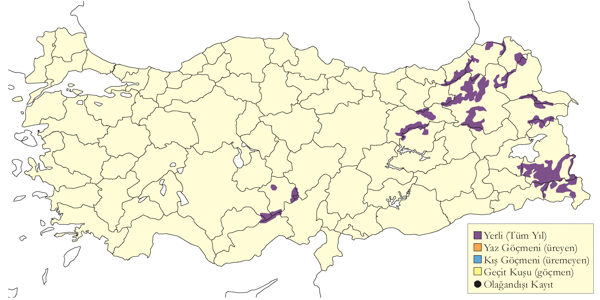
\includegraphics{images/harita_Page_038.png}

\hypertarget{uxfcreme-37}{%
\subsection{\texorpdfstring{\textbf{Üreme}}{Üreme}}\label{uxfcreme-37}}

Özellikle 2400 metre üzerinde, alpine çayırlarla kaplı, dik kayalıkların
ve yarların olduğu, yıl boyunca karlı ürerler. \textbf{KAR.}
Sivrikaya'da (Rize) beş genç ile bir ergin 12 Haziran 1989 tarihinde
küçük karlı alanları geçerken kaydedilmiştir.
\textbf{AKD.}\textsuperscript{88} Nisan 1876 tarihinde Toroslar
Aladağlar bölgesindeki yuvaları araştırmıştır. Karanfil Dağı'nda 2100
metre yükseklikte 23 Nisan 1876 tarihinde, bir dişi çıkıntılı bir kaya
ve ardıç kökü ile sarılmış bir yuvanın bulunduğu dik bir su yolundaki
küçük bir kaya üzerinden uçmuştur. Yuva taşlı toprak üzerinde derin
yuvarlak bir oyuk olup yetersiz düzeyde kuru otlar ve birkaç kuş tüyüyle
astarlıdır. Bu yuvada altı yumurta kaydedilmiştir. 25 Nisan 1876
tarihinde Bolkar Dağları'ndaki iki yuva benzer özelliklerde
kaydedilmiştir. Ancak bir tanesi yeşil köknar ibreleri ile
astarlanmıştır. Bu yuvalarda altı ve dört yumurta kaydedilmiştir.
Yukarıdaki üç yuvanın ikisinden alınmış iki yumurta Manchester
Müzesi'nde saklanmaktadır. Bu yuvaların ikisinden alınan altı yumurta,
Anadolu'dan 1 Haziran 1894 tarihinde toplanmış ekstra bir yumurta ile 5
Nisan 1901 tarihinde Aladağlar'dan muhtemelen tamamlanmamış bir
kuluçkadan toplanan üç yumurta Tring'deki Doğa Tarihi Müzesi'nde
saklanmaktadır. Son yıllarda, 8 Temmuz 1986 tarihinde Aladağlar'da, 1-2
haftalık 5 genç ile bir ergin gözlenmiş olup, ilk yumurta 21 Mayıs
tarihinde bırakılmış olmalıdır. Çil keklik büyüklüğünde 5-6 ferik ile
bir dişi 3-5 Ağustos 1967 tarihinde (Vielliard 1968) kaydedilmiştir. 19
Ağustos 2000 tarihinde, bazıları erginlerden belirgin derecede küçük 3-4
ferikli en azından üç aile grubu kaydedilmiştir. 6 Ağustos 1966
tarihinde Karanfil Dağı üzerinde 3000 metre yükseklikte iki ergin ve iki
genç kaydedilmişir\textsuperscript{89}.

Ermenistan'da ortalama yumurtlama dönemi 10-15 mayıs arasında, kuluçka
dönemi 20-30 mayıs arasında olup yuvalardan çıkan ferikler 13 Haziran
tarihinde kaydedilmiştir\textsuperscript{69}. Gençlere ait bazı erken
kayıtlar ilk yumurtanın 23 Nisan veya öncesinde bırakıldığını ortaya
koymaktadır. Nisan sonu ile mayıs başını içeren iki kayıt Danford'un
Türkiye'de kaydettiği yuva tarihleri ile kabaca uyum göstermektedir.

\textbf{Alttürler ve Sınıflandırma}

Monotipik bir türdür. Eskiden Hakkari ve Zagros Dağları'ndaki kuşların
\emph{semenowtianschanskii} (Zarudny, 1908), Toros Dağları'nda
\emph{tauricus} (Dresser, 1876) ve Erzurum bölgesinde \emph{challayei}
isimli ayrı alttürlerin olduğu düşünülmüştür.

\hypertarget{kux131nalux131-keklik}{%
\section{Kınalı Keklik}\label{kux131nalux131-keklik}}

\emph{Alectoris chukar}, Chukar Partridge

\textbf{\emph{Yaygın ve çok sayıda bulunan yerlidir.}}

Yaygın ve Trakya ile Batı Karadeniz kıyı şeridi içerisinde nadir,
Türkiye genelinde oldukça bol yerli bir kuş türüdür. İç bölgelerde
genellikle 700-2000 m arasında görülür. Genellikle kurak, kayalık tepe
ve dağlık alanlarda en az 2800 metreye kadar görülmüştür. Hemen hemen 40
bireye kadar çıkabilen ve gençleri de içeren oldukça büyük sürüler
kaydedilmiştir.

Geçmişte özellikle Hatay ve Doğu Karadeniz kıyı şeridi gibi bölgelerde
oldukça bol olarak kaydedilmiştir. Belirgin bir azalma göstermektedir.

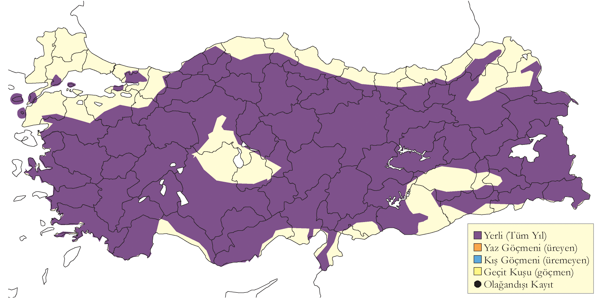
\includegraphics{images/harita_Page_039.png}

\hypertarget{uxfcreme-38}{%
\subsection{\texorpdfstring{\textbf{Üreme}}{Üreme}}\label{uxfcreme-38}}

Bodur çalılar ile kurumuş tarım alanlarının bulunduğu kayalık ve taşlık
tepelerle oldukça kurak ve çorak alanlarda ürer. Yerde yuvasını bir çalı
ya da bitki dibine gizler. \textbf{EGE.} Kuluçkadaki bir ergin birey
İzmir yakınlarında 14 yumurta içeren bir yuvadan\textsuperscript{90} 7
Mayıs 1951 tarihinde alınmıştır. Yuva yuvanın sahibi olan kuşun çok
sayıda tüyü ile birlikte çalı benzeri bitkilerle astarlanmış ve dikenli
meşe ile de korunmuştur. Yumurtalar krem ile kırmızı arasında bir
renklenme ile kırmızımsı küçük beneklenmeler gösterir
{[}@\textsuperscript{91}1950{]}. \textbf{AKD.} 11 Mayıs 1899 tarihinde
Acıgöl'de 5 yumurtalı bir yuva kaydedilmiştir, dişinin yumurtlamaya
devam edeceği düşünülmüştür\textsuperscript{30}. Karadağ'da, taze
yumurtalar içeren iki yuva 1907 yılının Mayıs sonunda kaydedilmiştir. Bu
yuvada taza yumurtlar haziran ayında da bulunmuştur . Bir ergin ile 5-6
iyi gelişmiş genç birey Burdur ve Bucak arasındaki geçitte 13 Temmuz
1968 tarihinde kaydedilmiştir\textsuperscript{92}. \textbf{İÇA.} 22
yumurta içeren bir yuva 24 Mayıs 1998 tarihinde Ereğli yakınlarındaki
bir kraterin, bir çalı ile sarılmış kaya çıkıntısı üzerinde
kaydedilmiştir. 20 yumurtadan 9 tanesi nisan ayı sonunda bırakılmıştır
(Banoğlu ve Burr 1953). \textbf{DOA.} Nemrut Dağı'nda (Bitlis), 9
Haziran 2004 tarihinde sabah saatlerinde 15 yumurtalı bir yuva
kaydedilmiştir. Ancak, günün ilerleyen saatlerinde, ergin bir birey yuva
üzerine oturmuştur. Muhtemelen bu tarih inkübasyonun ilk günü olarak
belirtilebilir. Yuva kısmen yaprak döken ormandaki bodur çalılar altında
bulunur. Zemine derin bir şekilde kazılmış ve birkaç adet ergin kuş tüyü
ve otların kökleri ile astarlanmıştır. \textbf{GDA.} Kuluçka kayıtları 2
Haziran 2001 tarihinde Işıklı'da (Gaziantep) gençleri içermektedir ve 22
Haziran 1966 tarihinde Menemen (İzmir) yakınlarında 6, 7 ve 8 yavrulu
içermektedir. Akdeniz Bölgesi'nde 22 Mayıs 1989 tarihinde bir kuluçka ve
30 Haziran 1966 Aladağlar'da birkaç günlük genç bir birey
kaydedilmiştir. Birkaç kuluçkanın birleşmesi sonucunda oluşan ve yaygın
olarak gözlemlenmeyen büyük kuluçkalar, tek bir ergin ile birlikte 13
Ağustos 1967 tarihinde Kızılcahamam'da (Ankara)
kaydedilmiştir\textsuperscript{93}.

\textbf{Alttürler ve Sınıflandırma}

Cypriotes alttürü Türkiye'nin güneyi boyunca görülmektedir. Kuzeyde
kleini ve Doğu Akdeniz bölgesine özgü sinaica alttürünün etki gösterdiği
bölgede, Güneydoğu Anadolu'da, kurdestanica alttürü bulunmaktadır. Tür
içerisinde coğrafi varyasyon konusu ile ilgili bir çıkarım yapamadık;
ancak, gözlemlenen formların tamamı güçlü bir şekilde gradient ile
birlikte belirgin klinal yapı göstermektedir\textsuperscript{81}.

\hypertarget{kum-kekliux11fi}{%
\section{Kum Kekliği}\label{kum-kekliux11fi}}

\emph{Ammoperdix griseogularis}, See-see Partridge

\textbf{\emph{Nispeten yaygın ve çok sayıda bulunan yerlidir.}}

Son zamanlara kadar çoğu Suriye sınırının 50 km içinde yer alan 15
coğrafi yerde biliniyordu ve 40 bireylik grupların kaydedildiği sonbahar
mevsimi dışında nadiren düşük sayılardan daha fazla kaydedilmişti.
Ancak, Türkiye'nin güneydoğusunda son zamanlarda yapılan gözlemler uygun
habitatların olduğu alanlar ile birlikte türün hemen hemen 50 coğrafi
yerde bulunduğunu göstermiştir\textsuperscript{94}.

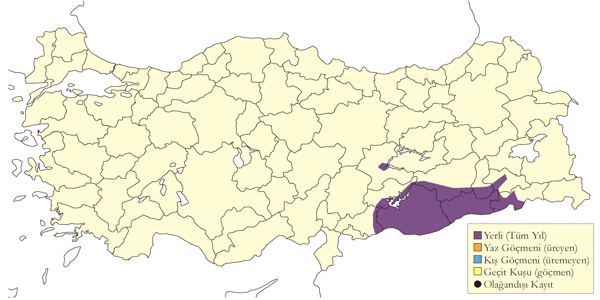
\includegraphics{images/harita_Page_040.png}

\hypertarget{uxfcreme-39}{%
\subsection{\texorpdfstring{\textbf{Üreme}}{Üreme}}\label{uxfcreme-39}}

Güneydoğu Anadolu'da zayıf vejetasyon örtüsüne sahip kurak kayalık
alanlarda üremektedir. Türkiye içerisinde yuva ve yumurta tanımlaması
yapılmamıştır; ancak, diğer yerlerde, yuvalar yuvanın bulunduğu yere
yakın bitki materyalleri ve otlarla astarlanmış, genellikle taş ya da
bir tutam bitki ile çevrelenmiş şekilde zeminde, toprağa kazılmış halde
bulunur. Kuluçka küme büyüklüğü genellikle 8-12 arasındadır, bazen
yumurta sayısı 16'ya kadar çıkabilmektedir. Nisan ayında çiftler
kaydedilmiştir. 5-7 Haziran 1973 tarihinde Halfeti'de kaydedilen üç
haftalık üç genç birey ile bir ergin, diğer yerlerde kaydedilen ilk
yumurtayı koyma tarihiyle çelişmeyecek şekilde ilk yumurtaların nisan
ortasında bırakıldığını göstermektedir. 2004-05 yıllarında Birecik'te
bir kaç tane genç birey kaydedilmiştir. 11 Ağustos 2001 tarihinde
Cizre'de bir aile kaydedilmiş, gençlerin boyu hakkında detaylar
verilmemiştir.

\textbf{Alttürler ve Sınıflandırma}

Monotipik bir türdür.

\hypertarget{turauxe7}{%
\section{Turaç}\label{turauxe7}}

\emph{Francolinus francolinus}, Black Francolin

\textbf{\emph{Lokal ve yer yer çok sayıda bulunan yerlidir.}}

Çukurova ve Göksu Deltaları ve çevresinde, ayrıca Suriye sınırında Fırat
ve Dicle nehirleri boyunca ürer. Çukurova'da çoğu Akyatan Gölü
yakınlarında bulunan (75 çift) ve toplam 85 çifte ulaşan üreme
popülasyonu kaydedilmiştir\textsuperscript{57}. Göksu Delta'sında, çoğu
kumullarda olmak üzere 50 üreme çifti
kaydedilmiştir\textsuperscript{57}. Güneydoğu Anadolu'da yaklaşık 15
lokaliteden kaydı vardır\textsuperscript{95}.

Yayılış sınırları doğu bölgelerdeki tarımsal faaliyetlerin artması
sonucu tür için oluşan uygun habitatların artması ile doğuda görünür bir
şekilde genişlemesine karşın, mevcut durumu ve ekolojisi
derlenmiştir\textsuperscript{96}. Doğu Akdeniz'deki bazı yerlerde tür
için koruma tedbirleri uygulanmıştır.

Eskiden Güneydoğu Marmara ile Ege Bölgesi'nin güney kıyılarının bazı
bölümlerinde yerli olarak kaydedilmiştir\textsuperscript{97}. Ancak, her
iki bölgede 19. yüzyıl içinde ortadan kalkmıştır. İstanbul Boğazı
çevresinden 1850'li yıllardan gelen tek bir kayıt vardır. Göller Bölgesi
ile Anti-Toroslara kadar kuzeyde, 600 metreye kadar oldukça lokal olarak
kaydedilmiştir\textsuperscript{28}. Ekim 2003 tarihinde Tavas, Denizli
çevresinden muhtemelen tutsak bir bireyin kaçması sonucu güncel bir
kayıt gelmiştir. Daha güncel kayıtlar türün 1960'lı yıllardan bu yana
türün Akdeniz Bölgesi'nin batısında Köyceğiz Gölü'nde kaydedilmediğini
ve ortadan kalktığını göstermektedir.

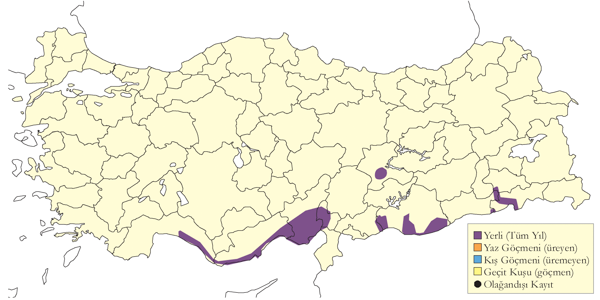
\includegraphics{images/harita_Page_041.png}

\hypertarget{uxfcreme-40}{%
\subsection{\texorpdfstring{\textbf{Üreme}}{Üreme}}\label{uxfcreme-40}}

Çalı ve çalı dışındaki bitki örtüsüne sahip kumullar ile ot, çalı ve
bodur bitkilerin arasındaki oyuklarda yaşarlar. Ayrıca, olgunlaşmamış
çalıların bulunduğu nemli (ıslak olmayan) alanlar, nehir kıyıları ve sık
ılgın (Tamarix) çalılarından oluşmuş sık topak şeklindeki çalılık
alanlarda ile mısır tarlalarında ürerler. Kum tepelerinde (her 2-5
hektarda bir erkek) ve tarım alanlarında (15-30 hektarda bir erkek)
yüksek yoğunluktadırlar (van den Berk 1988). \textbf{GDA.} Birecik'in
güneyinde Suriye sınırına yakın bölgelerdeki geniş mısır tarlarından
üredikleri kesin olan erginlerin sesleri duyulmaktadır. Benzer durum
Kıbrıs'ta da kaydedilmiştir. \textbf{AKD.} Göksu Deltası'ndaki kum
tepelerinde, 17 Haziran 1992 tarihinde muhtemelen bir önceki yıldan
kalmış bir yuva kaydedilmiştir. Yuvada güneşten etkilenmiş ve solgun
renklere sahip yumurta kabukları bulunmuştur. Yuva astarlanmamış, kum
içerisinde birkaç bitki parçasıyla çevrelenmiş sığ bir oyuk şeklinde ve
zemininde bir tutam ot içermektedir. Yumurtalar: Türkiye'den veri yok;
diğer yerlerde ise kuluçka küme büyüklüğü genellikle 8-12 (7-18)
arasındadır. Göksu'da, en azından 1-2 günlük 7 genç ile bir dişi 5 Mayıs
2004 tarihinde kaydedilmiştir. Bu kayıt ilk yumurtanın 9 Nisan'da
bırakıldığını göstermektedir. Bir ergin ile bir genç kuş 20 Temmuz 1986
tarihinde gözlenmiştir. Çukurova'da, yerel halk yavruları 10 Mayıs 1986
tarihinde yakalamıştır (yaygın oldukları bildirilmiştir). Bu tarih
yumurta bırakma zamanının yaklaşık nisan ortasında olduğunu
göstermektedir. Ötüşteki artış ise nisan ayının ikinci yarısı ile mayıs
ayının ilk yarısında tepe yapmaktadır (van den Berk 1988). Banoğlu ve
Burr (1953) tarafından yapılan bir diğer açıklamada ``dişi kuşlar mart
ayı sonu ile nisan ayı içerisinde yuvaları ve yumurtaları ile
meşguldürler'' ifadesine yer verilmiştir. Yumurtalar keklik (kınalı
keklik) yumurtaları büyüklüğünde ve açık yeşil renktedirler; Seyhan ve
Ceyhan kıyılarındaki (Çukurova) sık örtüşe sahip bodur ağaçlıklar
arasında zemine bırakılır. Dörtyol ve Alik civarında, dik ve derin
vadilerdeki kayalıkların sınırlarına ya da adalar arasındaki saz
yatakları araları ile bodur ağaçlıklar ve çalı topakları içine
yuvalanırlar. Eskiden Adana civarındaki düzlüklerde çok sayıda
görülürlermiş. Manchester Müzesi'ndeki üç yumurta (tamamlanmamış bir
kuluçkadan) İzmir yakılarından 10 Mayıs 1899 tarihinde alınmıştır. Tring
Doğa Tarihi Müzesi'ndeki dört yumurtanın ikisi Mersin'den 7 Mayıs 1884
tarihinde ve diğer ikisi 15 Mayıs 1899 tarihinde Anadolu'da bilinmeyen
bir lokaliteden alınmıştır.

\textbf{Alttürler ve Sınıflandırma}

Türkiye'de nominat alttürü bulunur. Meinertzhagen tarafından Amik Gölü
(Hatay) bölgesinden tanımlanmış \emph{billypayni} alttürü sinonim olarak
kabul edilmektedir.

\hypertarget{uxe7ilkeklik}{%
\section{Çilkeklik}\label{uxe7ilkeklik}}

\emph{Perdix perdix}, Grey Partridge

\textbf{\emph{Yaygın ancak seyrek yerlidir.}}

Tür özellikle ovalardaki tarım alanlarında, uzun boylu ot
topluluklarının kenarlarında ve 2250 metreye kadar birincil yarı step
alanlarda ürerler. Muhtemelen Trakya'da nesli tükenmiş ve Karadeniz kıyı
şeridinde oldukça lokaldir. Geçtiğimiz 20 yıl içerisinde tarımın
yoğunlaşması, aşırı otlatma ve avlanma nedeniyle popülasyonu önemli
derecede azalmıştır.

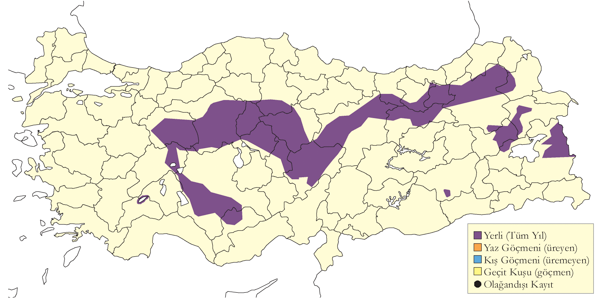
\includegraphics{images/harita_Page_042.png}

\hypertarget{uxfcreme-41}{%
\subsection{\texorpdfstring{\textbf{Üreme}}{Üreme}}\label{uxfcreme-41}}

Genellikle açık tarım alanlarında üremektedirler. Türkiye içerisinden
yuva tanımı yapılmamıştır, ancak diğer yerlerden gelen bilgilere göre
yuva ot ve ölü yapraklarla astarlanmış, genellikle vejetasyon içerisine
iyi bir şekilde gizlenmiş ve zeminde yer alan sığ oyuklar şeklindedir.
\textbf{İÇA.} 11 Haziran 1977 tarihinde bir genç ile bir ergin Mogan
Gölü'nde, 16 Temmuz 1977 tarihinde 8 genç Emir Gölü'nde ve 28 Ağustos
1984 tarihinde 7 bireylik bir aile Çavuşcu Gölü'nde kaydedilmiştir.
\textbf{GDA.} Diyarbakır yakınlarında, 16 Mayıs 1999 tarihinde gevenle
(\emph{Astralagus} sp.) örtülü bir yamaçta on yumurta içeren bir yuva 27
Mayıs'ta 19 yumurta içermiştir\textsuperscript{98}. Diğer yerlerdeki
yaygın kuluçka küme büyüklüğü 9-20 (23) arasındadır. Bazen iki dişinin
aynı kuluçkayı paylaşması nedeniyle büyük kuluçkalar da kaydedilebilir.

\textbf{Alttürler ve Sınıflandırma}

Trakya'da nominat \emph{perdix} alttürü, Anadolu'da \emph{canescens}
alttürü bulunmaktadır. Doğaya salınan değişik orijinden bireylerin yerel
kuşlarla karışması nedeniyle türün yayılış alanı içindeki coğrafi
varyasyonu oldukça karışıktır\textsuperscript{81}.

\hypertarget{bux131ldux131rcux131n}{%
\section{Bıldırcın}\label{bux131ldux131rcux131n}}

\emph{Coturnix coturnix}, Common Quail

\textbf{\emph{Yaygın ve çok sayıda bulunan yaz konuğu ve geçit türü,
nadir kış konuğudur.}}

Çoğunlukla tahıl ekilen kurak tarlalar ve bozkırlarda, çayırlar ve
yüksek otların bulunduğu dağlık bölgelerin yanında yoğun vejetasyonlu
kumullar gibi alanlarda bulunur. Özellikle İç Anadolu'da oldukça yaygın
olarak ürese de hububat tarımının nispeten az olduğu kıyısal bölgelerde
oldukça azdır. Doğu kesimlerinden en azından 2300 metreye kadar
üreyebilir. Üreme ve geçit sırasında özellikle tahıl ekilen arazilerde
bulunur.

Üreme dışında geçit sırasında tüm ülkede bol sayıda bulunur. İlkbahar
geçişi mart sonu ve nisan arasında, sonbahar geçişi ise ağustos sonu ve
eylül boyunca, hatta kuzey bölgelerinde daha da erken olur. Az sayıda
Ege ve Akdeniz kıyılarında kışlar, bu durum geçişin sonunun tespitini
zorlaştırır. Karadeniz kıyılarında da kasıma kadar göçünün sürdüğü
bilinir\textsuperscript{99}. En kuzey bölgelerinde mart sonundan
itibaren görülür. Kasım sonunda 26 Kasım 2003 Seyfe Gölü'nde ve 20 Kasım
2010'da Nallıhan Kuş Cenneti'nde görülmesi geç geçitle
ilgilidir\textsuperscript{100}. Çok az sayıda Batı ve Güney bölgelerinde
kışlayabilir.

Tarım arazilerinde yaşayan diğer kuşlar gibi tarımın yoğunlaşması, tahıl
dışındaki ürünlerin çoğalması ve avcılık sonucunda sayıları ülke çapında
azalmıştır. Göçmen kuşlar aşırı av baskısı altındadır ve özellikle
Karadeniz bölgesinde yasadışı yakalama devam etmektedir.

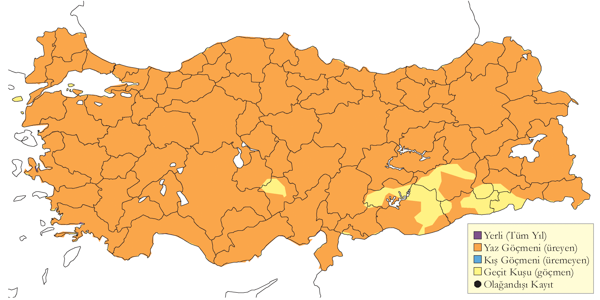
\includegraphics{images/harita_Page_043.png}

\hypertarget{uxfcreme-42}{%
\subsection{\texorpdfstring{\textbf{Üreme}}{Üreme}}\label{uxfcreme-42}}

\textbf{Yuvalama alanı}:\\
\textbf{Yuvası}:\\
\textbf{Yumurta sayısı}:\\
\textbf{Üreme dönemi}:

Ürediğini kanıtlamak son derece zordur ve Türkiye'de henüz bir yuvası
tespit edilmemiştir. Türkiye kışında; yerdeki düzce bir çukuru ot ve
yakındaki bitkisel materyal ile astarlar. Genellikle 7-12 arasında
istisnai olarak 6 18 arasında yumurta koyar. \textbf{MAR.} Uluabat
Gölü'nde 22 Mayıs 1966'da yavrular gözlenmiştir. Çoğu bölgeye ilkbaharda
Nisan ortasından gelir ve tüm yavru gözlemleri üremenin alana varıştan
hemen sonar başladığını gösterir. Ağustos'ta duyulan kuşlar gecikmiş bir
üremenin göstergesi olabilir. \textbf{GDA.} Birecik'te 4 Haziran 1993'de
tamamen palazlanmış 3 haftalık 9 yavru, hasat döneminde biçilmiş mısırın
altında saklanırken görülmüş ve köylüler tarafından yenmek üzere
yakalanmıştır. 5 Haziran 1993'de görülen başka 6 kuş yumurtlama
tarihinin yaklaşık 20 Nisan'da olduğunu gösterir. Suriye'de yavrularıyla
dolaşan bir çift Temmuz'da gözlenmiştir\textsuperscript{39}.

\textbf{Alttürler ve Sınıflandırma}

Türkiye'de nominat alttürü bulunur.

\hypertarget{suxfcluxfcn}{%
\section{Sülün}\label{suxfcluxfcn}}

\emph{Phasianus colchicus}, Common Pheasant

\textbf{\emph{Menşei karışık olarak lokal ve nadir yerlidir.}}

Tüm bilinen tarihi ve güncel lokaliteler
haritalamış\textsuperscript{101}, bu yayılış noktalarının çoğu Güney
Marmara ve Orta Karadeniz'de yoğunlaşmış, en batıda Trabzon'a kadar
doğuya ulaşır.

Toplam stoktaki yerli kuşların varlığı çok sınırlıdır ve saf yerli kan
devamlı olarak av için salınan yabancı ve karışık kuşların içinde eriyip
gitmiştir. Bugün doğal popülasyondan geriye kalanların Sinop bölgesinde
ve yakın zamana kadar Kızılırmak Deltası ve çevresinde olması olasıdır.
İç Anadolu, Ege, Akdeniz'de görülen sülünler şüphesiz doğaya salma
faaliyetleriyle sonucu oluşmuştur.

Türkiye'deki yerli popülasyonun yayılış alanı büyük ihtimalle Batı ve
Orta Karadeniz kıyısındaki kıyısal ormanlar, ``psödomaki'' olarak
bilinen Akdeniz bitki örtüsü ve fundalıklarla sınırlıydı.

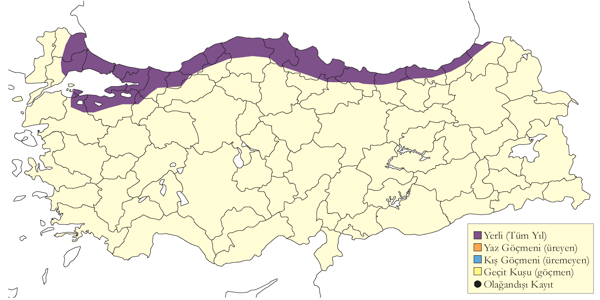
\includegraphics{images/harita_Page_044.png}

\hypertarget{uxfcreme-43}{%
\subsection{\texorpdfstring{\textbf{Üreme}}{Üreme}}\label{uxfcreme-43}}

Bilinen gözlem yoktur.

\textbf{Alttürler ve Sınıflandırma}

Yerli popülasyon çoğu yazarca nominat \emph{colchicus} alttürü olarak
tespit edilmiş\textsuperscript{102,103}, popülasyonu Kuzey Kafkasya'da
bulunan \emph{septentrionalis} alttürü olarak
tanımlamıştır\textsuperscript{28}. Türkiye yerli bir popülasyonunun
varlığını şüpheli görmüştür\textsuperscript{81}. Ancak İstanbul
bölgesinden 1792'lerden itibaren gelen kayıtları ortaya çıkararak
popülasyonun kökeninin yerli kuşlardan oluştuğunu
göstermiştir\textsuperscript{101}.

\bookmarksetup{startatroot}

\hypertarget{kaynakuxe7a}{%
\chapter*{Kaynakça}\label{kaynakuxe7a}}
\addcontentsline{toc}{chapter}{Kaynakça}

\markboth{Kaynakça}{Kaynakça}

\hypertarget{refs}{}
\begin{CSLReferences}{0}{0}
\leavevmode\vadjust pre{\hypertarget{ref-ost1969}{}}%
\CSLLeftMargin{1. }%
\CSLRightInline{OST, O. S. O. T. \emph{Bird report 1966--67}. (OST,
London, 1969).}

\leavevmode\vadjust pre{\hypertarget{ref-ost1972}{}}%
\CSLLeftMargin{2. }%
\CSLRightInline{OST, O. S. O. T. \emph{Bird report 1968--69}. (OST,
London, 1972).}

\leavevmode\vadjust pre{\hypertarget{ref-ost1975}{}}%
\CSLLeftMargin{3. }%
\CSLRightInline{OST, O. S. O. T. \emph{Bird report 1970--73}. (OST,
London, 1975).}

\leavevmode\vadjust pre{\hypertarget{ref-ost1978}{}}%
\CSLLeftMargin{4. }%
\CSLRightInline{OST, O. S. O. T. \emph{Bird report 1974--75}. (OST,
London, 1978).}

\leavevmode\vadjust pre{\hypertarget{ref-beaman1986}{}}%
\CSLLeftMargin{5. }%
\CSLRightInline{Beaman, M. Turkey bird report 1976--81.
\emph{Sandgrouse} \textbf{8}, 1--41 (1986).}

\leavevmode\vadjust pre{\hypertarget{ref-kirwan2003}{}}%
\CSLLeftMargin{6. }%
\CSLRightInline{Kirwan, G. M., Özen, M., Kurt, B. \& Martins, R. P.
Turkey bird report 1997--2001. \emph{Sandgrouse} \textbf{25}, 8--31
(2003).}

\leavevmode\vadjust pre{\hypertarget{ref-kirwan2006apress}{}}%
\CSLLeftMargin{7. }%
\CSLRightInline{Kirwan, G. M., Özen, M. \& Demirci, B. (compilers).
Turkey bird report 2002--06. \emph{Sandgrouse 30}.}

\leavevmode\vadjust pre{\hypertarget{ref-kirwan2014}{}}%
\CSLLeftMargin{8. }%
\CSLRightInline{Kirwan, G. M. \& Özen, E., M. Turkey bird report
2007--2011. \emph{Sandgrouse} \textbf{36}, (2014).}

\leavevmode\vadjust pre{\hypertarget{ref-kirwanmartins1994}{}}%
\CSLLeftMargin{9. }%
\CSLRightInline{Kirwan, G. M. \& Martins, R. P. Turkey bird report
1987--91. \emph{Sandgrouse} \textbf{16}, 76--117 (1994).}

\leavevmode\vadjust pre{\hypertarget{ref-kirwanmartins2000}{}}%
\CSLLeftMargin{10. }%
\CSLRightInline{Kirwan, G. M. \& Martins, R. P. Turkey bird report
1992--1996. \emph{Sandgrouse} \textbf{22}, 13--35 (2000).}

\leavevmode\vadjust pre{\hypertarget{ref-martins1989}{}}%
\CSLLeftMargin{11. }%
\CSLRightInline{Martins, R. P. Turkey bird report 1982--86.
\emph{Sandgrouse} \textbf{11}, 1--41 (1989).}

\leavevmode\vadjust pre{\hypertarget{ref-dogalhayati1993}{}}%
\CSLLeftMargin{12. }%
\CSLRightInline{DHKD, D. H. K. D. \emph{Results of the international
waterfowl census turkey 1993. Bird section report no. 7}. (1993).}

\leavevmode\vadjust pre{\hypertarget{ref-dogalhayati1999}{}}%
\CSLLeftMargin{13. }%
\CSLRightInline{DHKD, D. H. K. D. \emph{Results of the international
waterfowl census turkey 1999. Biodiversity programme report no. 10}.
(1999).}

\leavevmode\vadjust pre{\hypertarget{ref-caglayan2005}{}}%
\CSLLeftMargin{14. }%
\CSLRightInline{Çağlayan, E., Kılıç, D. T., Per, E. \& Gem, E. Türkiye
kış ortası sukuşu sayımları 2005. \emph{Doğa Derneği, Ankara} (2005).}

\leavevmode\vadjust pre{\hypertarget{ref-morozov2004}{}}%
\CSLLeftMargin{15. }%
\CSLRightInline{Morozov, V. V. \& Aarvak, T. Wintering of lesser
white-fronted geese breeding in the polar urals. \emph{Casarca}
\textbf{10}, 156--162 (2004).}

\leavevmode\vadjust pre{\hypertarget{ref-aou2000}{}}%
\CSLLeftMargin{16. }%
\CSLRightInline{(AOU), A. O. U. Forty-second supplement to the american
ornithologists' union check-list of north american birds. \emph{Auk}
\textbf{117}, 847--858 (2000).}

\leavevmode\vadjust pre{\hypertarget{ref-kasparek1988a}{}}%
\CSLLeftMargin{17. }%
\CSLRightInline{Kasparek, M. \emph{Der bafasee. Natur und geschichte in
der türkischen ägäis}. (Kasparek Verlag, 1988).}

\leavevmode\vadjust pre{\hypertarget{ref-kumerloeve1970a}{}}%
\CSLLeftMargin{18. }%
\CSLRightInline{Kumerloeve, H. Zur kenntnis der avifauna kleinasiens und
der europäischen türkei (ergänzungen -- hinweise -- fragestellungen).
\emph{Istanbul Fen. Fak. Mecm. B} \textbf{35}, 85--160 (1970a).}

\leavevmode\vadjust pre{\hypertarget{ref-schrader1891}{}}%
\CSLLeftMargin{19. }%
\CSLRightInline{Schrader, G. Ornithologische beobachtungen auf meinen
sammelreisen i. Kleinasien (aidin und mersina). III. syrien. \emph{Orn.
Jber.} \textbf{2}, 179--197, 215--223 (1891).}

\leavevmode\vadjust pre{\hypertarget{ref-dijksen1988}{}}%
\CSLLeftMargin{20. }%
\CSLRightInline{Dijksen, L. J. \& Kasparek, M. \emph{The birds of
acıgöl}. (Kasparek Verlag, Heidelberg, 1988).}

\leavevmode\vadjust pre{\hypertarget{ref-matheydupraz1920}{}}%
\CSLLeftMargin{21. }%
\CSLRightInline{Mathey-Dupraz, A. Notes ornithologiques de la région du
bosphore. \emph{Orn. Beob.} \textbf{17}, 25--29, 108-110; 18: 25-27,
38--41, 55--58, 101--104, 137--139, 157--158, 183-187; 19: 22-25,
41--43, 58--61, 116--119, 156-159; 20: 9-12, 24--27, 118--120, 135--137
(1920--24).}

\leavevmode\vadjust pre{\hypertarget{ref-handrinos1997}{}}%
\CSLLeftMargin{22. }%
\CSLRightInline{Handrinos, G. \& Akriotis, T. \emph{The birds of
greece}. (Christopher Helm, London, 1997).}

\leavevmode\vadjust pre{\hypertarget{ref-kumerloeve1966d}{}}%
\CSLLeftMargin{23. }%
\CSLRightInline{Kumerloeve, H. Ergänzungen zur avifauna kleinasiens.
\emph{Bonn. Zool. Beitr.} \textbf{17}, 257--259 (1966).}

\leavevmode\vadjust pre{\hypertarget{ref-dijksen1985}{}}%
\CSLLeftMargin{24. }%
\CSLRightInline{Dijksen, L. J. \& Kasparek, M. \emph{The birds of
kızılirmak delta}. (Kasparek Verlag, Heidelberg, 1985).}

\leavevmode\vadjust pre{\hypertarget{ref-makatsch1950}{}}%
\CSLLeftMargin{25. }%
\CSLRightInline{Makatsch, W. \emph{Die vogelwelt macedoniens}. (1950).}

\leavevmode\vadjust pre{\hypertarget{ref-kumerloeve1964a}{}}%
\CSLLeftMargin{26. }%
\CSLRightInline{Kumerloeve, H. Zur sumpf- und wasservogelfauna der
türkei. \emph{J. Orn.} \textbf{105}, 307--325 (1964).}

\leavevmode\vadjust pre{\hypertarget{ref-kasparek1983}{}}%
\CSLLeftMargin{27. }%
\CSLRightInline{Kasparek, M. \& Ven, J. van der. \emph{The birds of
erçek gölü. Birds of turkey 1}. (Kasparek Verlag, 1983).}

\leavevmode\vadjust pre{\hypertarget{ref-kumerloeve1961}{}}%
\CSLLeftMargin{28. }%
\CSLRightInline{Kumerloeve, H. Zur kenntnis der avifauna kleinasiens.
\emph{Bonn. Zool. Beitr.} \textbf{12}, 1--318 (1961).}

\leavevmode\vadjust pre{\hypertarget{ref-kilic1990}{}}%
\CSLLeftMargin{29. }%
\CSLRightInline{Kılıç, A. \& Kasparek, M. The ereğli marshes: Assessment
of their biological importance and recommendations for conservation.
\emph{Unpubl. report to International Council for Bird
Preservation/World Wildlife Fund} (1990).}

\leavevmode\vadjust pre{\hypertarget{ref-selous1900}{}}%
\CSLLeftMargin{30. }%
\CSLRightInline{Selous, F. C. A fortnight's egg-collecting in asia
minor. \emph{Ibis (4)} \textbf{4}, 405--424 (1900).}

\leavevmode\vadjust pre{\hypertarget{ref-article}{}}%
\CSLLeftMargin{31. }%
\CSLRightInline{Vangeluwe, D. \emph{et al.}
\href{https://doi.org/10.1134/S1062359018070178}{Migrations of bewick's
swan (cygnus bewickii): New data on tagging the migration routes,
stopovers, and wintering sites}. \emph{Biology Bulletin} \textbf{45},
1230--1242 (2018).}

\leavevmode\vadjust pre{\hypertarget{ref-boyla1998a}{}}%
\CSLLeftMargin{32. }%
\CSLRightInline{Boyla, K. A. \& Eken, G. Remarkable sightings.
\emph{Turna} \textbf{1}, 35--40 (1998).}

\leavevmode\vadjust pre{\hypertarget{ref-brazil2003}{}}%
\CSLLeftMargin{33. }%
\CSLRightInline{Brazil, M. A. \emph{The whooper swan}. (T. \& A. D.
Poyser, London, 2003).}

\leavevmode\vadjust pre{\hypertarget{ref-adizel1998}{}}%
\CSLLeftMargin{34. }%
\CSLRightInline{Adızel, Ö. Van gölü havzası ornithofaunası üzerine
araştırmalar. (Van 100 Yıl Üniversitesi, 1998).}

\leavevmode\vadjust pre{\hypertarget{ref-dogalhayati1992}{}}%
\CSLLeftMargin{35. }%
\CSLRightInline{DHKD, D. H. K. D. \emph{Results of the international
waterfowl census turkey 1992. Bird section report no. 6}. (1992).}

\leavevmode\vadjust pre{\hypertarget{ref-kasparek1992a}{}}%
\CSLLeftMargin{36. }%
\CSLRightInline{Kasparek, M. \emph{Die vögel der türkei: Eine
übersicht}. (Kasparek Verlag, 1992).}

\leavevmode\vadjust pre{\hypertarget{ref-vaurie1965}{}}%
\CSLLeftMargin{37. }%
\CSLRightInline{Vaurie, C. \emph{The birds of the palearctic fauna.
Non-passeriformes}. (H. F. \& G. Witherby, London, 1965).}

\leavevmode\vadjust pre{\hypertarget{ref-kumerloeve1967a}{}}%
\CSLLeftMargin{38. }%
\CSLRightInline{Kumerloeve, H. Neue beiträge zur kenntnis der avifauna
nordost- und ost-kleinasiens. \emph{Istanbul Üniv. Fen. Fak. Mecm. B}
\textbf{32}, 79--213 (1967a).}

\leavevmode\vadjust pre{\hypertarget{ref-baumgart1995}{}}%
\CSLLeftMargin{39. }%
\CSLRightInline{Baumgart, W., Kasparek, M. \& Stephan, B. \emph{Die
vögel syriens: Eine übersicht}. (Kasparek Verlag, 1995).}

\leavevmode\vadjust pre{\hypertarget{ref-eken1997a}{}}%
\CSLLeftMargin{40. }%
\CSLRightInline{Eken, G. The breeding populations of some species of
waterbirds at gediz delta, western turkey. \emph{Zool. Middle East}
\textbf{14}, 53--68 (1997a).}

\leavevmode\vadjust pre{\hypertarget{ref-tucker1994}{}}%
\CSLLeftMargin{41. }%
\CSLRightInline{Tucker, G. \& Heath, M. F. \emph{Birds in europe: Their
conservation status}. (BirdLife International (Conservation Series No.
3), 1994).}

\leavevmode\vadjust pre{\hypertarget{ref-emirogullari_inprep}{}}%
\CSLLeftMargin{42. }%
\CSLRightInline{Emirogullari, E. F., Sonmez, E., Özesmi, S. \& Özesmi,
U. Status of ruddy shelduck tadorna ferruginea in turkey.}

\leavevmode\vadjust pre{\hypertarget{ref-kasparek1987a}{}}%
\CSLLeftMargin{43. }%
\CSLRightInline{Kasparek, M. \emph{The birds of kulu gölü. Birds of
turkey 5}. (Kasparek Verlag, 1987).}

\leavevmode\vadjust pre{\hypertarget{ref-hustings1994}{}}%
\CSLLeftMargin{44. }%
\CSLRightInline{Hustings, F. \& Dijk, K. van. Bird census in the
kizilirmak delta, turkey, in spring 1992. \emph{WIWO (Report No. 45)}
Zeist (1994).}

\leavevmode\vadjust pre{\hypertarget{ref-ertan1996}{}}%
\CSLLeftMargin{45. }%
\CSLRightInline{Ertan, K. T. The birds of kocaçay delta. \emph{Birds of
Turkey} \textbf{12}, (1996).}

\leavevmode\vadjust pre{\hypertarget{ref-boyla2018}{}}%
\CSLLeftMargin{46. }%
\CSLRightInline{Boyla, K. A., Sinav, L. \& Dizdaroğlu, D. E.
\emph{Türkiye üreyen kuş atlası}. (2018).}

\leavevmode\vadjust pre{\hypertarget{ref-schubert1979}{}}%
\CSLLeftMargin{47. }%
\CSLRightInline{Schubert, W. Bemerkenswerte brutnachweise und
brutzeitfeststellungen in anatolien/türkei. \emph{Vogelwelt}
\textbf{100}, 151--155 (1979).}

\leavevmode\vadjust pre{\hypertarget{ref-kirwan1993a}{}}%
\CSLLeftMargin{48. }%
\CSLRightInline{Kirwan, G. M. The birds of hotamış. \emph{Birds of
Turkey} \textbf{9}, (1993).}

\leavevmode\vadjust pre{\hypertarget{ref-kumerloeve1963a}{}}%
\CSLLeftMargin{49. }%
\CSLRightInline{Kumerloeve, H. L'avifaune du lac d'antioche (amik
gölü-gölbasi) et de ses alentours. \emph{Alauda} \textbf{30}, 110--136,
161--211 (1963).}

\leavevmode\vadjust pre{\hypertarget{ref-grimmett1989}{}}%
\CSLLeftMargin{50. }%
\CSLRightInline{Grimmett, R. F. A. \& Jones, T. A. \emph{Important bird
areas in europe}. (International Council for Bird Preservation,
Cambridge, 1989).}

\leavevmode\vadjust pre{\hypertarget{ref-green1993}{}}%
\CSLLeftMargin{51. }%
\CSLRightInline{Green, A. J. \emph{The status and conservation of the
marbled teal marmaronetta angustirostris}. (IWRB (Spec. Publ. No. 23),
Slimbridge, 1993).}

\leavevmode\vadjust pre{\hypertarget{ref-vielliard1968resultats}{}}%
\CSLLeftMargin{52. }%
\CSLRightInline{Vielliard, J. Résultats ornithologiques d'une mission à
travers la turquie. \emph{Istanbul Fen. Fak. Mecm.} \textbf{33}, 67--170
(1968).}

\leavevmode\vadjust pre{\hypertarget{ref-welch1998b}{}}%
\CSLLeftMargin{53. }%
\CSLRightInline{Welch, G. \& Welch, H. Breeding bird survey of uluabat
gölü ramsar site -- 15 may to 20 june 1998. \emph{Unpubl. report}
(1998b).}

\leavevmode\vadjust pre{\hypertarget{ref-kirwan1997b}{}}%
\CSLLeftMargin{54. }%
\CSLRightInline{Kirwan, G. M. The status of the ferruginous duck
\emph{aythya nyroca} in turkey. \emph{Bird Conserv. Intern.} \textbf{7},
345--356 (1997).}

\leavevmode\vadjust pre{\hypertarget{ref-pforr1982}{}}%
\CSLLeftMargin{55. }%
\CSLRightInline{Pforr, M. \& Limbrunner, A. \emph{The breeding birds of
europe: A photographic handbook}. (Croom Helm, Beckenham, 1982).}

\leavevmode\vadjust pre{\hypertarget{ref-meinertzhagen1935}{}}%
\CSLLeftMargin{56. }%
\CSLRightInline{Meinertzhagen, R. Ornithological results of a trip to
syria and adjacent countries in 1933. \emph{Ibis (13)} \textbf{5},
110--151 (1935).}

\leavevmode\vadjust pre{\hypertarget{ref-magninyarar1997}{}}%
\CSLLeftMargin{57. }%
\CSLRightInline{Magnin, G. \& Yarar, M. \emph{Important bird areas in
turkey}. (Doğal Hayatı Koruma Derneği, Istanbul, 1997).}

\leavevmode\vadjust pre{\hypertarget{ref-alleon1880}{}}%
\CSLLeftMargin{58. }%
\CSLRightInline{Alléon, C. A. Catalogue des oiseaux observés aux
environs de constantinople. \emph{Bull. Zool. Soc. France} \textbf{5},
80--116 (1880).}

\leavevmode\vadjust pre{\hypertarget{ref-kirwan1997a}{}}%
\CSLLeftMargin{59. }%
\CSLRightInline{Kirwan, G. M. A list of bird specimens held in the
robert's college, bebek (istanbul, turkey) collection, with some
comments on mathey-dupraz (1920--24). \emph{Sandgrouse} \textbf{19},
30--38 (1997).}

\leavevmode\vadjust pre{\hypertarget{ref-ogilvie1954}{}}%
\CSLLeftMargin{60. }%
\CSLRightInline{Ogilvie, I. H. Bird notes from northern asia minor
1946--1948. \emph{Ibis} \textbf{96}, 81--90 (1954).}

\leavevmode\vadjust pre{\hypertarget{ref-kasparek1990a}{}}%
\CSLLeftMargin{61. }%
\CSLRightInline{Kasparek, M. Zum vorkommen einiger in der türkei
seltener vogelarten. \emph{Bonn. Zool. Beitr.} \textbf{41}, 181--202
(1990).}

\leavevmode\vadjust pre{\hypertarget{ref-welch1998a}{}}%
\CSLLeftMargin{62. }%
\CSLRightInline{Welch, G. \& Welch, H. Results of a survey of wintering
waterbirds along the turkish black sea coast -- 16 january to 7 february
1997. \emph{Turna} \textbf{1}, 16--23 (1998a).}

\leavevmode\vadjust pre{\hypertarget{ref-vanderven1980birds}{}}%
\CSLLeftMargin{63. }%
\CSLRightInline{Ven, G. van der, J. A. Birds in eastern turkey II.
(1980).}

\leavevmode\vadjust pre{\hypertarget{ref-yarar1995aktas}{}}%
\CSLLeftMargin{64. }%
\CSLRightInline{Yarar, M. Aktaş gölü: A new pelican breeding site on the
turkish--georgian border. \emph{Orn. Soc. Middle East Bull.}
\textbf{35}, 46--48 (1995).}

\leavevmode\vadjust pre{\hypertarget{ref-kruper1875}{}}%
\CSLLeftMargin{65. }%
\CSLRightInline{Krüper, T. Beitrag zur ornithologie kleinasiens.
\emph{J. Orn.} \textbf{23}, 258--285 (1875).}

\leavevmode\vadjust pre{\hypertarget{ref-balmer2004b}{}}%
\CSLLeftMargin{66. }%
\CSLRightInline{Balmer, D. \& Betton, K. Around the region.
\emph{Sandgrouse} \textbf{26}, 160--168 (2004b).}

\leavevmode\vadjust pre{\hypertarget{ref-demirci2002}{}}%
\CSLLeftMargin{67. }%
\CSLRightInline{Demirci, B. Toygardan kayıtlar (ocak--mart 2002).
\emph{Kuşçu Bulteni} \textbf{11}, 6--7 (2002).}

\leavevmode\vadjust pre{\hypertarget{ref-scott1982}{}}%
\CSLLeftMargin{68. }%
\CSLRightInline{Scott, D. A. \& Carp, E. A midwinter survey of wetlands
in mesopotamia, iraq: 1979. \emph{Sandgrouse} \textbf{4}, 60--76
(1982).}

\leavevmode\vadjust pre{\hypertarget{ref-adamian1999}{}}%
\CSLLeftMargin{69. }%
\CSLRightInline{Adamian, M. S. \& Klem, D. \emph{Handbook of the birds
of armenia}. (American University of Armenia, 1999).}

\leavevmode\vadjust pre{\hypertarget{ref-eken1997d}{}}%
\CSLLeftMargin{70. }%
\CSLRightInline{Eken, G. The wintering populations of some waterbird
species on the mediterranean coastline of turkey. 61--69 (1997d).}

\leavevmode\vadjust pre{\hypertarget{ref-kumerloeve1966-67}{}}%
\CSLLeftMargin{71. }%
\CSLRightInline{Kumerloeve, H. Migration et hivernage sur le lac
d'antioche (amik gölü, hatay, turquie); coup l'oeil sur son avifaune
nidificatrice actuelle. \emph{Alauda} \textbf{34}, 299-308; 35: 1-19
(1966-67).}

\leavevmode\vadjust pre{\hypertarget{ref-kirwan1994b}{}}%
\CSLLeftMargin{72. }%
\CSLRightInline{Kirwan, G. M. The breeding status and distribution of
the white-headed duck (\emph{oxyura leucocephala}) on the central
plateau, turkey. \emph{Sandgrouse} \textbf{16}, 66--75 (1994).}

\leavevmode\vadjust pre{\hypertarget{ref-richardson2003}{}}%
\CSLLeftMargin{73. }%
\CSLRightInline{Richardson, I. M. A long-term bird survey of kulu gölü,
turkey (2001--2002). \emph{Sandgrouse} \textbf{25}, 110--121 (2003).}

\leavevmode\vadjust pre{\hypertarget{ref-green1992}{}}%
\CSLLeftMargin{74. }%
\CSLRightInline{Green, A. J. \& Anstey, S. The status of the
white-headed duck \emph{oxyura leucocephala}. \emph{Bird Conserv.
Intern.} \textbf{2}, 185--200 (1992).}

\leavevmode\vadjust pre{\hypertarget{ref-anstey1989}{}}%
\CSLLeftMargin{75. }%
\CSLRightInline{Anstey, S. \emph{The status and conservation of the
white-headed duck ({Oxyura leucocephala})}. (IWRB (Spec. Publ. No. 10),
1989).}

\leavevmode\vadjust pre{\hypertarget{ref-rigler1852}{}}%
\CSLLeftMargin{76. }%
\CSLRightInline{Rigler, L. \emph{Die türkei und deren bewohner in ihren
naturhistorischen, physiologischen und pathologischen verhältnissen vom
standpunkte constantinopel's}. (Wien, 1852).}

\leavevmode\vadjust pre{\hypertarget{ref-tchihatchef1864}{}}%
\CSLLeftMargin{77. }%
\CSLRightInline{Tchihatchef, P. de. \emph{Le bosphore et
constantinople}. (Paris, 1864).}

\leavevmode\vadjust pre{\hypertarget{ref-reiser1904}{}}%
\CSLLeftMargin{78. }%
\CSLRightInline{Reiser, O. Zur kenntnis der vogelwelt von
konstantinopel. \emph{Orn. Jahrb.} \textbf{15}, 153--156 (1904).}

\leavevmode\vadjust pre{\hypertarget{ref-elwes1870}{}}%
\CSLLeftMargin{79. }%
\CSLRightInline{Elwes, H. J. \& Buckley, T. E. A list of the birds of
turkey. \emph{Ibis (II)} \textbf{6}, 59--77, 327--341 (1870).}

\leavevmode\vadjust pre{\hypertarget{ref-hagemeijer1997}{}}%
\CSLLeftMargin{80. }%
\CSLRightInline{Hagemeijer, W. J. M. \& Blair, M. J. \emph{The EBCC
atlas of european breeding birds}. (T. \& A. D. Poyser, London, 1997).}

\leavevmode\vadjust pre{\hypertarget{ref-madge2002}{}}%
\CSLLeftMargin{81. }%
\CSLRightInline{Madge, S. \& McGowan, P. \emph{Pheasants, partridges and
grouse}. (Christopher Helm, London, 2002).}

\leavevmode\vadjust pre{\hypertarget{ref-baskaya2003}{}}%
\CSLLeftMargin{82. }%
\CSLRightInline{Başkaya, S. Distribution and principal threats to
caucasian black grouse ({Tetrao mlokosiewiczi}) in the eastern karadeniz
mountains in turkey. \emph{Wildl. Biol.} \textbf{9}, 377--383 (2003).}

\leavevmode\vadjust pre{\hypertarget{ref-atkinson1995}{}}%
\CSLLeftMargin{83. }%
\CSLRightInline{Atkinson, P. W., Humpage, E. A., Jowitt, A. J. D.,
Oğurlu, I. \& Rowcliffe, J. M. The distribution and status of caucasian
black grouse in north-eastern turkey. \emph{Proc. Intern. Symp. Grouse}
\textbf{6}, 131--133 (1995).}

\leavevmode\vadjust pre{\hypertarget{ref-isfendiyaroglu2007}{}}%
\CSLLeftMargin{84. }%
\CSLRightInline{Isfendiyaroğlu, S., Welch, G. \& Atad, M. The caucasian
black grouse \emph{(tetrao mlokosiewiczi)} in turkey: Recent survey
results and conservation recommendations. \emph{Wildl. Biol. Suppl.}
\textbf{1}, 13--20 (2007).}

\leavevmode\vadjust pre{\hypertarget{ref-gottschalk2007}{}}%
\CSLLeftMargin{85. }%
\CSLRightInline{Gottschalk, T. K., Ekschmitt, K., Isfendiyaroğlu, S.,
Gem, E. \& Wolters, W. Assessing the potential distribution of the
caucasian black grouse tetrao mlokosiewiczi in turkey through spatial
modelling. \emph{J. Orn.} \textbf{148}, 427--434 (2007).}

\leavevmode\vadjust pre{\hypertarget{ref-templelang1991}{}}%
\CSLLeftMargin{86. }%
\CSLRightInline{Temple-Lang, J. \& Cocker, M. A nest of caucasian black
grouse \emph{tetrao mlokosiewiczi} in turkey. \emph{Sandgrouse}
\textbf{13}, 102--103 (1991).}

\leavevmode\vadjust pre{\hypertarget{ref-gokhelashvili2003}{}}%
\CSLLeftMargin{87. }%
\CSLRightInline{Gokhelashvili, R., Reese, K. P. \& Gavashelishvili, L.
How much do we know about the caucasian black grouse tetrao
mlokosiewiczi? \emph{Sandgrouse} \textbf{25}, 32--40 (2003).}

\leavevmode\vadjust pre{\hypertarget{ref-danford1877}{}}%
\CSLLeftMargin{88. }%
\CSLRightInline{Danford, C. G. A contribution to the ornithology of asia
minor. \emph{Ibis (IV)} \textbf{1}, 261--274 (1877-78).}

\leavevmode\vadjust pre{\hypertarget{ref-sutton1972}{}}%
\CSLLeftMargin{89. }%
\CSLRightInline{Sutton, R. W. W. \& Gray, J. R. Summer birds of karanfil
dağ. \emph{Orn. Soc. Turkey Bird Rep.} \textbf{1968--69}, 186--205
(1972).}

\leavevmode\vadjust pre{\hypertarget{ref-ramsay1914}{}}%
\CSLLeftMargin{90. }%
\CSLRightInline{Ramsay, L. N. G. Observations on the bird-life of the
anatolian plateau during the summer of 1907. \emph{Ibis} \textbf{10
(2)}, 365--387 (1914).}

\leavevmode\vadjust pre{\hypertarget{ref-mcneile1950}{}}%
\CSLLeftMargin{91. }%
\CSLRightInline{McNeile, J. S. Personal diaries. (1950, 1951, 1954,
1967, 1968, 1970, 1972, 1973).}

\leavevmode\vadjust pre{\hypertarget{ref-rokitansky1971}{}}%
\CSLLeftMargin{92. }%
\CSLRightInline{Rokitansky, G. \& Schifter, H. Ornithologische
ergebnisse zweier sammelreisen in die türkei. \emph{Ann. Naturhist. Mus.
Wien} \textbf{75}, 495--538 (1971).}

\leavevmode\vadjust pre{\hypertarget{ref-baris1984}{}}%
\CSLLeftMargin{93. }%
\CSLRightInline{Barış, S., Akçakaya, R. \& Bilgin, C. \emph{The birds of
kızılcahamam}. vol. 3 (Kasparek Verlag, 1984).}

\leavevmode\vadjust pre{\hypertarget{ref-zeydanli2005gap}{}}%
\CSLLeftMargin{94. }%
\CSLRightInline{Zeydanlı, U. Z., Welch, H. J., Welch, G. R., Altıntaş,
M. \& Domaç, A. GAP analysis and priority conservation area selection
for mediterranean turkey: Preliminary technical report. (2005).}

\leavevmode\vadjust pre{\hypertarget{ref-welch2004gap}{}}%
\CSLLeftMargin{95. }%
\CSLRightInline{\emph{GAP biodiversity research project 2001--2003 --
final report}. (Doğal Hayatı Koruma Derneği, Istanbul, 2004).}

\leavevmode\vadjust pre{\hypertarget{ref-berk1988}{}}%
\CSLLeftMargin{96. }%
\CSLRightInline{Berk, V. van den. The black francolin in turkey.
\emph{Sandgrouse} \textbf{10}, 51--57 (1988).}

\leavevmode\vadjust pre{\hypertarget{ref-kumerloeve1963c}{}}%
\CSLLeftMargin{97. }%
\CSLRightInline{Kumerloeve, H. Zur brutverbreitung des frankolins,
\emph{francolinus francolinus} (l.) im vorderen orient. \emph{Vogelwelt}
\textbf{84}, 129--137 (1963).}

\leavevmode\vadjust pre{\hypertarget{ref-karakas2002}{}}%
\CSLLeftMargin{98. }%
\CSLRightInline{Karakaş, R. \& Kılıç, A. Birds of göksu dam (diyarbakır)
and new records in south-east turkey. \emph{Sandgrouse} \textbf{24},
38--43 (2002).}

\leavevmode\vadjust pre{\hypertarget{ref-albrecht1986}{}}%
\CSLLeftMargin{99. }%
\CSLRightInline{Albrecht, J. S. M. Notes on the birds of eregli, black
sea coastlands, turkey 1976--1978. \emph{Sandgrouse} \textbf{8}, 74--92
(1986).}

\leavevmode\vadjust pre{\hypertarget{ref-balmer2004a}{}}%
\CSLLeftMargin{100. }%
\CSLRightInline{Balmer, D. \& Betton, K. Around the region.
\emph{Sandgrouse} \textbf{26}, 76--80 (2004a).}

\leavevmode\vadjust pre{\hypertarget{ref-kasparek1988c}{}}%
\CSLLeftMargin{101. }%
\CSLRightInline{Kasparek, M. Zum ursprünglichen vorkommen und zur
wiedereinbürgerung des fasans, \emph{(phasianus colchicus)}, in der
türkei. \emph{Verh. Orn. Ges. Bayern} \textbf{24}, 725--735 (1988).}

\leavevmode\vadjust pre{\hypertarget{ref-dementev1967}{}}%
\CSLLeftMargin{102. }%
\CSLRightInline{Dement'ev, G. P. \& Gladkov, N. A. \emph{Birds of the
soviet union. Vol. 4}. (Israel Program for Scientific Translations,
Jerusalem, 1967).}

\leavevmode\vadjust pre{\hypertarget{ref-roselaar1995}{}}%
\CSLLeftMargin{103. }%
\CSLRightInline{Roselaar, C. S. \emph{Songbirds of turkey: An atlas of
biodiversity in turkish passerine birds}. (Pica Press, Robertsbridge \&
GMB, Haarlem, 1995).}

\end{CSLReferences}



\end{document}
